% A LaTeX template for MSc Thesis submissions to 
% Politecnico di Milano (PoliMi) - School of Industrial and Information Engineering
%
% S. Bonetti, A. Gruttadauria, G. Mescolini, A. Zingaro
% e-mail: template-tesi-ingind@polimi.it
%
% Last Revision: October 2021
%
% Copyright 2021 Politecnico di Milano, Italy. NC-BY

\documentclass{config/polimiThesis}

%------------------------------------------------------------------------------
%	REQUIRED PACKAGES AND  CONFIGURATIONS
%------------------------------------------------------------------------------

% CONFIGURATIONS
\usepackage{parskip}       % For paragraph layout
\usepackage{setspace}      % For using single or double spacing
\usepackage{emptypage}     % To insert empty pages
\usepackage{multicol}      % To write in multiple columns (executive summary)
\setlength\columnsep{15pt} % Column separation in executive summary
\setlength\parindent{0pt}  % Indentation
\raggedbottom  

% PACKAGES FOR TITLES
\usepackage{titlesec}
% \titlespacing{\section}{left spacing}{before spacing}{after spacing}
\titlespacing{\section}{0pt}{3.3ex}{2ex}
\titlespacing{\subsection}{0pt}{3.3ex}{1.65ex}
\titlespacing{\subsubsection}{0pt}{3.3ex}{1ex}
\usepackage{color}
\usepackage{multirow}

% PACKAGES FOR LANGUAGE AND FONT
\usepackage[english]{babel} % The document is in English  
\usepackage[utf8]{inputenc} % UTF8 encoding
\usepackage[T1]{fontenc}    % Font encoding
\usepackage[11pt]{moresize} % Big fonts

% PACKAGES FOR IMAGES
\usepackage{graphicx}
\usepackage{transparent} % Enables transparent images
\usepackage{eso-pic}     % For the background picture on the title page
\usepackage{subfig}      % Numbered and caption subfigures using \subfloat.
\usepackage{float}

\usepackage{tikz}
\usetikzlibrary{
    patterns,
    overlay-beamer-styles,
    datavisualization,
    datavisualization.formats.functions,
    fit,
    trees,
    backgrounds,
    mindmap,
    positioning,
    shapes.geometric,
    arrows
}

\usepackage{pgfplots}  
\usepgfplotslibrary{
    groupplots,
    units
}

\usepackage{pgf-pie}
\usepackage{csvsimple}
\usepackage{pdfpages}

\usepackage{enumitem}
\setitemize{itemsep=-5pt}

\usepackage{relsize}
\usepackage{makecell}

\graphicspath{{./images/}} 

\usepackage{caption}        
\usepackage{amsthm}
\usepackage{thmtools}
\usepackage{xcolor}                 
\usepackage{float}

% STANDARD MATH PACKAGES
\usepackage{amsmath}
\usepackage{amsthm}
\usepackage{amssymb}
\usepackage{amsfonts}
\usepackage{bm}
\usepackage[overload]{empheq} % For braced-style systems of equations.
\usepackage{fix-cm}           % To override original LaTeX restrictions on sizes

% PACKAGES FOR TABLES
\usepackage{tabularx}
\usepackage{longtable} % Tables that can span several pages
\usepackage{colortbl}

% PACKAGES FOR ALGORITHMS (PSEUDO-CODE)
\usepackage{algorithm}
\usepackage{algorithmic}

\usepackage{titlesec}
\setcounter{tocdepth}{4}
\setcounter{secnumdepth}{4}

% PACKAGES FOR REFERENCES & BIBLIOGRAPHY
\usepackage{hyperref}
\hypersetup{
    colorlinks=false, % true
    linkcolor=blue!80!black,
    filecolor=magenta,      
    urlcolor=cyan!80!black,
    citecolor=red!70!black,
    pdftitle={THESIS},
    pdfpagemode=FullPage,
}

\usepackage{cleveref}
\usepackage[square, numbers, sort&compress]{natbib} % Square brackets, citing references with numbers, citations sorted by appearance in the text and compressed
\bibliographystyle{abbrvnat}                        % You may use a different style adapted to your field

% OTHER PACKAGES
\usepackage{pdfpages} % To include a pdf file
\usepackage{afterpage}
\usepackage{fancyhdr} % For the headers
\fancyhf{}

\usepackage{comment}
\usepackage{listings}
\colorlet{numb}{magenta!60!black}

\lstdefinestyle{customPy}{
  belowcaptionskip=1\baselineskip,
  breaklines=true,
  numbers=left,      
  numbersep=6pt, 
  xleftmargin=\parindent,
  language=Python,
  basicstyle=\fontsize{11}{11}\ttfamily,
  showstringspaces=false,
  keywordstyle=\bfseries\color{purple},
  commentstyle=\itshape\color{violet},
  identifierstyle=\color{blue},
  stringstyle=\color{orange},
}

\lstdefinestyle{customTXT}{
    % basicstyle=\small\ttfamily,
    basicstyle=\ttfamily\small,
    commentstyle=\itshape\color{violet}, % style of comment
    stringstyle=\color{blue}, % style of strings
    numbers=left,
    numberstyle=\scriptsize,
    % basicstyle=\ttfamily\footnotesize,  % Style of the font that is used for the code
    % backgroundcolor=\color{gray!10},    % Background color
    % keywordstyle=\color{red!75!black},  % Keyword style
    % stringstyle=\color{magenta!40!black}, % String style
    % commentstyle=\color{green!30!black}, % Comment style
    stepnumber=1,
    numbersep=8pt,
    showstringspaces=false,
    breaklines=true,
    frame=lines,
    backgroundcolor=\color{gray!10}, %only if you like
    string=[s]{"}{"},
    comment=[l]{ !},
    morecomment=[l]{:"},
    literate=
        *{0}{{{\color{black}0}}}{1}
         {1}{{{\color{black}1}}}{1}
         {2}{{{\color{black}2}}}{1}
         {3}{{{\color{black}3}}}{1}
         {4}{{{\color{black}4}}}{1}
         {5}{{{\color{black}5}}}{1}
         {6}{{{\color{black}6}}}{1}
         {7}{{{\color{black}7}}}{1}
         {8}{{{\color{black}8}}}{1}
         {9}{{{\color{black}9}}}{1}
}

\lstdefinelanguage{json}{
    basicstyle=\ttfamily\small,
    commentstyle=\itshape\color{violet},
    stringstyle=\color{blue}, % style of strings
    numbers=left,
    numberstyle=\scriptsize,
    % basicstyle=\ttfamily\footnotesize,  % Style of the font that is used for the code
    % backgroundcolor=\color{gray!10},    % Background color
    % keywordstyle=\color{red!75!black},  % Keyword style
    % stringstyle=\color{magenta!40!black}, % String style
    % commentstyle=\color{green!30!black}, % Comment style
    stepnumber=1,
    numbersep=8pt,
    showstringspaces=false,
    breaklines=true,
    frame=lines,
    backgroundcolor=\color{gray!10}, %only if you like
    string=[s]{"}{"},
    comment=[l]{ //},
    morecomment=[l]{:"},
    literate=
        *{0}{{{\color{black}0}}}{1}
         {1}{{{\color{black}1}}}{1}
         {2}{{{\color{black}2}}}{1}
         {3}{{{\color{black}3}}}{1}
         {4}{{{\color{black}4}}}{1}
         {5}{{{\color{black}5}}}{1}
         {6}{{{\color{black}6}}}{1}
         {7}{{{\color{black}7}}}{1}
         {8}{{{\color{black}8}}}{1}
         {9}{{{\color{black}9}}}{1}
}

% Input of configuration file. Do not change config.tex file unless you really know what you are doing. 
% Set the geometric layout of the document
\usepackage{geometry}
\geometry{
  top=3cm,
  left = 2.0cm,
  right = 2.0cm,
  bottom=2cm,
  headheight= 2cm,
  headsep= 0cm,
}
\raggedbottom 

% Create color bluePoli (-> manuale grafica coordinata:  https://www.polimi.it/fileadmin/user_upload/il_Politecnico/grafica-coordinata/2015_05_11_46xy_manuale_grafica_coordinata.pdf)
\definecolor{bluePoli}{cmyk}{0.4,0.1,0,0.4}

% Custom theorem environments
\declaretheoremstyle[
  headfont=\color{bluePoli}\normalfont\bfseries,
  bodyfont=\color{black}\normalfont\itshape,
]{colored}

\captionsetup[figure]{labelfont={color=bluePoli}} % Set colour of the captions
\captionsetup[table]{labelfont={color=bluePoli}} % Set colour of the captions
\captionsetup[algorithm]{labelfont={color=bluePoli}} % Set colour of the captions

\theoremstyle{colored}
\newtheorem{theorem}{Theorem}[section]
\newtheorem{proposition}{Proposition}[section]

% Enhances the features of the standard "table" and "tabular" environments.
\newcommand\T{\rule{0pt}{2.6ex}}
\newcommand\B{\rule[-1.2ex]{0pt}{0pt}}

% Algorithm description
\newcounter{algsubstate}
\renewcommand{\thealgsubstate}{\alph{algsubstate}}
\newenvironment{algsubstates}{
    \setcounter{algsubstate}{0}%
    \renewcommand{\STATE}{%
    \stepcounter{algsubstate}%
    \Statex {\small\thealgsubstate:}\space}
    }{}
    
% Custom theorem environment
\newcolumntype{L}[1]{>{\raggedright\let\newline\\\arraybackslash\hspace{0pt}}m{#1}}
\newcolumntype{C}[1]{>{\centering\let\newline\\\arraybackslash\hspace{0pt}}m{#1}}
\newcolumntype{R}[1]{>{\raggedleft\let\newline\\\arraybackslash\hspace{0pt}}m{#1}}

% Custom itemize environment
\setlist[itemize,1]{label=$\bullet$}
\setlist[itemize,2]{label=$\circ$}
\setlist[itemize,3]{label=$-$}
\setlist{nosep}

% Set separation of columns 
\setlength{\columnsep}{30pt}

% Create command for background pic
\newcommand\BackgroundPic{% Adding background picture
	\put(230,358){
		\parbox[b][\paperheight]{\paperwidth}{%
			\vfill
			\centering
			\transparent{0.4}
			
\includegraphics[width=0.5\paperwidth]{raggiera_polimi.eps}%
			\vfill
}}}

% Set indentation
\setlength\parindent{0pt}

% Custom title commands
\titleformat{\section}
{\color{bluePoli}\normalfont\Large\bfseries}
{\color{bluePoli}\thesection.}{1em}{}
\titlespacing*{\section}
{0pt}{2ex}{1ex}

\titleformat{\subsection}
{\color{bluePoli}\normalfont\large\bfseries}
{\color{bluePoli}\thesubsection.}{1em}{}
\titlespacing*{\subsection}
{0pt}{2ex}{1ex}

% Custom headers and footers
\pagestyle{fancy}
\fancyhf{}
      
\fancyfoot{}
\fancyfoot[C]{\thepage} % page
\renewcommand{\headrulewidth}{0mm} % headrule width
\renewcommand{\footrulewidth}{0mm} % footrule width

\makeatletter
\patchcmd{\headrule}{\hrule}{\color{black}\hrule}{}{} % headrule
\patchcmd{\footrule}{\hrule}{\color{black}\hrule}{}{} % footrule
\makeatother

% -> Create the header
\chead[C]{
\centering
\begin{tcolorbox}[arc=0pt, boxrule=0pt, colback=bluePoli!60, width=\textwidth, colupper=white]
    \textbf{Executive summary} \hfill \textbf{\author}  
\end{tcolorbox}
}

%----------------------------------------------------------------------------
%	NEW COMMANDS DEFINED
%----------------------------------------------------------------------------

% EXAMPLES OF NEW COMMANDS
\newcommand{\bea}{\begin{eqnarray}} % Shortcut for equation arrays
\newcommand{\eea}{\end{eqnarray}}
\newcommand{\e}[1]{\times 10^{#1}}  % Powers of 10 notation

\newenvironment{dedication}
{%\clearpage           % we want a new page          %% I commented this
\thispagestyle{empty}% no header and footer
\vspace*{\stretch{1}}% some space at the top
\itshape             % the text is in italics
\raggedleft          % flush to the right margin
}
{\par % end the paragraph
\vspace{\stretch{3}} % space at bottom is three times that at the top
\clearpage           % finish off the page
}

%----------------------------------------------------------------------------
%	ADD YOUR PACKAGES (be careful of package interaction)
%----------------------------------------------------------------------------

%----------------------------------------------------------------------------
%	ADD YOUR DEFINITIONS AND COMMANDS (be careful of existing commands)
%----------------------------------------------------------------------------

%----------------------------------------------------------------------------
%	BEGIN OF YOUR DOCUMENT
%----------------------------------------------------------------------------

\begin{document}

\fancypagestyle{plain}{%
\fancyhf{} % Clear all header and footer fields
\fancyhead[RO,RE]{\thepage} %RO=right odd, RE=right even
\renewcommand{\headrulewidth}{0pt}
\renewcommand{\footrulewidth}{0pt}}

%----------------------------------------------------------------------------
%	TITLE PAGE
%----------------------------------------------------------------------------

\pagestyle{empty} % No page numbers
\frontmatter % Use roman page numbering style (i, ii, iii, iv...) for the preamble pages

\puttitle{
	title = Data Driven Approach \\ to Turbomachinery Blade Design, % Title of the thesis
	name = Antonio Pucciarelli, % Author Name and Surname
	course = Aeronautical Engineering, % Study Programme (in Italian)
	ID = 974675,  % Student ID number (numero di matricola)
	advisor = Prof. Sergio Lavagnoli, % Supervisor name
	promoter = Prof. Paolo Gaetani,
    % coadvisor = {Prof. Paolo Gaetani}, % Co-Supervisor name, remove this line if there is none
	academicyear = {2022-2023},  % Academic Year
} % These info will be put into your Title page 



%----------------------------------------------------------------------------
%	PREAMBLE PAGES: ABSTRACT (inglese e italiano), EXECUTIVE SUMMARY
%----------------------------------------------------------------------------
\newpage
% \AddToShipoutPicture*{\BackgroundPic}
\blankpage
\setcounter{page}{1} % Set page counter to 1

% ABSTRACT IN ENGLISH
% \chapter*{Abstract} 
% % Here goes the Abstract in English of your thesis followed by a list of keywords.
% % The Abstract is a concise summary of the content of the thesis (single page of text)
% % and a guide to the most important contributions included in your thesis.
% % The Abstract is the very last thing you write.
% % It should be a self-contained text and should be clear to someone who hasn't (yet) read the whole manuscript.
% % The Abstract should contain the answers to the main scientific questions that have been addressed in your thesis.
% % It needs to summarize the adopted motivations and the adopted methodological approach as well as the findings of your work and their relevance and impact.
% % The Abstract is the part appearing in the record of your thesis inside POLITesi,
% % the Digital Archive of PhD and Master Theses (Laurea Magistrale) of Politecnico di Milano.
% % The Abstract will be followed by a list of four to six keywords.
% % Keywords are a tool to help indexers and search engines to find relevant documents.
% % To be relevant and effective, keywords must be chosen carefully.
% % They should represent the content of your work and be specific to your field or sub-field.
% % Keywords may be a single word or two to four words. 
% In the field of turbomachinery design, the current design models are often slow and repetitive. These models rely heavily on computers and frequently overlook any existing knowledge about the design space. This work introduces an innovative methodology in the domain of turbomachinery design, seamlessly integrating machine learning techniques into the blade design process.

% The importance of this thesis lies in its ability to eliminate the requirement for CFD simulations in the design process. Moreover, it gives designers a clear understanding of the loading limit of a blade and a deep understanding of the correlations between the loading distribution and the blade geometry. It also sheds light on the physical limitations a designer might come across during the design process.

% % The process begins with the generation of an extensive database, achieved through an in-depth analysis of the main design objectives. This forms the basis for applying artificial intelligence in the field of turbomachinery blade design. The thesis adopts a modal reduction technique that effectively refines and narrows the extensive design space, providing a better understanding of the correlation between the loading distribution and the blade geometry.

% Highlighting the significant influence of this study, the thesis not only presents a fresh design approach but also offers in-depth understanding of the crucial steps that support its implementation. Covering the entire process from creating data to utilizing artificial intelligence in turbomachinery design, this research sets the groundwork for more effective design strategies.

% To sum up, this thesis introduces a new approach to designing turbomachinery blades through the integration of machine learning methods. By creating a fast and independent design process and providing a clear explanation of how data is collected and analyzed, this research brings improved efficiency and accuracy to the world of turbomachinery design.
% \\
% \\
% % \textbf{Keywords:} \textit{Turbomachinery, data generation, optimization, data analysis, artificial intelligence, principal component analysis} % Keywords
% \textbf{Keywords:} \textit{Turbomachinery, data analysis, artificial intelligence, modal reduction}

% % ABSTRACT IN ITALIAN
% \chapter*{Abstract in lingua italiana}
% Nel campo della progettazione di turbomacchine, i modelli di progettazione attuali sono spesso lenti e ripetitivi. Questi modelli si basano pesantemente sui computer e spesso trascurano qualsiasi conoscenza esistente dello spazio di progettazione. Questo lavoro introduce una metodologia innovativa nel campo della progettazione di turbomacchine, integrando delle tecniche di intelligenza artificiale per la progettazione di palette di turbina.

% L'importanza di questa tesi risiede nella sua capacità di eliminare la necessità di simulazioni CFD nel processo di progettazione di palette per turbomacchine. Inoltre, fornisce ai progettisti una chiara visione del limite di carico di una pala e una buona descirzione delle correlazioni tra la distribuzione del carico e la geometria della pala. Inoltre, getta luce sulle limitazioni fisiche che un progettista potrebbe incontrare durante il processo di progettazione.

% % Il processo inizia con la generazione di un ampio database, ottenuto attraverso un'analisi approfondita degli obiettivi principali di progettazione. Questo costituisce la base per l'applicazione dell'intelligenza artificiale nel campo della progettazione di pale per turbomacchine. La tesi adotta una tecnica di riduzione modale che affina ed restringe efficacemente l'ampio spazio di progettazione, fornendo una migliore comprensione della correlazione tra la distribuzione del carico e la geometria.

% Evidenziando l'influenza significativa di questo studio, la tesi non solo presenta un approccio di progettazione innovativo, ma offre anche una comprensione approfondita dei passaggi cruciali che ne sostengono l'attuazione. Coprendo l'intero processo dalla creazione dei dati all'utilizzo dell'intelligenza artificiale nella progettazione di turbomacchine, questa ricerca getta le basi per strategie di metodi di progettazione più efficaci.

% In sintesi, questa tesi introduce un nuovo approccio alla progettazione delle pale per turbomacchine. Creando un processo di progettazione rapido e indipendente e fornendo una spiegazione chiara di come vengono raccolti e analizzati i dati, questa ricerca introduce l'integrazione dell'intelligenza artificiale nella progettazione di turbomacchine.
% \\
% \\
% % \textbf{Parole chiave:} \textit{Turbomacchine, generazione di dati, ottimizzazione, analisi di dati, intelligenza artificiale, riduzione modale} % Keywords (italian)
% \textbf{Parole chiave:} \textit{Turbomacchine, analisi di dati, intelligenza artificiale, riduzione modale} % Keywords (italian)

%----------------------------------------------------------------------------
%	LIST OF CONTENTS/FIGURES/TABLES/SYMBOLS
%----------------------------------------------------------------------------

% \cleardoublepage
% \thispagestyle{empty}
% \epigraph{Discipline, doing what you hate to do but do it like you love it.}{\textit{Mike Tyson}}
% \cleardoublepage
% \cleardoublepage
% \begin{dedication}

%     Ad Alessandro, \\ Lucia e \\ Valerio, \\ la mia Famiglia. 
  
%     \vspace{\baselineskip}
    
%     \usefont{T1}{LobsterTwo-LF}{bx}{it}
%     Antonio

% \end{dedication}

% TABLE OF CONTENTS
% \thispagestyle{empty}
% \tableofcontents % Table of contents 
% \thispagestyle{empty}
% \cleardoublepage

% LIST OF FIGURES
% \listoffigures

% LIST OF TABLES
% \listoftables

% LIST OF SYMBOLS
% Write out the List of Symbols in this page
% \chapter*{List of Symbols} % You have to include a chapter for your list of symbols (
% \begin{table}[H]
    % \centering
    % \begin{tabular}{lll}
        % \textbf{Variable} & \textbf{Description} & \textbf{SI unit} \\\hline\\[-9px]
        % $\bm{u}$ & solid displacement & m \\[2px]
        % $\bm{u}_f$ & fluid displacement & m \\[2px]
    % \end{tabular}
% \end{table}

% \chapter*{List of Abbreviations}

% \begin{longtable}{p{2.5cm}p{8cm}}
%     % \toprule
%     \hline
%     Abbreviation & Definition \\
%     % \midrule\endhead % Add abbreviations alphabetically here:
%     \hline
%     \texttt{SINL} & Inlet slope \\
%     \texttt{SOUT} & Outlet slope \\ 
%     \texttt{KUTTA} & Kutta condition \\ 
%     \texttt{CHINL} & Inlet channel \\ 
%     \texttt{CHOUT} & Outlet channel \\ 
%     \texttt{PITCH} & Blade pitch \\ 
%     \texttt{X(*)} & Blade point $x$ coordinate \\
%     \texttt{Y(*)} & Blade point $y$ coordinate \\
%     \texttt{INL SLOPE} & Inlet slope variable in \texttt{MISES} \\
%     \texttt{EXIT SLOPE} & Outlet slope variable in \texttt{MISES} \\
%     \texttt{LE STAGNATION} & Leading edge stagnatnio variable in \texttt{MISES} \\
%     \texttt{EXIT PRESSURE} & Outlet pressure variable in \texttt{MISES} \\
%     \texttt{INL MACH} & Inlet Mach number variable in \texttt{MISES} \\
%     \texttt{INL SLOPE DRIVE} & Solving strategy in \texttt{MISES} based on the inlet slope \\
%     \texttt{LE/TE KUTTA} & \texttt{MISES} constraint based on the Kutta condition at the leading edge and the trailing edge \\
%     \texttt{INL P0/P0r DRIVE} & Solving strategy in \texttt{MISES} based on the inlet pressure ratio \\
%     \texttt{OUT MACH DRIVE} & Solving strategy in \texttt{MISES} based on the outlet Mach number \\
%     \texttt{INL MACH} & Inlet Mach number value in \texttt{MISES} \\ 
%     \texttt{INL P1/P0a} & Inlet pressure fraction value in \texttt{MISES} \\
%     \texttt{INL SLOPE} & Inlet flow slope value in \texttt{MISES} \\
%     \texttt{INL POSITION} & Inlet boundary conditions position value in \texttt{MISES} \\   
%     \texttt{OUT MACH} & Oulet Mach number value in \texttt{MISES} \\ 
%     \texttt{OUT P1/P0a} & Outlet pressure fraction value in \texttt{MISES} \\
%     \texttt{OUT SLOPE} & Outlet flow slope value in \texttt{MISES} \\
%     \texttt{OUT POSITION} & Outlet boundary conditions position value in \texttt{MISES} \\   
%     \texttt{REYNOLDS} & Flow inlet Reynolds number in \texttt{MISES} \\ 
%     \texttt{NCRIT} & \texttt{MISES} turbulence model parameter \\
%     \texttt{XTRANS1} & Guess on the transition point at the prssure side of the blade in \texttt{MISES} \\
%     \texttt{XTRANS2} & Guess on the transition point at the suction side of the blade in \texttt{MISES} \\
%     \texttt{ISMOM} & \texttt{MISES} problem solving strategy \\
%     \texttt{MCRIT} & \texttt{MISES} critical Mach number for the shoch sensitivity setup \\
%     \texttt{MUCON} & \texttt{MISES} shock losses artificial dissipation \\
%     \texttt{MFRin | HWRAT} & \texttt{MISES} variables not used in the present flow setup \\ 
%     \texttt{BVR1in | BVR2in} & \texttt{MISES} variables not used in the present flow setup \\ 
%     CFD & Computational fluid dynamics \\ 
%     RBF & Radial basis functions \\
%     PCA & Principal component analysis \\ 
%     \hline
%     % \bottomrule
% \end{longtable}

% \chapter*{List of Symbols}

% \begin{longtable}{p{2.5cm}p{8cm}p{2.5cm}}
%     % \toprule
%     \hline
%     Symbol & Definition & Unit \\
%     % \midrule\endhead % Add Latin symbols alphabetically here:
%     \hline
%     $\gamma$ & Stagger angle & [$\circ$] \\
%     $\chi_1$ & Metal inlet angle & [$\circ$] \\
%     $\chi_2$ & Metal outlet angle & [$\circ$] \\ 
%     $n$ & Fist camberline parameter & [-] \\
%     $a$ & Second camberline parameter & [-] \\
%     $b$ & Third camberline parameter & [-] \\
%     $x$ & Axial chord fraction & [-] \\
%     $y$ & Camberline ordinate & [-] \\
%     $y^{\prime}$ & Camberline first derivative & [-] \\
%     $\boldsymbol{n}$ & Camberline normal versor & [-] \\
%     $n_x$ & Camberline normal versor $x$ component & [-] \\
%     $n_y$ & Camberline normal versor $y$ component & [-] \\
%     $S_{(x, i, N)}$ & Bernstein function & [-] \\
%     $A_i$ & Bernstein weight & [-] \\
%     $N$ & Bernstein number of modes & [-] \\
%     $C_{(x)}$ & Shape function & [-] \\ 
%     $\zeta_{(x)}$ & Thickness function & [-] \\ 
%     $\zeta_{TE_{(x)}}$ & Trailing edge thickness function & [-] \\
%     $R_{LE}$ & Leading edge radius adimensionalized by the chord & [-] \\
%     $R_{TE}$ & Trailing edge radius adimensionalized by the chord & [-] \\
%     $x_{PS}$ & Pressure side $x$ component & [-] \\
%     $y_{PS}$ & Pressure side $y$ component & [-] \\
%     $x_{SS}$ & Suction side $x$ component & [-] \\
%     $y_{SS}$ & Suction side $y$ component & [-] \\
%     $\beta$ & Blade wedge angle & [$\circ$] \\ 
%     $A_0$ & Kulfan parametrization $i = 0$ parameter: related to $R_{LE}$ & [-] \\
%     $A_N$ & Kulfan parametrization $i = N$ parameter: related to $R_{TE}$ & [-] \\
%     $pitch$ & Adimensionalized blade pitch over chord & [-] \\
%     $N_{new}$ & New parameters counts for blade scaling & [-] \\
%     $\alpha_1$ & Inlet flow angle & [$\circ$] \\
%     $\alpha_2$ & Outlet flow angle & [$\circ$] \\
%     $M_2$ & Oulet flow Mach number after mixed out & [-] \\
%     $Re$ & Reynolds number computed at inlet & [-] \\
%     $M_{LE}$ & Leading edge Mach number used for the aerodynamic style curve & [-] \\
%     $M_{PEAK}$ & Peak Mach number used for the aerodynamic stule curve & [-] \\
%     $M_{PRESS}$ & Pressure Mach number used for the aerodynamic style curve & [-] \\
%     $S_{PEAK}$ & Surface position where $M_{PEAK}$ is located over the aerodynamic style curve & [-] \\
%     $M_{TE}$ & Trailing edge Mach number, it varies on the position: suction side or pressure side & [-] \\
%     $S_{TOT}$ & Total surface length & [-] \\
%     $M_1$ & Inlet Mach number & [-] \\
%     $M_{1, ax}$ & Axial inlet Mach number & [-] \\
%     $\boldsymbol{x}_0$ & Optimizer initial guess & [-] \\ 
%     $\boldsymbol{x}$ & Optimizer blade geometry array at \texttt{iter} & [-] \\
%     \texttt{iter} & Iteration in the optimization algorithm & [-] \\
%     \texttt{iterTol} & Iteration tolerance in the optimization algorithm & [-] \\
%     \texttt{cost} & Convergence cost at \texttt{iter} in the optimization algorithm & [-] \\
%     \texttt{costTol} & Convergence tolerance in the optimization algorithm & [-] \\
%     $\sigma$ & Standard deviation of the error at \texttt{iter} in the optimization algorithm & [-] \\
%     $\sigma_{tol}$ & Standard deviation tolerance in the optimization algorithm & [-] \\
%     $RMSE$ & Root mean square error over the blade & [-] \\
%     $\Delta \alpha_2$ & Exit angle error & [$\circ$] \\ 
%     $cost$ & Cost function that is used inside \texttt{TurbOpt} & [-] \\ 
%     $\frac{M_{real}}{M_{TE,real}} \Big|_i$ & Mach fraction, computed by \texttt{MISES}, at the $i_{th}$ point over the blade surface length used in the $RMSE$ computation & [-] \\
%     $\frac{M_{target}}{M_{TE,target}} \Big|_i$ & Mach fraction, set up by the aerodynamic style, at the $i_{th}$ point over the blade surface length used in the $RMSE$ computation & [-] \\
%     $\mathcal{X}$ & Aerodynamic style and aerodynamic duty dataset & [-] \\
%     $\mathcal{Y}$ & Blade geometry dataset & [-] \\
%     $\mathcal{X_{*}}$ & Aerodynamic style and aerodynamic duty training dataset & [-] \\
%     $\mathcal{Y_{*}}$ & Blade geometry training dataset & [-] \\
%     $\mathcal{X_{**}}$ & Aerodynamic style and aerodynamic duty test dataset & [-] \\
%     $\mathcal{Y_{**}}$ & Blade geometry test dataset & [-] \\ 
%     $\mathnormal{f}$ & Analytical function for the interpolation of the blade geometry domain & [-] \\
%     $\hat{\mathnormal{f}}$ & Numerical approximated function for the interpolation of the blade geometry domain & [-] \\
%     $c$ & Radial basis functions length scale & [-] \\ 
%     $d$ & Euclidean distance between to points inside the domain & [-] \\
%     $\alpha$ & Regularization parameter in the machine learning model & [-] \\ 
%     $\gamma^{i}$ & $i_{th}$ parameter for the idenfication of the stagger angle & [-] \\ 
%     $\boldsymbol{w}$ & Machine learning weight & [-] \\ 
%     $\boldsymbol{\Phi}$ & Matrix which containts the RBF & [-] \\ 
%     $\Phi$ & Radial basis function & [-] \\ 
%     $m_*$ & Training set dimension & [-] \\ 
%     $J_{(\boldsymbol{x}_*)}$ & Functional to minimize & [-] \\ 
%     $J_{(\boldsymbol{x}_{**})}$ & Testing function & [-] \\ 
%     $\sigma$ & Modal shape variance & [-] \\
%     $\frac{pitch}{chord}$ & Blade solidity. The chord in the present work is set to $1$ & [-] \\ 
%     % $\mathtt{\rho}$ & Density (used in Figure~\ref{fig:opt4}) & \Big[$\frac{kg}{m^3}$\Big] \\
%     % $\mathtt{\rho_0}$ & Total density (used in Figure~\ref{fig:opt4}) & \Big[$\frac{kg}{m^3}$\Big] \\
%     % $\mathtt{p}$ & Static pressure (used in Figure~\ref{fig:opt4}) & [Pa] \\
%     % $\mathtt{p_0}$ & Total pressure (used in Figure~\ref{fig:opt4} and Figure~\ref{fig:opt5}) & [Pa] \\
%     % $\mathtt{C_p}$ & Compressible pressure coefficient (used in Figure~\ref{fig:opt5}) & [-] \\
%     % $\Delta \mathtt{p_0}$ & Variation of the total pressure (used in Figure~\ref{fig:opt5}) & [Pa] \\
%     % $\Delta \mathtt{C_{p_0}}$ & Variation of the coefficient of total pressure (used in Figure~\ref{fig:opt5}) & [-] \\
%     \hline
%     % \midrule % Add Greek symbols alphabetically here:
%     % $\rho$ & Density & [kg/m$^3$] \\
%     % ... \\
%     % \bottomrule
% \end{longtable}

%-------------------------------------------------------------------------
%	THESIS MAIN TEXT
%-------------------------------------------------------------------------

% \addtocontents{toc}{\vspace{2em}} % Add a gap in the Contents, for aesthetics
% \mainmatter

% \chapter{Problem Framing}

This chapter aims to \textit{outline} the challenges that arise from designing a turbomachine using a \textbf{conventional approach}. 
Additionally, it introduces a new \textbf{potential design method} that can address some of these issues.

\section{Design Process}

% The study of a turbomachinery system involves a lot of \textit{effort} in terms of \textbf{modeling of the physics} that defines the problem and in 
% terms of the generation of the \textbf{best configuration} that fits the design constraints. 
% An efficient way to attack the problem is to \textbf{frame} it in terms of targets and constraints and to reduce the \textbf{complexity} of the 
% design process at its minimum in order to reduce the risks of \textit{bad design}.

Studying a turbomachinery system requires significant \textit{effort}, both in terms of modeling the underlying physics that define the problem 
and in generating the optimal configuration that aligns with design constraints. An efficient approach to \textbf{tackling} this challenge involves 
\textbf{framing} it in terms of targets and constraints. By minimizing the complexity of the design process, one can \textit{mitigate} the risks associated with poor design.

\subsection{Problem Classification}

An engineering problem can be described by \textbf{inputs} and \textbf{outputs}. 
An engineer should be able to get the best outputs giving the inputs in the less time possible. 
Inputs and outputs can be classified in order to better understand the problem and to solve it in the most effective way.

On the inputs side, they can be subdivided into: 
\begin{itemize}
    \item \textbf{Objectives}: these define the parameters that need optimization 
    \item \textbf{Constraints}: these define the region of interest for the study
\end{itemize}

On the outputs side, they can be classified as follows:
\begin{itemize}
    \item \textbf{Objectives}: the optimized parameters resulting from the design
    \item \textbf{Definitions}: the engineering representation of the outputs
\end{itemize}

A modeling framework serves as the link between the inputs and outputs of the problem.
A \textit{well-designed} framework allows reaching the best solution in reasonable time.

\begin{figure}
    \centering
    \newcommand\WIDTH{6cm}
\newcommand\HEIGHT{2cm}
\newcommand\Ydist{1cm}
\newcommand\XPOS{4cm}
\newcommand\TOTheight{6cm}
\newcommand\TOTwidth{\WIDTH}
\newcommand\PTS{2pt}
\newcommand\SHADOWgray{25}
\newcommand\PTSin{1pt}
\newcommand\TRANSPval{0.3}
\newcommand\BLOCKwidth{4cm}
\newcommand\BLOCKheight{3cm}
\newcommand\bigR{3cm}
\newcommand\medR{2cm}
\newcommand\lowR{1cm}
\newcommand\boxW{4.5cm}
\newcommand\boxH{4.3cm}
\newcommand\leftS{0.5cm}
\newcommand\physicsDist{0.35cm}
\newcommand\HspaceVal{-0.3cm}

\resizebox{\textwidth}{!}{
\begin{tikzpicture}
    
    \node[draw,
        rectangle,
        % rounded corners,
        line width = \PTS,
        minimum height = \TOTheight,
        minimum width = \TOTwidth
    ] (designProcess) at (0, 0) {};

    \node[draw,
        rectangle,
        % rounded corners,
        line width = \PTS,
        minimum height = 1cm,
        minimum width = \TOTwidth,
        above = -\PTS of designProcess.north
    ] (designTitle) {\textbf{Framework}};

    \node[draw,
        circle, 
        % opacity=\TRANSPval,
        line width = \PTS,
        minimum size = \bigR,
        fill = gray!\SHADOWgray,
        right = \physicsDist of designProcess.west
    ] (physics) {\textbf{Physics}};

    \node[draw,
        circle, 
        line width = \PTS,
        % opacity=\TRANSPval,
        minimum size = \medR,
        fill = gray!\SHADOWgray,
        above right = 0.5cm and 0.5cm of physics.east
    ] (modeling) {\textbf{Modeling}};

    \node[draw,
        circle, 
        % opacity=\TRANSPval,
        line width = \PTS,
        minimum size = \lowR,
        fill = gray!\SHADOWgray,
        below = 1cm of modeling.south
    ] (testing) {\textbf{Testing}};

    \coordinate[left=\leftS of designProcess.west]  (c1) {};
    \coordinate[above=2.5cm of c1]                 (c2) {};
    \coordinate[below=2.5cm of c1]                 (c3) {};
    \coordinate[right=\leftS of designProcess.east] (c4) {};
    \coordinate[above=2.5cm of c4]                 (c5) {};
    \coordinate[below=2.5cm of c4]                 (c6) {};

    \node[draw,
        rectangle,
        % opacity=\TRANSPval,
        minimum width = \BLOCKwidth, 
        minimum height = \BLOCKheight, 
        line width = \PTSin,
        left = \leftS of c2
    ] (obj) {\parbox[t][\boxH][c]{\boxW}{
        \small{\textbf{Objectives}
        \begin{itemize}
            \item Loss: $Y_p$
            \item Weight
        \end{itemize}  
    }}};

    \node[draw,
        rectangle,
        % opacity=\TRANSPval,
        minimum width = \BLOCKwidth, 
        minimum height = \BLOCKheight,
        line width = \PTSin,
        left = \leftS of c3
    ] (constr) {\parbox[t][\boxH][c]{\boxW}{
        \small{\textbf{Constraints}
        \begin{itemize}
            \item Tuning: $\alpha_1$ \& $\alpha_2$
            \item Flow: $Re$ \& $M_2$
            \item Annlus: $\frac{r_2}{r_1}$
            \item Manufacturing: $\frac{R_{TE}}{c}$
        \end{itemize}  
    }}};

    \node[draw,
        rectangle,
        % opacity=\TRANSPval,
        minimum width = \BLOCKwidth, 
        minimum height = \BLOCKheight,
        line width = \PTSin,
        right = \leftS of c5
    ] (obj1) {\parbox[t][\boxH][c]{\boxW}{
        \small{\textbf{Objectives}
        \begin{itemize}
            \item Achieved loss: $Y_p$
            \item Achieved weight
        \end{itemize}  
    }}};

    \node[draw,
        rectangle,
        % opacity=\TRANSPval,
        minimum width = \BLOCKwidth, 
        minimum height = \BLOCKheight,
        line width = \PTSin,
        right = \leftS of c6
    ] (def) {\parbox[t][\boxH][c]{\boxW}{
        \small{\textbf{Definition}
        \begin{itemize}
            \item Blade geometry
        \end{itemize}  
    }}};
    
    \draw[-latex, line width = 2pt] (physics)  to (modeling.west);
    \draw[-latex, line width = 2pt] (modeling) to (testing.north);
    \draw[-latex, line width = 2pt] (testing)  to (physics.south east);
    \draw[-latex, line width = 1pt] (obj.east)    -- (c2) -- (c1) to (designProcess.west);
    \draw[-latex, line width = 1pt] (constr.east) -- (c3) -- (c1) to (designProcess.west);
    \draw[-latex, line width = 1pt] (designProcess.east) -- (c4) -- (c5) to (obj1.west);
    \draw[-latex, line width = 1pt] (designProcess.east) -- (c4) -- (c6) to (def.west);

\end{tikzpicture}
}
    \caption{Turbomachinery design classification.}
    \label{fig:IO}
\end{figure}

Figure~\ref{fig:IO} represents a possible design problem.

\subsection{Turbomachinery Analysis in Complex Machines}

% A general modeling approach consists in decomposing the design of a complex machine in different \textbf{sub-problems} 
% which have a role in the performance of the whole system.
% 
% As example, it is possible to subdivide the study of an aeronautical engine as the study of its \textbf{main components} 
% - i.e. fan, compressor, combustion chamber, turbine, spool, gears, control systems and the other important assembles.
% 
% The main \textbf{macroscopic properties} of the system can be extracted from a \textbf{first analysis} of its main components.
% Focusing on the \textbf{turbine}; it is possible to estimate the \textbf{number of stages} and have 
% a first \textit{raw approximation} of the \textbf{flow deflection angles} in each stage.
% Once generated this preliminary design, it is necessary to draw \textbf{blades} which statisfy these properties. 
% The blade, on its side, will be \textbf{defined} by its component \textbf{sections}. The general properties of the blade will be 
% then sum up by its \textbf{mid-section}. As result, starting from the design of a turbomachinery, 
% the study will always be reconducted to the \textbf{design of the blades' mid-section}.
% 
% This result is the \textbf{pivoting point} of a \textit{new section design method}.

A general modeling approach involves decomposing the design of a complex machine into various \textbf{sub-problems}, 
each of which plays a role in the overall system's performance. For instance, the study of an aeronautical engine 
can be subdivided into the examination of its primary components: the fan, compressor, combustion chamber, turbine, spool, gears, control systems, 
and other important assemblies.

The principal \textbf{macroscopic properties} of the system can be derived from an initial analysis of 
its primary components. To illustrate, when focusing on the \textbf{turbine}, it becomes feasible to 
estimate the number of stages and to make a preliminary approximation of the flow deflection angles in each stage. 
After this preliminary design is formulated, the next step is to design blades that satisfy these specified properties. 
Each blade, in turn, will be characterized by its \textbf{constituent sections}. The collective properties of the blade will 
then be \textit{summarized} by its \textbf{mid-section}. Consequently, the design process for turbomachinery \textbf{invariably} leads back to 
the design of the blades' mid-section.

This outcome serves as the \textit{focal point} of a new section design methodology. 

Figure~\ref{fig:decomposition} depicts the central feature of problem decomposition.

\begin{figure}[!h]
    \centering
    \newcommand\UPPERWIDTH{6em}
\newcommand\MIDWIDTH{3.5em}
\newcommand\WIDTH{2.5em}
\newcommand\SHADOW{30}

\resizebox{\textwidth}{!}{
\begin{tikzpicture}[
    sibling distance=8.5em,
    every node/.style={
            shape=rectangle,
            draw,
            align=center,
            scale=1
        }
    ]

    \textbf{
    \node{Aeronautical engine}
        child[level distance=\UPPERWIDTH]{node{Fan}
            child[level distance=\MIDWIDTH]{node{Flow analysis}
                child[level distance=\WIDTH]{node{Blade}
                    child[level distance=\WIDTH]{node[fill=green!\SHADOW]{Section}}
            }}}
        child[level distance=\UPPERWIDTH]{node{Combustion\\chamber}
            child[level distance=\MIDWIDTH]{node{...}}}
        child[level distance=\UPPERWIDTH]{node{Compressor\\\&\\Turbine}
            child[level distance=\MIDWIDTH]{node{Flow analysis}
            child[level distance=\WIDTH]{node{Stage}
                child[level distance=\WIDTH]{node{Rotor}
                    child[level distance=\WIDTH]{node{Blade}
                        child[level distance=\WIDTH]{node[fill=green!\SHADOW]{Section}
                    }}}
                child[level distance=\WIDTH]{node{Stator}
                    child[level distance=\WIDTH]{node{Blade}
                        child[level distance=\WIDTH]{node[fill=green!\SHADOW]{Section}
                    }}}
            }}}
        child[level distance=\UPPERWIDTH]{node{Control\\systems}
            child[level distance=\MIDWIDTH]{node{...}}}
        child[level distance=\UPPERWIDTH]{node{Spools\\\&\\Gears}
            child[level distance=\MIDWIDTH]{node{...}}
    };
    }

\end{tikzpicture}
}
    \caption{Problem decomposition.}
    \label{fig:decomposition}
\end{figure}

\section{Design Methods}

% Having understood that the section generation is the \textbf{most repetive task} inside the turbomachinery design process, 
% it is convenient to understand also the state of the art for the section generation.
% There are different methods for the design of a blade section. Most of them can be defined as \textbf{iterative methods}, 
% where a \textbf{numerical scheme} is adopted for the \textit{description} of the flow properties around a geometry of study.  

% It is clear that \textbf{avoiding} this optimization task, which involves \textbf{CFD}, could play a \textit{key-role} in the \textbf{reduction} of the design time.

Recognizing that the section generation is the most \textbf{repetitive task} in the turbomachinery design process, 
it is advantageous to also \textbf{comprehend} the current \textbf{state of the art} in the section generation. 
Various methods exist for designing a blade section, many of which can be classified as \textbf{iterative processes}. 
In these methods, a \textbf{numerical scheme} is employed to describe flow properties around a chosen geometry.

It is evident that \textit{sidestepping} this optimization task, which \textbf{requires Computational Fluid Dynamics} (CFD), 
could substantially contribute to \textbf{reducing design time}.

\subsection{Iterative Based Method}

A further more classification can be made on the iterative based methods. 
These methods can be:

\begin{itemize}
    \item \textbf{Automated}: done using \textbf{computers}, where the solver tends \textit{blindly} to the optimal configuration.
    \item \textbf{Manaul}: done by \textbf{engineers}, where \textit{prior knowledge} and \textit{experience} allow reaching the optimum.
\end{itemize}

These methods all encounter the same challenge: \textbf{time is wasted on iterations involving CFD}~\cite{denton2010some}. 
On the other hand, each of these methods has its own \textbf{advantage}. In the case of \textbf{automated methods}, optimization is \textbf{expedited} through \textbf{computer usage}~\cite{shahpar2004review}. 
In contrast, \textbf{manual methods} leverage \textbf{prior knowledge} and \textbf{experience} to \textbf{crunch down the domain of study}, consequently reducing the time required for optimization.

\subsection{Non-Iterative Based Method}

The non-iterative-based method integrates \textbf{prior knowledge} and \textbf{experience}, utilizing data, along with the \textbf{speed} of computers through machine learning.

To describe this method, it is essential to introduce a \textit{new way} of design a blade.
Instead of generating a blade by \textit{iterating through various geometries}, 
this method constructs a blade \textit{using a dataset}~\cite{mitchell1997artificial} that represents a range of blade variations. 
Within this domain of blades, the optimal blade is determined by \textbf{maximizing the defined objectives} while adhering to the \textbf{imposed constraints}.

The \textbf{effectiveness} and \textbf{accuracy} of this method \textbf{rely} significantly on the \textbf{database} that must accurately represent the designated study domain. 
The sole optimization process employed by this method is associated with identifying appropriate blades that define the domain of study.

\subsection{Concepts}

After introducing this new method, its framework is \textit{grounded} in four other key concepts. 
These concepts dictate the approach to \textbf{generating} and \textbf{processing data} within the method. 
These concepts are:

\begin{itemize}
    \item The suitable machine learning model capable of \textit{accommodating} the \textbf{physics inherent in midsection generation}.
    \item The \textit{macroscopic} behavior of a blade.
    \item The \textit{local distribution of the load} across the blade.
    \item The \textit{dimensionality reduction} of the problem through a \textbf{parameterized representation} of both the blade and its loading.
\end{itemize}

\subsubsection{Physics \& Modeling}

% One of the main aspects to consider is the way data will be processed by the machine-learning algorithm. 
% A blade design is not subjected to external random noise which means that a blade will always \textit{behave} in
% the same way giving the same working conditions. This concept highlights the fact that there is a 
% \textit{one-to-one} correlation between the inputs and the geometry. 

% This concept is extremely important for the choice of the machine-learning model. 
% Given this data correlelation, a regression will be used for the interpolation of the 
% domain.

One of the primary aspects to consider is how data will be processed by the machine learning algorithm. Blade design is not susceptible to external random noise, implying that a blade will consistently exhibit the same behavior under identical operating conditions. This underscores the existence of a \textit{one-to-one} correlation between the inputs and the resulting geometry.

This concept holds great significance for selecting the appropriate machine learning model. Due to this data correlation, a regression approach will be employed for interpolating within the domain.

\subsubsection{Aerodynamic Duty}

Because of the high dimensionality of the problem, it is necessary to classify the objectives of study 
in order to minimize at its best the number of inputs. 

\begin{figure}[!h]

    \begin{center} 
    
        \begin{tikzpicture}
            \begin{axis}[
                width=0.5\textwidth, % Increased width
                axis equal,          % Set equal aspect ratio
                axis lines=none,     % Remove axis lines and labels
                xmin=-0.3, xmax=1.3, % Increased x limits
                ymin=-0.1, ymax=1.6,   % Increased y limits
            ]

            \addplot[black, line width=2pt] table[x index=0, y index=1, col sep=comma] {./pyFigure/csv/coords.csv};
            \addplot[black, line width=2pt] table[x index=2, y index=3, col sep=comma] {./pyFigure/csv/coords.csv};
            
            % Adding the second arrow with text
            \draw[-latex, line width=2.5pt] (axis cs:-0.25,0.55) -- node[below left] {$Re$} (axis cs:-0.05,0.35);
            \draw[-latex, line width=2.5pt] (axis cs:1.02,1) -- node[above left] {$M_2$} (axis cs:1.22,1.6);
            \draw[-, line width=1.0pt] (axis cs:-0.25,0.55) -- node[below] {$\alpha_1$} (axis cs:0.15, 0.55);
            \draw[-, line width=1.0pt] (axis cs:1.02,1) -- node[above left] {$\alpha_2$} (axis cs:1.45, 1);
            
            \end{axis}
        \end{tikzpicture}
    
    \end{center}

    \caption{Aerodynamic duty parameters.}
    \label{fig:aeroDuty}

\end{figure}

A way of describing the macroscopic working conditions of the flow is to define:

\begin{itemize}
    \item $\alpha_1$: inlet flow angle 
    \item $\alpha_2$: outlet flow angle 
    \item $M_2$: outlet Mach number 
    \item $Re$: Reynolds number of the flow
\end{itemize}

These four parameters, represented in Figure~\ref{fig:aeroDuty}, are the minimum requirements for the definition of a working condition or \textbf{duty}
of the blade. As result, these parameters will be indentified as \textbf{aerodynamic duty} of the blade.

\subsubsection{Aerodynamic Style}

% In the same manner, a blade can be described by its \textit{load behavior}. Contrarly to the \textbf{aerodynamic duty}
% the load can be defined as a local property of the blade. Following the same philosophy of the aerodynamic duty, 
% it is possible to \textbf{parametrize} the load around a blade in order to study the 
% \textbf{main load patterns} which are of \textbf{interest} in the engineering field. 

% % Figure~\ref{fig:loadPatters} shows the difference between a \textit{good} and \textit{applicable} load pattern and a 
% % \textit{poor-performing} pattern in the \textbf{high-pressure turbine} field.

% In the present study, only \textit{useful} \textbf{load-patterns} will be used for the generation of a database. 
% The usage of \textit{useful} \textbf{load-patterns} avoid \textit{unnecessary} diffusion and are the ones which
% generate the \textit{highest load differences} between suction and pressure side.   

% These \textbf{load-patterns} will take the name of \textbf{aerodynamic style} of the blade.


In a similar way, a blade's behavior can be characterized by its \textbf{load distribution}. In contrast to the \textbf{aerodynamic duty}, 
the load can be defined as a localized property of the blade. Adhering to the same philosophy as the aerodynamic duty, 
it is possible to \textbf{parametrize} the load distribution around a blade, thereby enabling the examination 
of key load patterns relevant to the engineering field.

Within the context of the current study, only \textit{pertinent load patterns} will be used for database generation. 
The usage of \textit{useful load-patterns} avoid \textit{unnecessary} diffusion and are the ones which
generate the \textit{highest load differences} between suction and pressure side.   

\subsubsection{Dimensionality}

% After having introduced two important classifications for the reduction of the \textbf{constraints dimensionality}, 
% a dimensionality reduction will be used as well for the definition of the blade. 

% The blade parametrization allows saving a lot of memory and sets a common definition of the whole possible blades inside the database. 

% Another important feature lies in reducing the complexity of data interpolation because of the parametrization:
% the interpolation of parameters is much easier than interpolating the \textit{behavior} of the blade's coordinates.

Having introduced two significant classifications for reducing constraint dimensionality, a dimensionality reduction technique will also be employed to define the blade.

Blade parametrization offers the advantage of \textbf{conserving memory} space and establishing a \textbf{uniform definition} for all potential blades within the database.

Furthermore, another noteworthy benefit emerges from the simplification of \textbf{data interpolation} due to parametrization: interpolating parameters is considerably simpler than interpolating the \textbf{intricate behavior of the blade's coordinates}.

\begin{figure}[!h]
    \centering
    \newcommand\WIDTH{3cm}
\newcommand\HEIGHT{0.8cm}
\newcommand\Ydist{0.2cm}
\newcommand\XPOS{1cm}
\newcommand\TOTheight{5.3cm}
\newcommand\TOTwidth{4cm}
\newcommand\PTS{1.2pt}
\newcommand\SHADOWred{50}
\newcommand\SHADOWgreen{30}
\newcommand\SHADOWblue{20}

\resizebox{\textwidth}{!}{
\begin{tikzpicture}
    
    \node[draw,
        rectangle,
        % rounded corners,
        line width = \PTS,
        minimum height = \TOTheight,
        minimum width = \TOTwidth
    ] (man) at (0, 0) {};

    \node[draw,
        rectangle,
        % rounded corners,
        line width = \PTS,
        minimum height = \TOTheight,
        minimum width = \TOTwidth,
        right = \XPOS of man
    ] (auto) {};

    \node[draw,
        rectangle,
        % rounded corners,
        line width = \PTS,
        minimum height = \TOTheight,
        minimum width = \TOTwidth,
        right = \XPOS of auto
    ] (ml) {};

    \node[draw, 
        rectangle,
        fill = blue!\SHADOWblue,
        line width = \PTS,
        minimum height = 0.8cm,
        above right = -\PTS and 0cm of man.north west
    ] (manTitle) {\textbf{\small{Manual}}};

    \node[draw, 
        rectangle,
        fill = blue!\SHADOWblue,
        line width = \PTS,
        minimum height = 0.8cm,
        above right = -\PTS and 0cm of auto.north west
    ] (autoTitle) {\textbf{\small{Automated}}};

    \node[draw, 
        rectangle,
        fill = blue!\SHADOWblue,
        line width = \PTS,
        minimum height = 0.8cm,
        above right = -\PTS and 0cm of ml.north west
    ] (mlTitle) {\textbf{\small{Machine learning}}};

    \node[draw,
        rectangle,
        rounded corners,
        line width = \PTS,
        minimum width = \WIDTH,
        minimum height = \HEIGHT, 
        % fill = red!\SHADOWred,
        below = \Ydist of man.north
    ] (manCFD) {\textbf{\small{Iterative CFD}}};

    \node[draw,
        rectangle,
        rounded corners,
        line width = \PTS,
        minimum width = \WIDTH,
        minimum height = \HEIGHT,
        below = \Ydist of manCFD
    ] (manObj) {\makecell[c]{\textbf{\small{Objectives \&}} \\ \textbf{\small{constraints}}}};%{\textbf{\small{Objectives \& constraints}}};

    \node[draw,
        rectangle,
        rounded corners,
        line width = \PTS,
        minimum width = \WIDTH,
        minimum height = \HEIGHT,
        below = \Ydist of manObj,
        fill = green!\SHADOWgreen
    ] (manKnow) {\makecell[c]{\textbf{\small{Using prior}} \\ \textbf{\small{knowledge}}}}; %{\textbf{Using prior knowledge}};

    \node[draw,
        rectangle,
        rounded corners,
        line width = \PTS,
        minimum width = \WIDTH,
        minimum height = \HEIGHT,
        below = \Ydist of manKnow,
        % fill = red!\SHADOWred
    ] (manMan) {\textbf{\small{Manual}}};

    \node[draw,
        rectangle,
        rounded corners,
        line width = \PTS,
        minimum width = \WIDTH,
        minimum height = \HEIGHT, 
        below = \Ydist of auto.north,
        % fill = red!\SHADOWred
    ] (autoCFD) {\textbf{\small{Iterative CFD}}};

    \node[draw,
        rectangle,
        rounded corners,
        line width = \PTS,
        minimum width = \WIDTH,
        minimum height = \HEIGHT,
        below = \Ydist of autoCFD
    ] (autoObj) {\makecell[c]{\textbf{\small{Objectives \&}} \\ \textbf{\small{constraints}}}};%{\textbf{\small{Objectives \& constraints}}};

    \node[draw,
        rectangle,
        rounded corners,
        line width = \PTS,
        minimum width = \WIDTH,
        minimum height = \HEIGHT,
        below = \Ydist of autoObj,
        % fill = red!\SHADOWred
    ] (autoKnow) {\makecell[c]{\textbf{\small{Not using prior}} \\ \textbf{\small{knowledge}}}};

    \node[draw,
        rectangle,
        rounded corners,
        line width = \PTS,
        minimum width = \WIDTH,
        minimum height = \HEIGHT,
        below = \Ydist of autoKnow,
        fill = green!\SHADOWgreen
    ] (autoAuto) {\textbf{\small{Automated}}}; 

    \node[draw,
        rectangle,
        rounded corners,
        line width = \PTS,
        minimum width = \WIDTH,
        minimum height = \HEIGHT, 
        below = \Ydist of ml.north,
        fill = green!\SHADOWgreen
    ] (mlCFD) {\textbf{\small{Regression}}};

    \node[draw,
        rectangle,
        rounded corners,
        line width = \PTS,
        minimum width = \WIDTH,
        minimum height = \HEIGHT,
        below = \Ydist of mlCFD,
        fill = green!\SHADOWgreen
    ] (mlObj) {\makecell[c]{\textbf{\small{Aerodynamic}} \\ \textbf{\small{duty \& style}}}};%{\textbf{\small{Objectives \& constraints}}};

    \node[draw,
        rectangle,
        rounded corners,
        line width = \PTS,
        minimum width = \WIDTH,
        minimum height = \HEIGHT,
        below = \Ydist of mlObj,
        fill = green!\SHADOWgreen
    ] (mlKnow) {\makecell[c]{\textbf{\small{Using prior}} \\ \textbf{\small{knowledge}}}};

    \node[draw,
        rectangle,
        rounded corners,
        line width = \PTS,
        minimum width = \WIDTH,
        minimum height = \HEIGHT,
        below = \Ydist of mlKnow,
        fill = green!\SHADOWgreen
    ] (mlAuto) {\textbf{\small{Automated}}}; 
 
\end{tikzpicture}
}
    \caption{Representation of the main differences between the method.} 
    % and the main characteristics of the new framework.}
    \label{fig:framework}
\end{figure}


% \chapter{Framework}
\label{chapter:framework}

This chapter explains the main \textit{building blocks} for \textbf{problem dimensionality reduction}, \textbf{database generation}, and \textbf{machine learning setup}. It will underscore the \textit{key role} of \textbf{parametrization} in the \textbf{dimensionality reduction} of the database, in terms of its \textbf{dimensions} and the way of \textbf{representing} the data.

\section{Blade Geometry Parametrization}

The blade geometry is defined by two components: the \textbf{camberline} and the \textbf{profile line}. The following parametrization follows \textbf{Kulfan's parametrization} \cite{kulfan2008universal}.

\subsection{Camberline}

The camberline serves as a \textit{primary property layer} for defining the blade geometry. The suction side and pressure side geometry are added atop this \textit{layer} to generate the complete blade. The \textbf{camberline} holds the utmost importance in blade generation. Even a \textit{minor} alteration to the camberline shape can lead to a \textit{significant} change in the flow behavior around the blade.

\subsubsection{Formulation}

The parameters used for camberline definition are:

\begin{itemize}
  \item $\gamma$: stagger angle.
  \item $\chi_1$: metal inlet angle.
  \item $\chi_2$: metal outlet angle.
\end{itemize}

These three parameters ($\gamma$, $\chi_1$, and $\chi_2$) are then employed to compute \textit{intermediate variables}, which will subsequently contribute to defining the camberline structure. The \textit{intermediate variables} $n$, $a$, and $b$ are computed as:

\begin{align}
  n & = \frac{tan(\chi_2) + tan(\chi_1)}{tan(\gamma)} \\
  a & = \frac{tan(\chi_2)}{n} \\
  b & = - \frac{tan(\chi_1)}{n}
\end{align}

The camberline is defined as:

\begin{align}
  y          & = a \cdot x^n + b \cdot (1 - x)^n \\
  y^{\prime} & = a \cdot n \cdot x^{n-1} - b \cdot n \cdot (1 - x)^{n - 1} \\
  \boldsymbol{n} & = 
  \begin{bmatrix}
    n_x \\
    n_y
  \end{bmatrix} =
  \begin{bmatrix}
    - \frac{y^{\prime}}{\sqrt{1 + (y^{\prime})^2}} \\
    \frac{1}{\sqrt{1 + (y^{\prime})^2}}
  \end{bmatrix}
\end{align}

Figures~\ref{fig:cLine1} and~\ref{fig:cLine2} depict two potential camberlines.

\begin{figure}[!h]
  \centering
  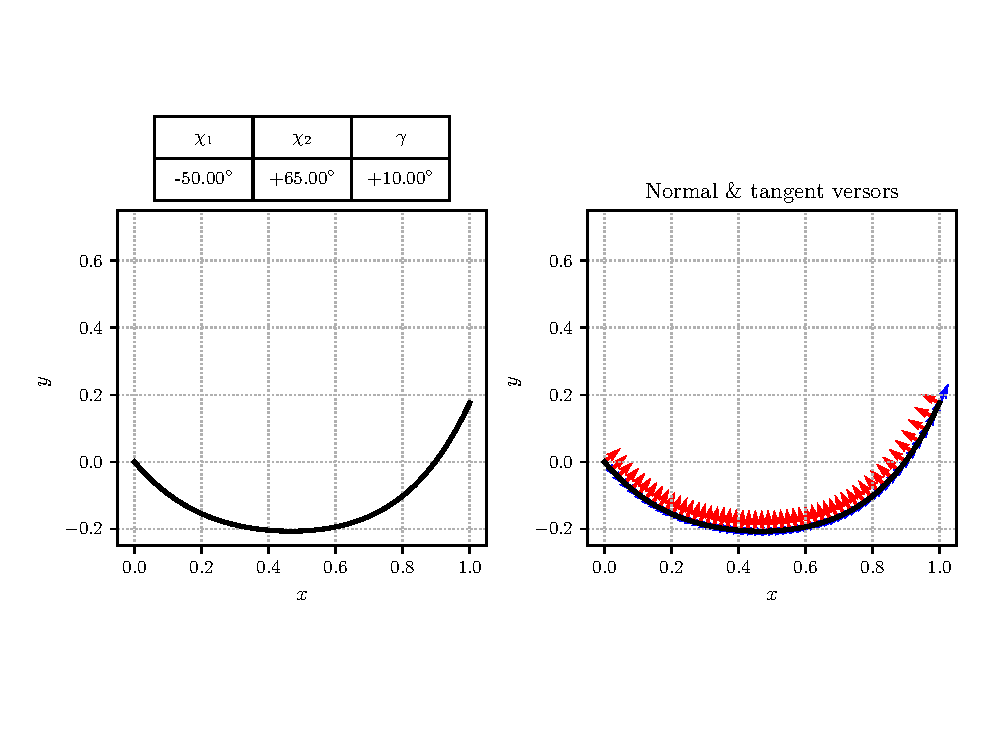
\includegraphics[width=1\linewidth, trim=0cm 1.5cm 0cm 1cm, clip]{pyFigure/figures/cLine1.eps}
  \caption{Camberline: $\gamma = 10^{\circ}$, $\chi_1 = -50^{\circ}$, and $\chi_2 = 65^{\circ}$.}
  \label{fig:cLine1}
\end{figure}

\begin{figure}[!h]
  \centering
  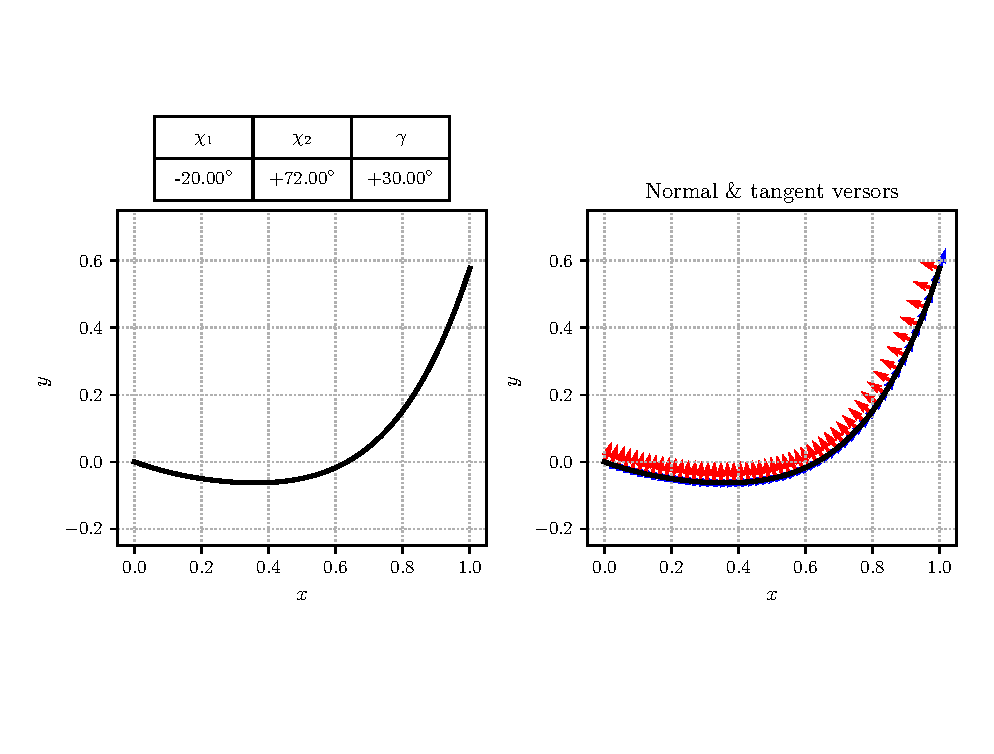
\includegraphics[width=1\linewidth, trim=0cm 1.5cm 0cm 1cm, clip]{pyFigure/figures/cLine2.eps}
  \caption{Camberline: $\gamma = 30^{\circ}$, $\chi_1 = -20^{\circ}$, and $\chi_2 = 70^{\circ}$.}
  \label{fig:cLine2}
\end{figure}

The normal and tangent vectors are employed for the thickness distribution along the camberline, as explained in Section~\ref{sec:profileLine}.

\subsection{Profile Line}
\label{sec:profileLine}

The profile line defines both the \textbf{suction side} and the \textbf{pressure side} of the blade. Utilizing \textbf{Kulfan's parametrization} \cite{kulfan2008universal}, it is possible to generate a wide array of blades \textbf{using just a few parameters}. The preference for parametrization over coordinate-based representation arises from:

\begin{itemize} 
  \item optimization \textbf{speed} 
  \item the fact that, considering the tool's ultimate purpose, parameters are \textbf{easier to correlate} than a pure coordinate-based representation
\end{itemize}

\subsubsection{Formulation}

The profile line is defined by $N + 1$ parameters: $A_i \text{ for } i = 0:N$. These parameters represent the \textbf{weights} of the \textbf{modes} that characterize the blade.

\paragraph{Bernstein Functions}

The shape modes of the blade are described by the Bernstein functions, denoted as $S_{(x, i, N)}$:

\begin{equation}
  S_{(x, i, N)} = A_i \cdot \frac{N!}{(N - i)! \cdot i!} \cdot x^i \cdot (1 - x)^{N - 1} \text{, for } i = 0:N
  \label{eqn:bernstein}
\end{equation}

The blade geometry modes are visualized in Figure~\ref{fig:bernstein}.

\begin{figure}[!h]
  \centering
  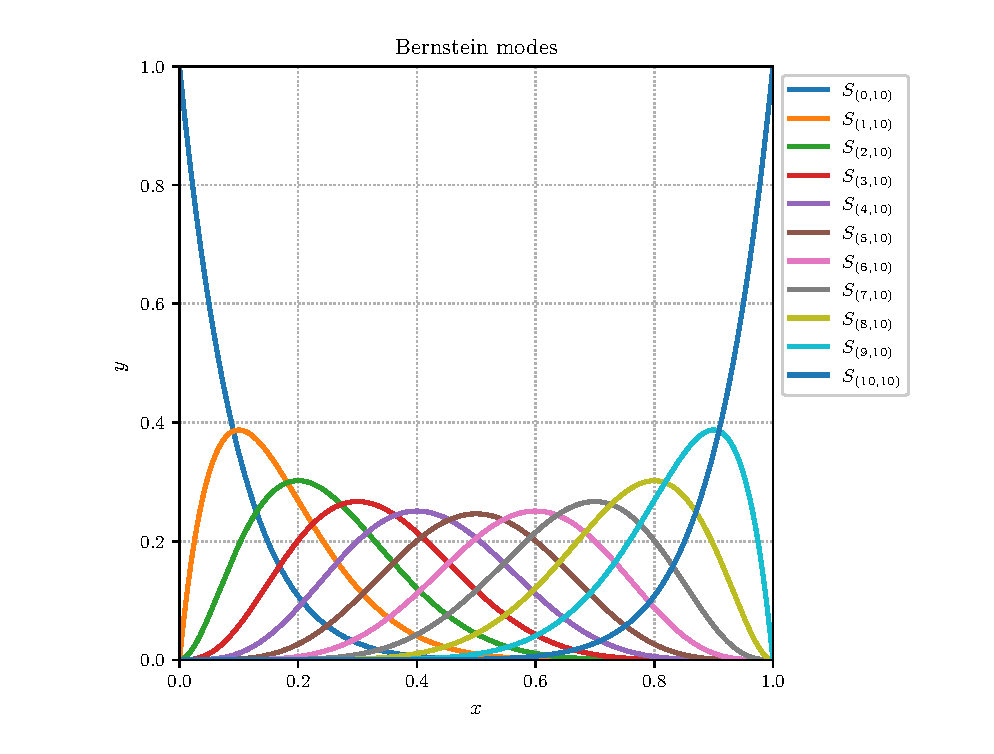
\includegraphics[scale=1]{pyFigure/figures/bernstein.eps}
  \caption{Bernstein function, $S_{(x, i, N)}$, with $A_i = 1$ and $N = 10$.}
  \label{fig:bernstein}
\end{figure}

\paragraph{Shape Function}

In addition to the Bernstein functions as described in Equation~(\ref{eqn:bernstein}), a \textbf{shape function}~\cite{kulfan2010recent} is introduced for representing the \textit{leading edge properties} and \textit{trailing edge properties} of the blade. The shape function, denoted as $C_{(x)}$, takes the form:

\begin{equation}
  C_{(x)} = x^{C_0} \cdot (1 - x)^{C_1}, \text{ where: } C_0 = 0.5 \text{ and } C_1 = 1.0
  \label{eqn:shapeFunction}
\end{equation}

Equation~(\ref{eqn:shapeFunction}) captures the \textit{roundness} of the leading edge and the wedge angle properties at the trailing edge of the blade. The shape function is illustrated in Figure~\ref{fig:shapeFunction}.

\begin{figure}[!h]
  \centering
  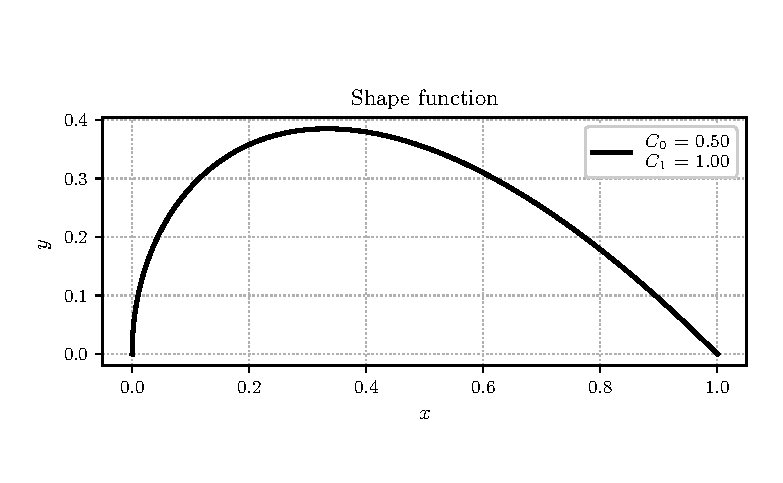
\includegraphics[scale=0.8]{pyFigure/figures/class.eps}
  \caption{Shape function, $C_{(x)}$.}
  \label{fig:shapeFunction}
\end{figure}

\paragraph{Thickness Distribution}

The blade thickness, denoted as $\zeta$, is determined by combining Equation~(\ref{eqn:bernstein}) and Equation~(\ref{eqn:shapeFunction}). Additionally, the trailing edge radius, $R_{TE}$, is incorporated using a linear distribution, $\zeta_{TE}$, over the camberline. The thickness distribution $\zeta_{(x)}$ is related to camberline properties and \textbf{is distributed using a unit Bernstein function} - $S_{(x, 0, 2)}$. The distribution $\zeta_{TE_{(x)}}$ solely relies on camberline properties $n_x$ and $n_y$.

\begin{align}
  \zeta_{(x)}       & = \sum_{i = 0}^N S_{(x, i, N)} \cdot C_{(x)} \\
  \zeta_{TE_{(x)}}  & = x \cdot R_{TE} 
\end{align}

The pressure(suction) side ($\pm$) profile line coordinates are then computed as: 

\begin{align}
  x_{PS/SS} & = x_{camberline} \pm n_x \cdot \zeta_{(x)} \cdot S_{(x, 0, 2)} \pm n_x \cdot \zeta_{TE_{(x)}}\\ 
  y_{PS/SS} & = y_{camberline} \pm n_y \cdot \zeta_{(x)} \cdot S_{(x, 0, 2)} \pm n_y \cdot \zeta_{TE_{(x)}}+ \zeta_{(x)} \cdot \big[1 - S_{(x, 0, 2)}\big]
\end{align}

\begin{figure}[H]
    \centering
    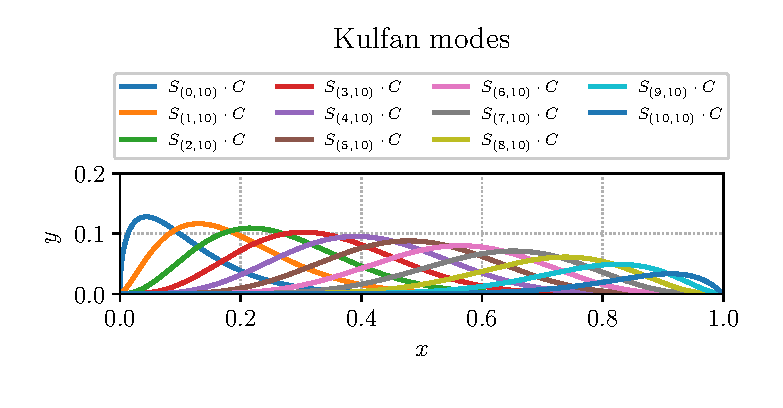
\includegraphics[scale=0.9]{pyFigure/figures/kulfan.eps}
    \caption{Kulfan modes, $S_{(x, i, N)} \cdot C_{(x)}$, with $A_i = 1$ and $N = 10$.}
    \label{fig:kulfan}
\end{figure}

Figures~\ref{fig:kulfan} presents the \textbf{profile blade modes}, which are a combination of Equation~(\ref{eqn:bernstein}) and Equation~(\ref{eqn:shapeFunction}).

The suction side and pressure side coordinates are computed using a \textit{custom set of points} over the camberline.
The camberline is discretized with \textbf{Chebyshev nodes} all along the chord. This approximation allows better accuracy at the leading edge and at the traling edge of the blade.

Figure~\ref{fig:bladeNodes} and Figure~\ref{fig:bladeNodes1} show clearly the blade coordinates starting from the chord discretization passing through the camberline discretization to the suction side and pressure side points.
Using the \textbf{Chebyshev nodes} allows having a \textbf{faster generation} of the blade while keeping \textbf{good accuracy} over the blade coordinates representation. 

\begin{figure}[H]
  \centering
  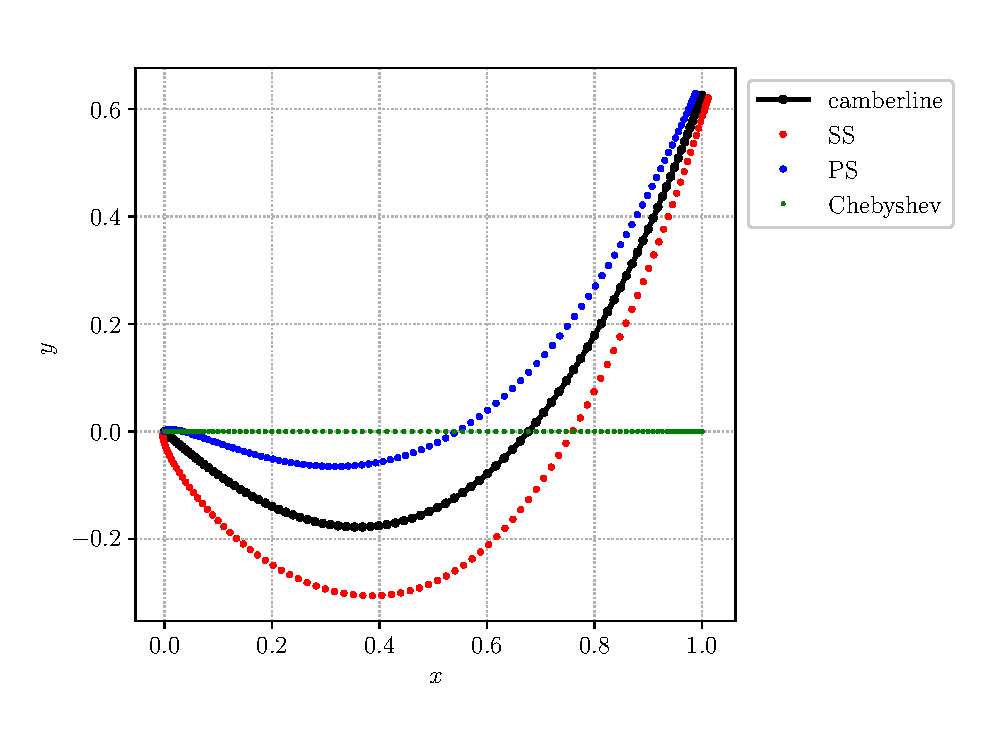
\includegraphics[scale=0.5]{pyFigure/figures/coordinate1.eps}
  \caption{Coordinate based representation of the blade.}
  \label{fig:bladeNodes}
\end{figure}

\begin{figure}[H]
  \centering
  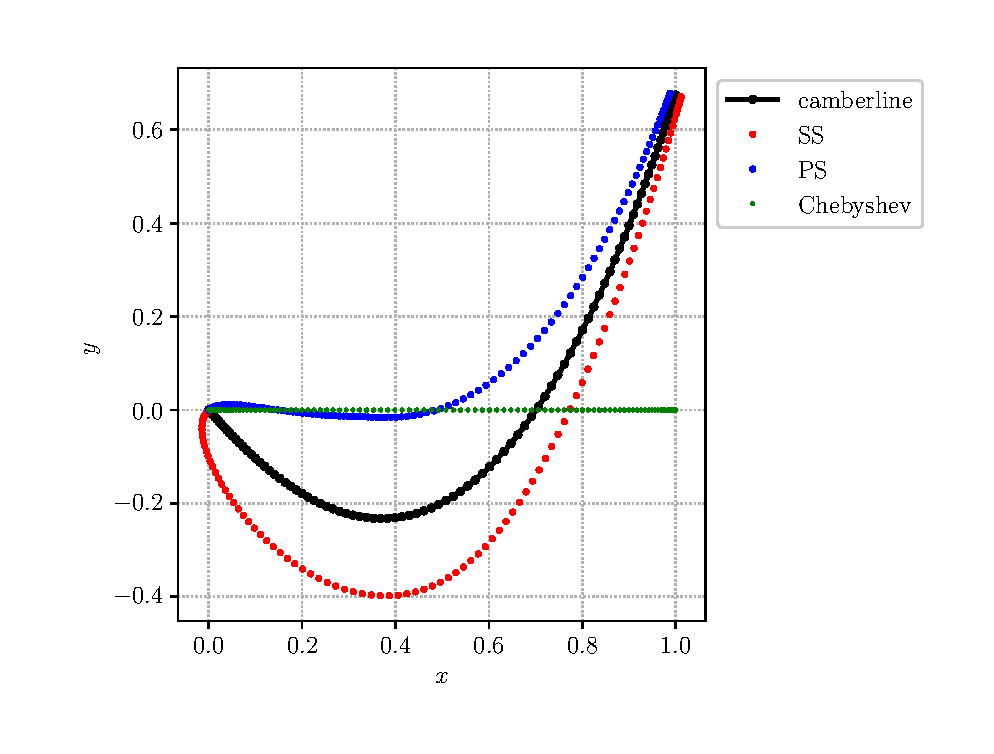
\includegraphics[scale=0.5]{pyFigure/figures/coordinate2.eps}
  \caption{Coordinate based representation of the blade.}
  \label{fig:bladeNodes1}
\end{figure}

\subsubsection{Main Features}

Kulfan's parametrization retains several crucial geometric properties:

\begin{itemize}
  \item The leading edge radius, $R_{LE}$, is determined solely by the $A_0$ parameter \cite[App. B]{kulfan2008universal}. $A_0 = \sqrt{2 \cdot R_{LE}}$.
  \item The trailing edge angle, $\beta$, is directly related to the $A_{N}$ parameter \cite[App. A]{kulfan2008universal}. $A_N = tan(\beta) + R_{TE}$.
\end{itemize}

These features hold great \textbf{significance} in studying the \textbf{blade characteristics} in relation to flow properties.

\subsubsection{Scaling}

The blade optimization takes place through \textbf{incremental steps}, utilizing a strategy that ensures \textit{faster convergence}. One key aspect of this strategy is to perform a \textbf{scaling} of the blade once convergence is achieved. 
This step is crucial for optimizing a blade with many degrees of freedom. 
The primary aim of scaling is to address potential \textit{pits} within the domain during the blade optimization.

This scaling is generated solving a linear system. The linear system uses a matrix of $N_{new} \ \times \ N_{new}$ dimension. 
To build up this matrix, the blade, parametrized with lower number of parameters $N$, is evaluated on an equispaced number of points, $N_{new}$ times, along the axial chord.  
The resulting matrix is then used to compute the new parametrization, made by $N_{new}$ parameters.

It's important to note that the only unaltered parameters are:

\begin{itemize}
    \item For the suction side and pressure side: $R_{LE}$ and $\beta$
    % \item For the pressure side: $R_{LE}$ and $\beta$
    \item For the camberline: $\chi_1$, $\chi_2$ and $\gamma$
    % \item $A_0$ \& $A_i$ for the suction side and the pressure side 
    % \item $A_0$ 
    % \item $A_i$ 
    % \item $\chi_1$
    % \item $\chi_2$
\end{itemize}

These parameters remain unchanged during the scaling process due to their direct correlation with the blade's geometrical properties

Figures~\ref{fig:blade01} and~\ref{fig:blade03} illustrate different blades and the outcomes resulting from their scaling.

\begin{figure}[H]
  \centering
  \hspace*{-3cm}
  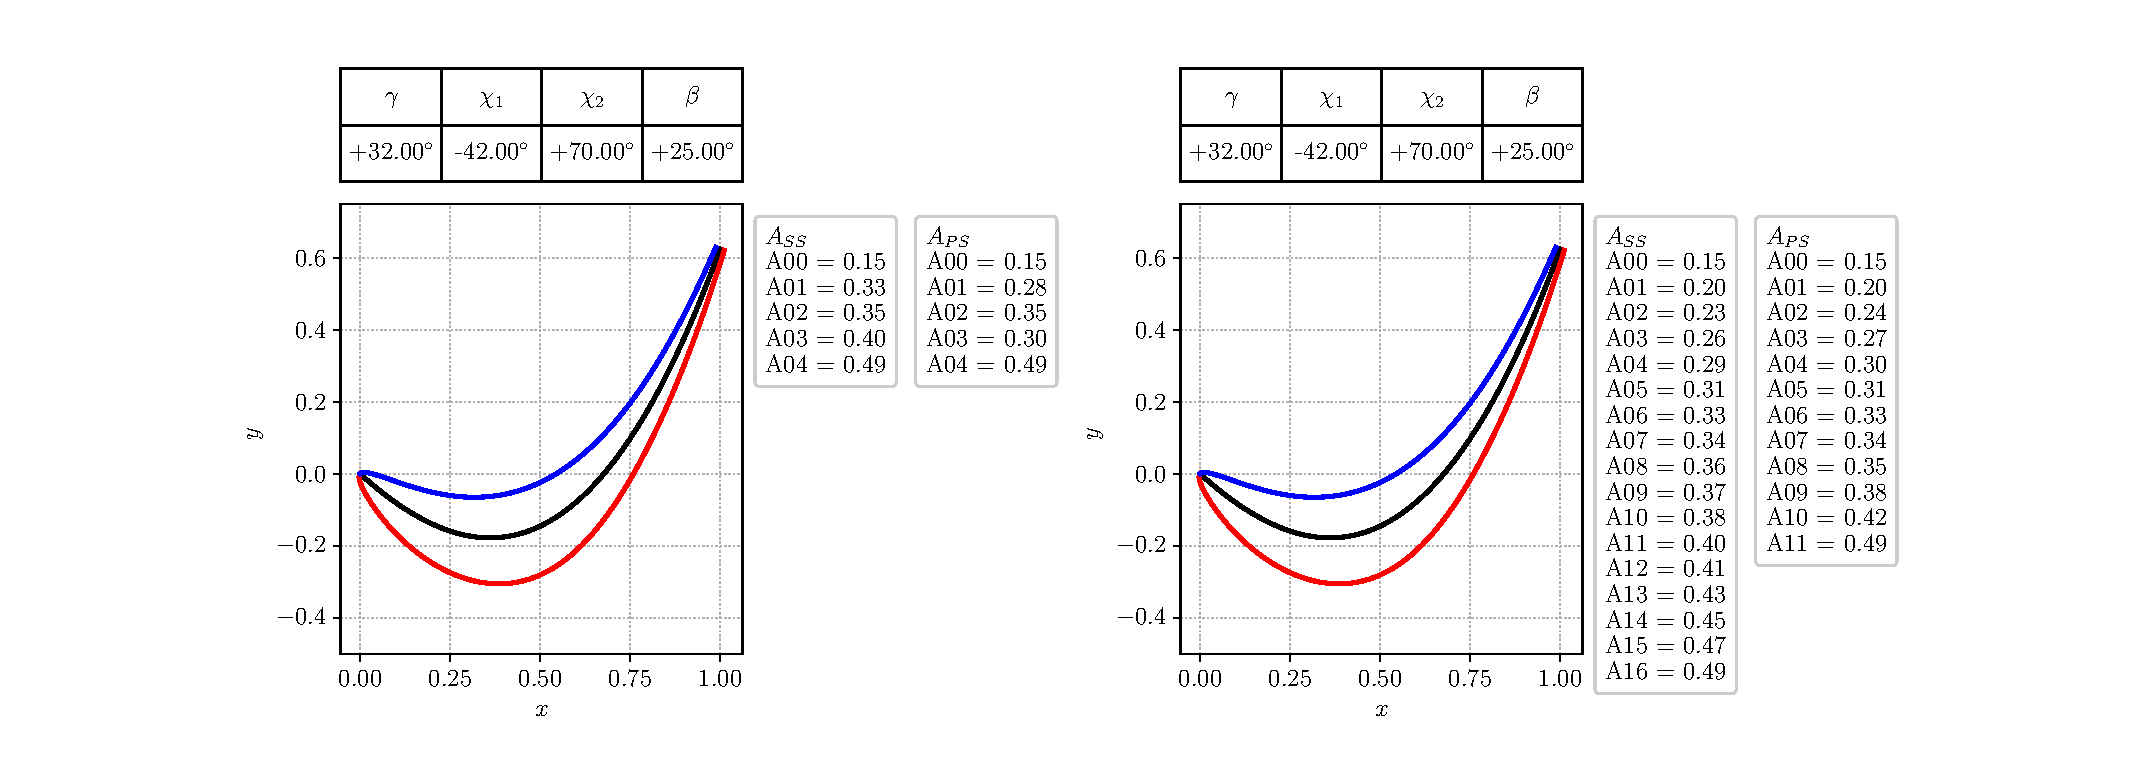
\includegraphics[width=1.35\textwidth]{pyFigure/figures/blade1.eps}
  \caption{Example No. 1 of blade scaling following Kulfan's parametrization.}
  \label{fig:blade01}
\end{figure}

\begin{figure}[H]
  \centering
  \hspace*{-3cm}
  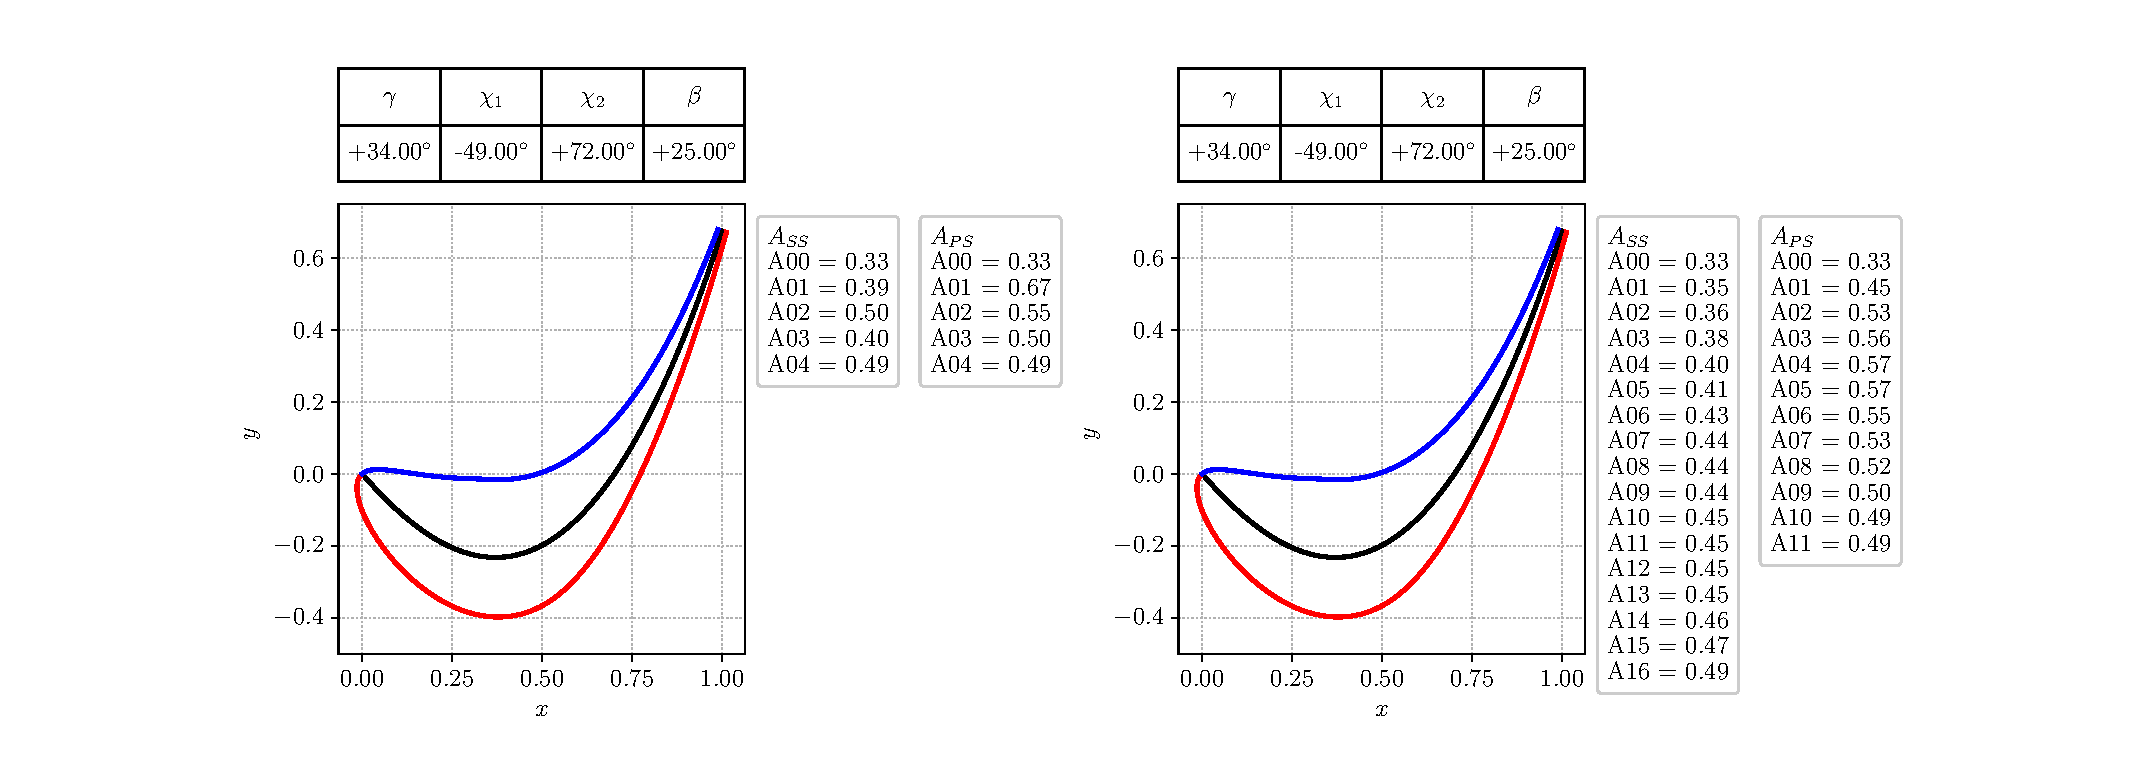
\includegraphics[width=1.35\textwidth]{pyFigure/figures/blade2.eps}
  \caption{Example No. 2 of blade scaling following Kulfan's parametrization.}
  \label{fig:blade03}
\end{figure}

\section{Aerodynamic Style Parametrization}
\label{sec:aeroStyle}

In contrast to the \textbf{aerodynamic duty}, the \textbf{aerodynamic style} allows to define locally the load distribution along the blade. 

The \textbf{aerodynamic style} is defined by the Mach fraction, $\frac{M}{M_{TE}}$, over the surface length fraction, $\frac{S}{S_{TOT}}$. 

There are multiple \textit{reasons} about the use of these parameters. The key ones are:

\begin{itemize}
  \item The leading edge is a regione where, due to the high curvature of the geometry, there is a \textbf{high change in surface fraction over the axial chord}. Since this region is a very important for the correlation study, the $\frac{M}{M_{TE}} \ vs \ \frac{S}{S_{TOT}}$ formulation results appropriate.
  \item The \textbf{boundary layer} properties, such as transition and detachament, is mostly dependent on the \textbf{total flow path length} done by the flow - described by $S$ - and not over its projection over the axis - described by $x$.
\end{itemize}

The \textbf{aerodynamic style}~\cite{clark2019step} is defined by these variables:

\begin{itemize}
  \item $\frac{M_{LE}}{M_{TE}} \frac{M_2}{M_1}$: leading edge Mach fraction. This parameter defines the load at the leading edge on the suction side.
  \item $\frac{M_{PEAK}}{M_{TE}}$: peak Mach fraction. Defines the peak Mach fraction on the suction side, representing the highest Mach value over the blade.
  \item $\frac{M_{PRESS}}{M_{TE}} \frac{M_2}{M_{1, ax}}$: pressure Mach number. It is a \textbf{double descriptor} of the leading edge load on the suction side and the Mach fraction before the Mach fraction raises to reach the trailing edge on the pressure side. 
  \item $\frac{S_{PEAK}}{S_{TOT}}$: surface fraction position where the peak Mach fraction, $\frac{M_{PEAK}}{M_{TE}}$, is positioned over the load distribution.
\end{itemize}

It is important to understand that \textbf{the load varies with respect to $\frac{M_1}{M_2}$ and $\frac{M_{1, ax}}{M_2}$}. This
is due to the fact that the leading edge load distribution is highly sensitive to the inlet flow properties\footnote{Defined by $M_1$ and $\alpha_1$.}. 

\subsection{Trial \& Error}

Having introduced the variables which define the loading distribution, it is important to notice that these variables have to 
be tuned in order to meet the manufacturing requirements - such as the leading edge radius ($\frac{R_{LE}}{c} \geq 1.25 \cdot 10^{-2}$).
The trailing edge radius ($\frac{R_{TE}}{c}$) is set at $1.25 \cdot 10^{-2}$ throughout the whole study. These values are dictated mainly by the manufacturing capabilities in the turbomachinery industry. 

This concept is very important because there are blades which might not satisfy both the aerodynamic style and the duty imposed.
The trial and error tuning of the loading behavior at the leading edge can be seen as a design limit but it can be also seen as a first \textit{filtering operation} 
over the aerodynamic style and the aerodynamic duty for appreciable results.

The \textbf{\textit{trial and error}} approach has been used mainly over the loading behavioiur at the leading edge 
- both at the suction side and the pressure side of the blade. These corrections are mainly made on the behavior of the 
conjunction point between the ellipse shaped loading at the leading edge with the straight line after it. 

This behavior is of paramount importance as it enables the convergence of a specific blade
set in terms of loading distribution and the exit flow angle.

Figures~\ref{fig:aerodynamicStyle} provide visualizations of the load properties obtained using a \textbf{spline parametrization}:

\begin{figure}[H]
  \centering
  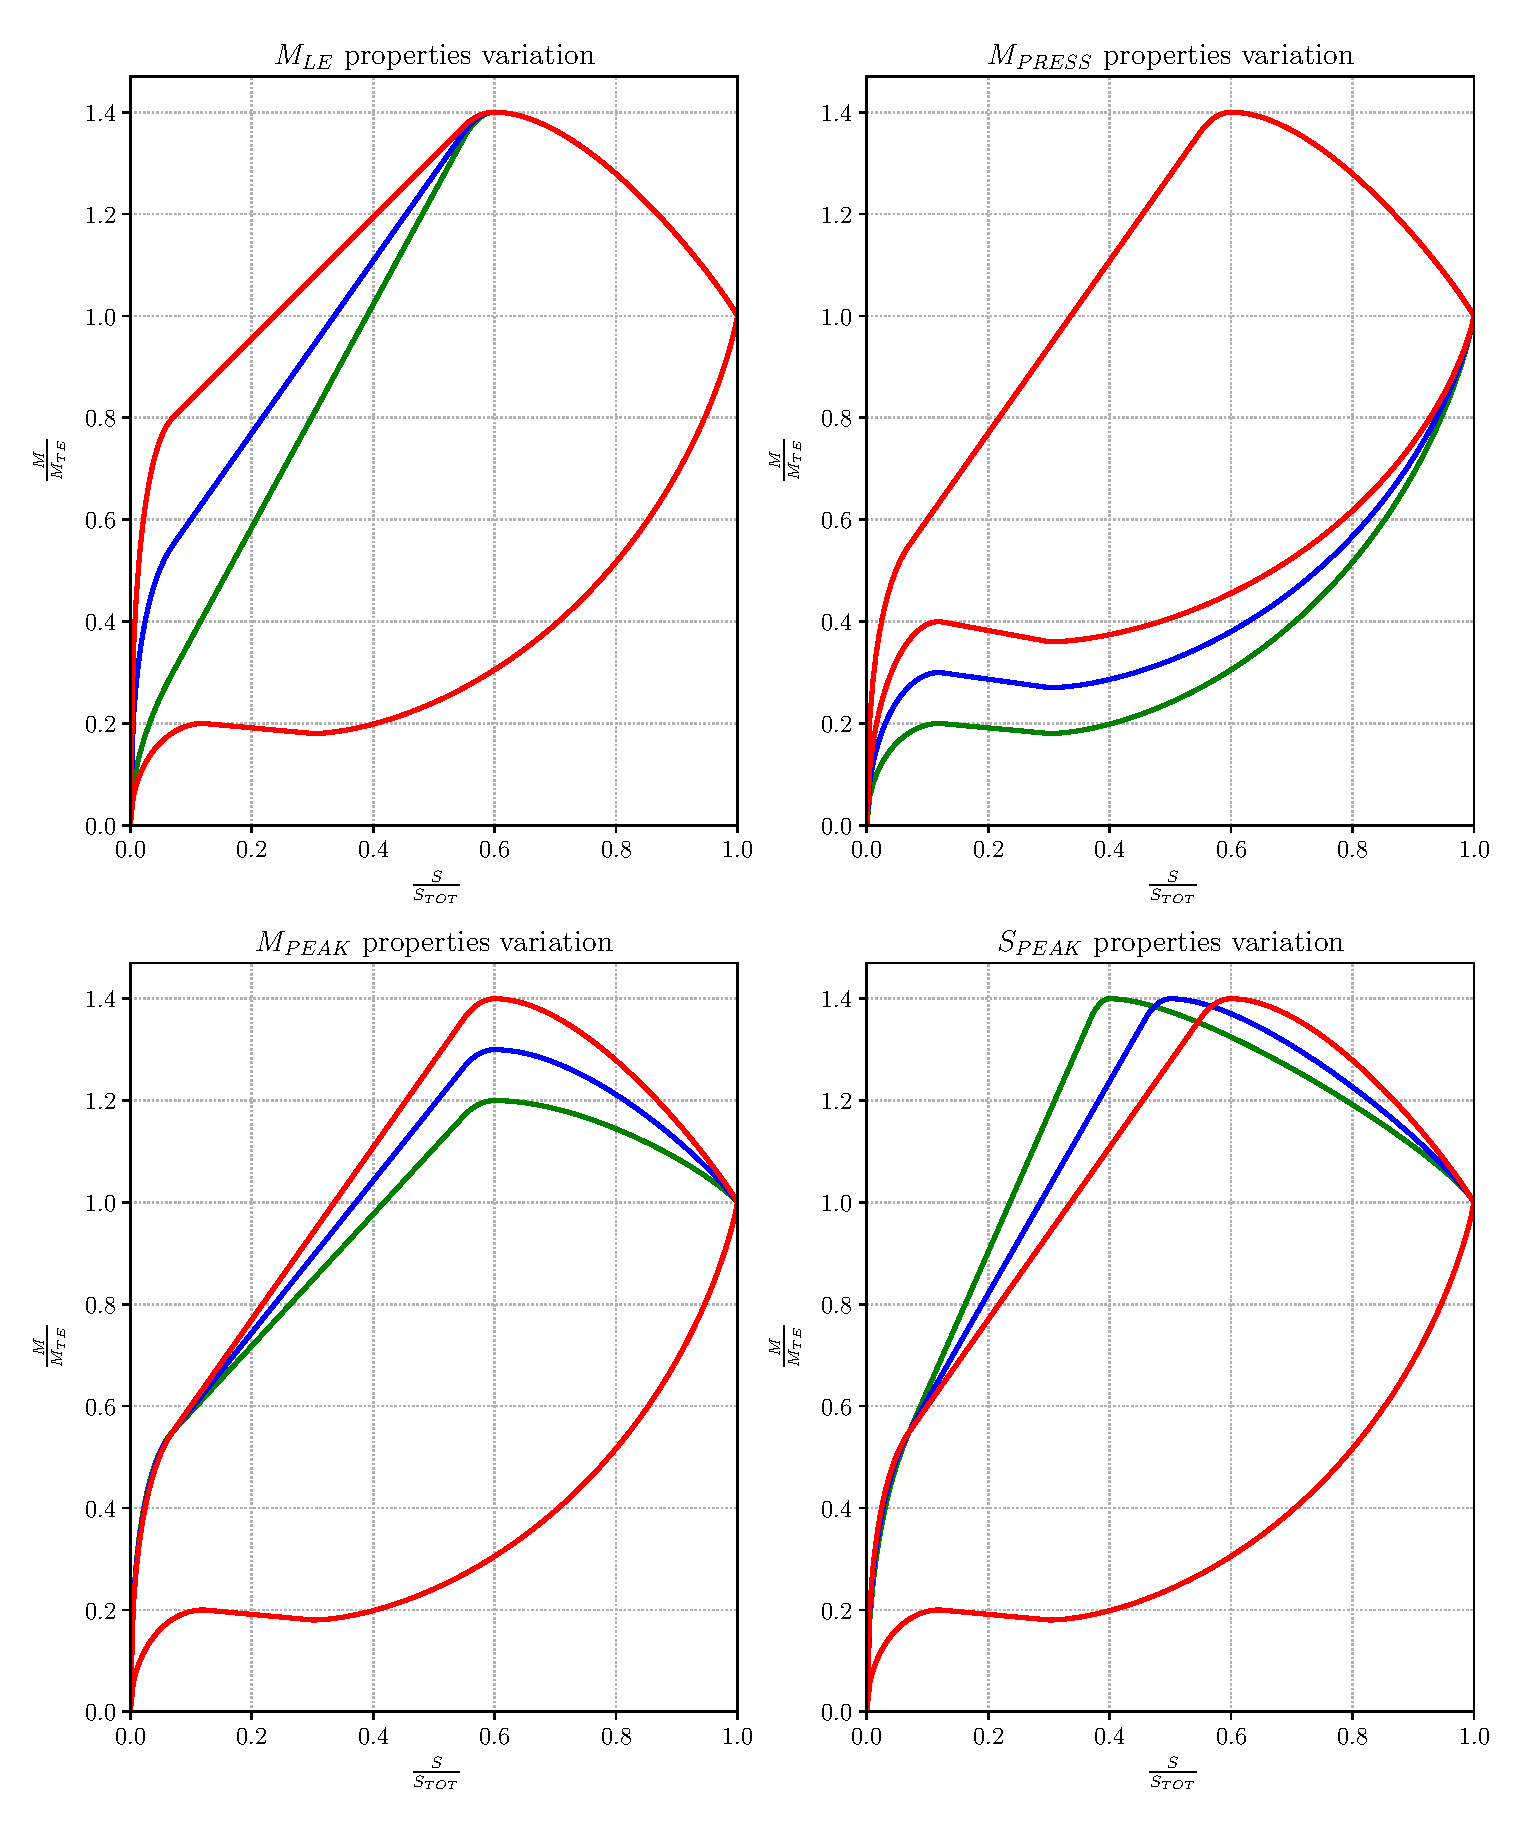
\includegraphics[scale=0.5]{pyFigure/figures/loadProperties.eps}
  \caption{Aerodynamic style properties.}
  \label{fig:aerodynamicStyle}
\end{figure}

% \begin{frame}{Flow solver}
    \texttt{MISES} is based on a \textbf{Newton's method optimizer}. Giving geometry and constraints, the solver computes the blade channel flow. 
    % \\ [0.5cm]
    The solver relies on:
    \begin{align*}
        \text{\textbf{Momentum equation}: }\mathcal{R}_1 & = \Delta p + \frac{m}{A} \Delta \tilde{q} - P_s - p \ \Delta \mathcal{P} = 0 \\
        \text{\textbf{Entropy equation}: }\mathcal{R}_2 & = p \ \Delta \log{\tilde{p}_{0, a}} - p \ \Delta \mathcal{P} = 0
    \end{align*}
    These 2 models are \textbf{blended} into one single equation:
    \begin{equation*}
        \mathnormal{g} \cdot \mathcal{R}_1 + (1 - \mathnormal{g}) \cdot \mathcal{R}_2 = 0
    \end{equation*}
    Where $\mathnormal{g}$ takes into account the local changes of \textbf{total pressure} and the \textbf{velocity gradients}.
    \\ [0.5cm]
    The solver models the boundary layer using \textbf{interchangeably} the $\boldsymbol{e^n}$ and \textbf{Abu-Ghannam-Shaw} models.
\end{frame}

\begin{frame}{\texttt{MISES} - Geometry, BCs \& control points}
    \vspace{-3cm}
    \begin{columns}
        \column{0.5\textwidth}
        \vspace{2cm}
        \begin{figure}
            \centering
            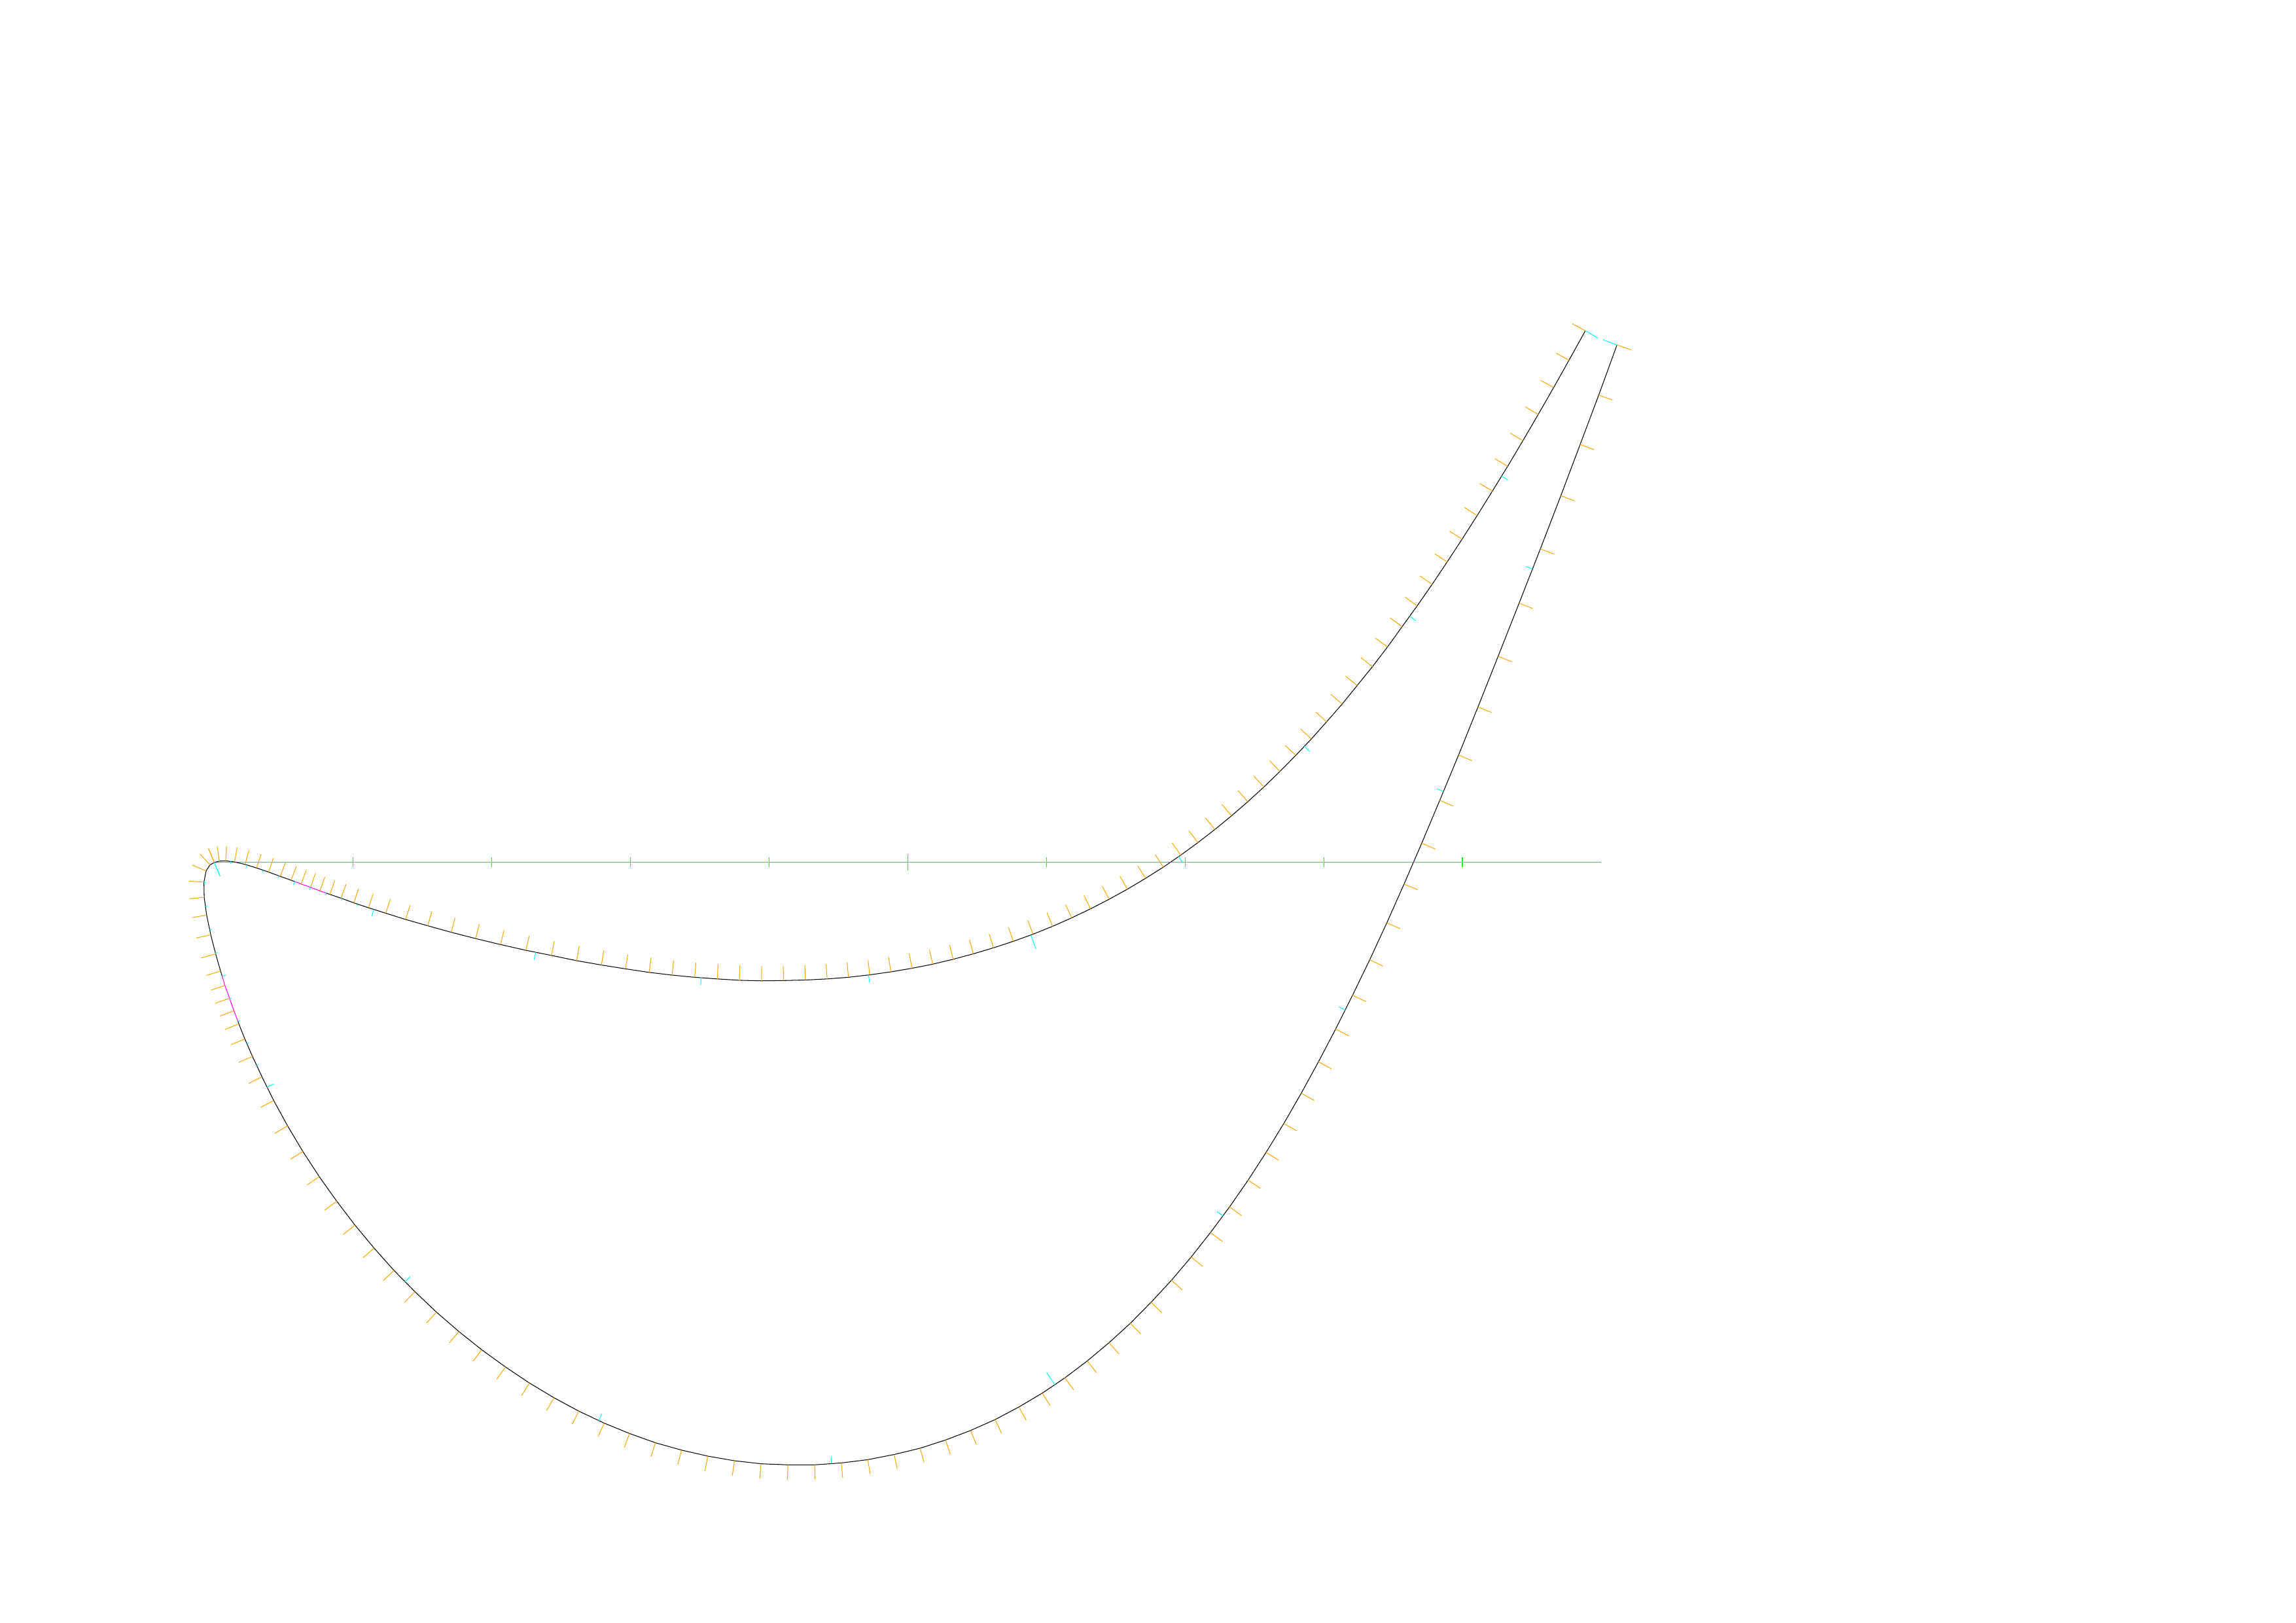
\includegraphics[scale=0.3]{./images/datablade120-2.png}
        \end{figure}
        \column{0.5\textwidth}
        \begin{figure}
            \centering
            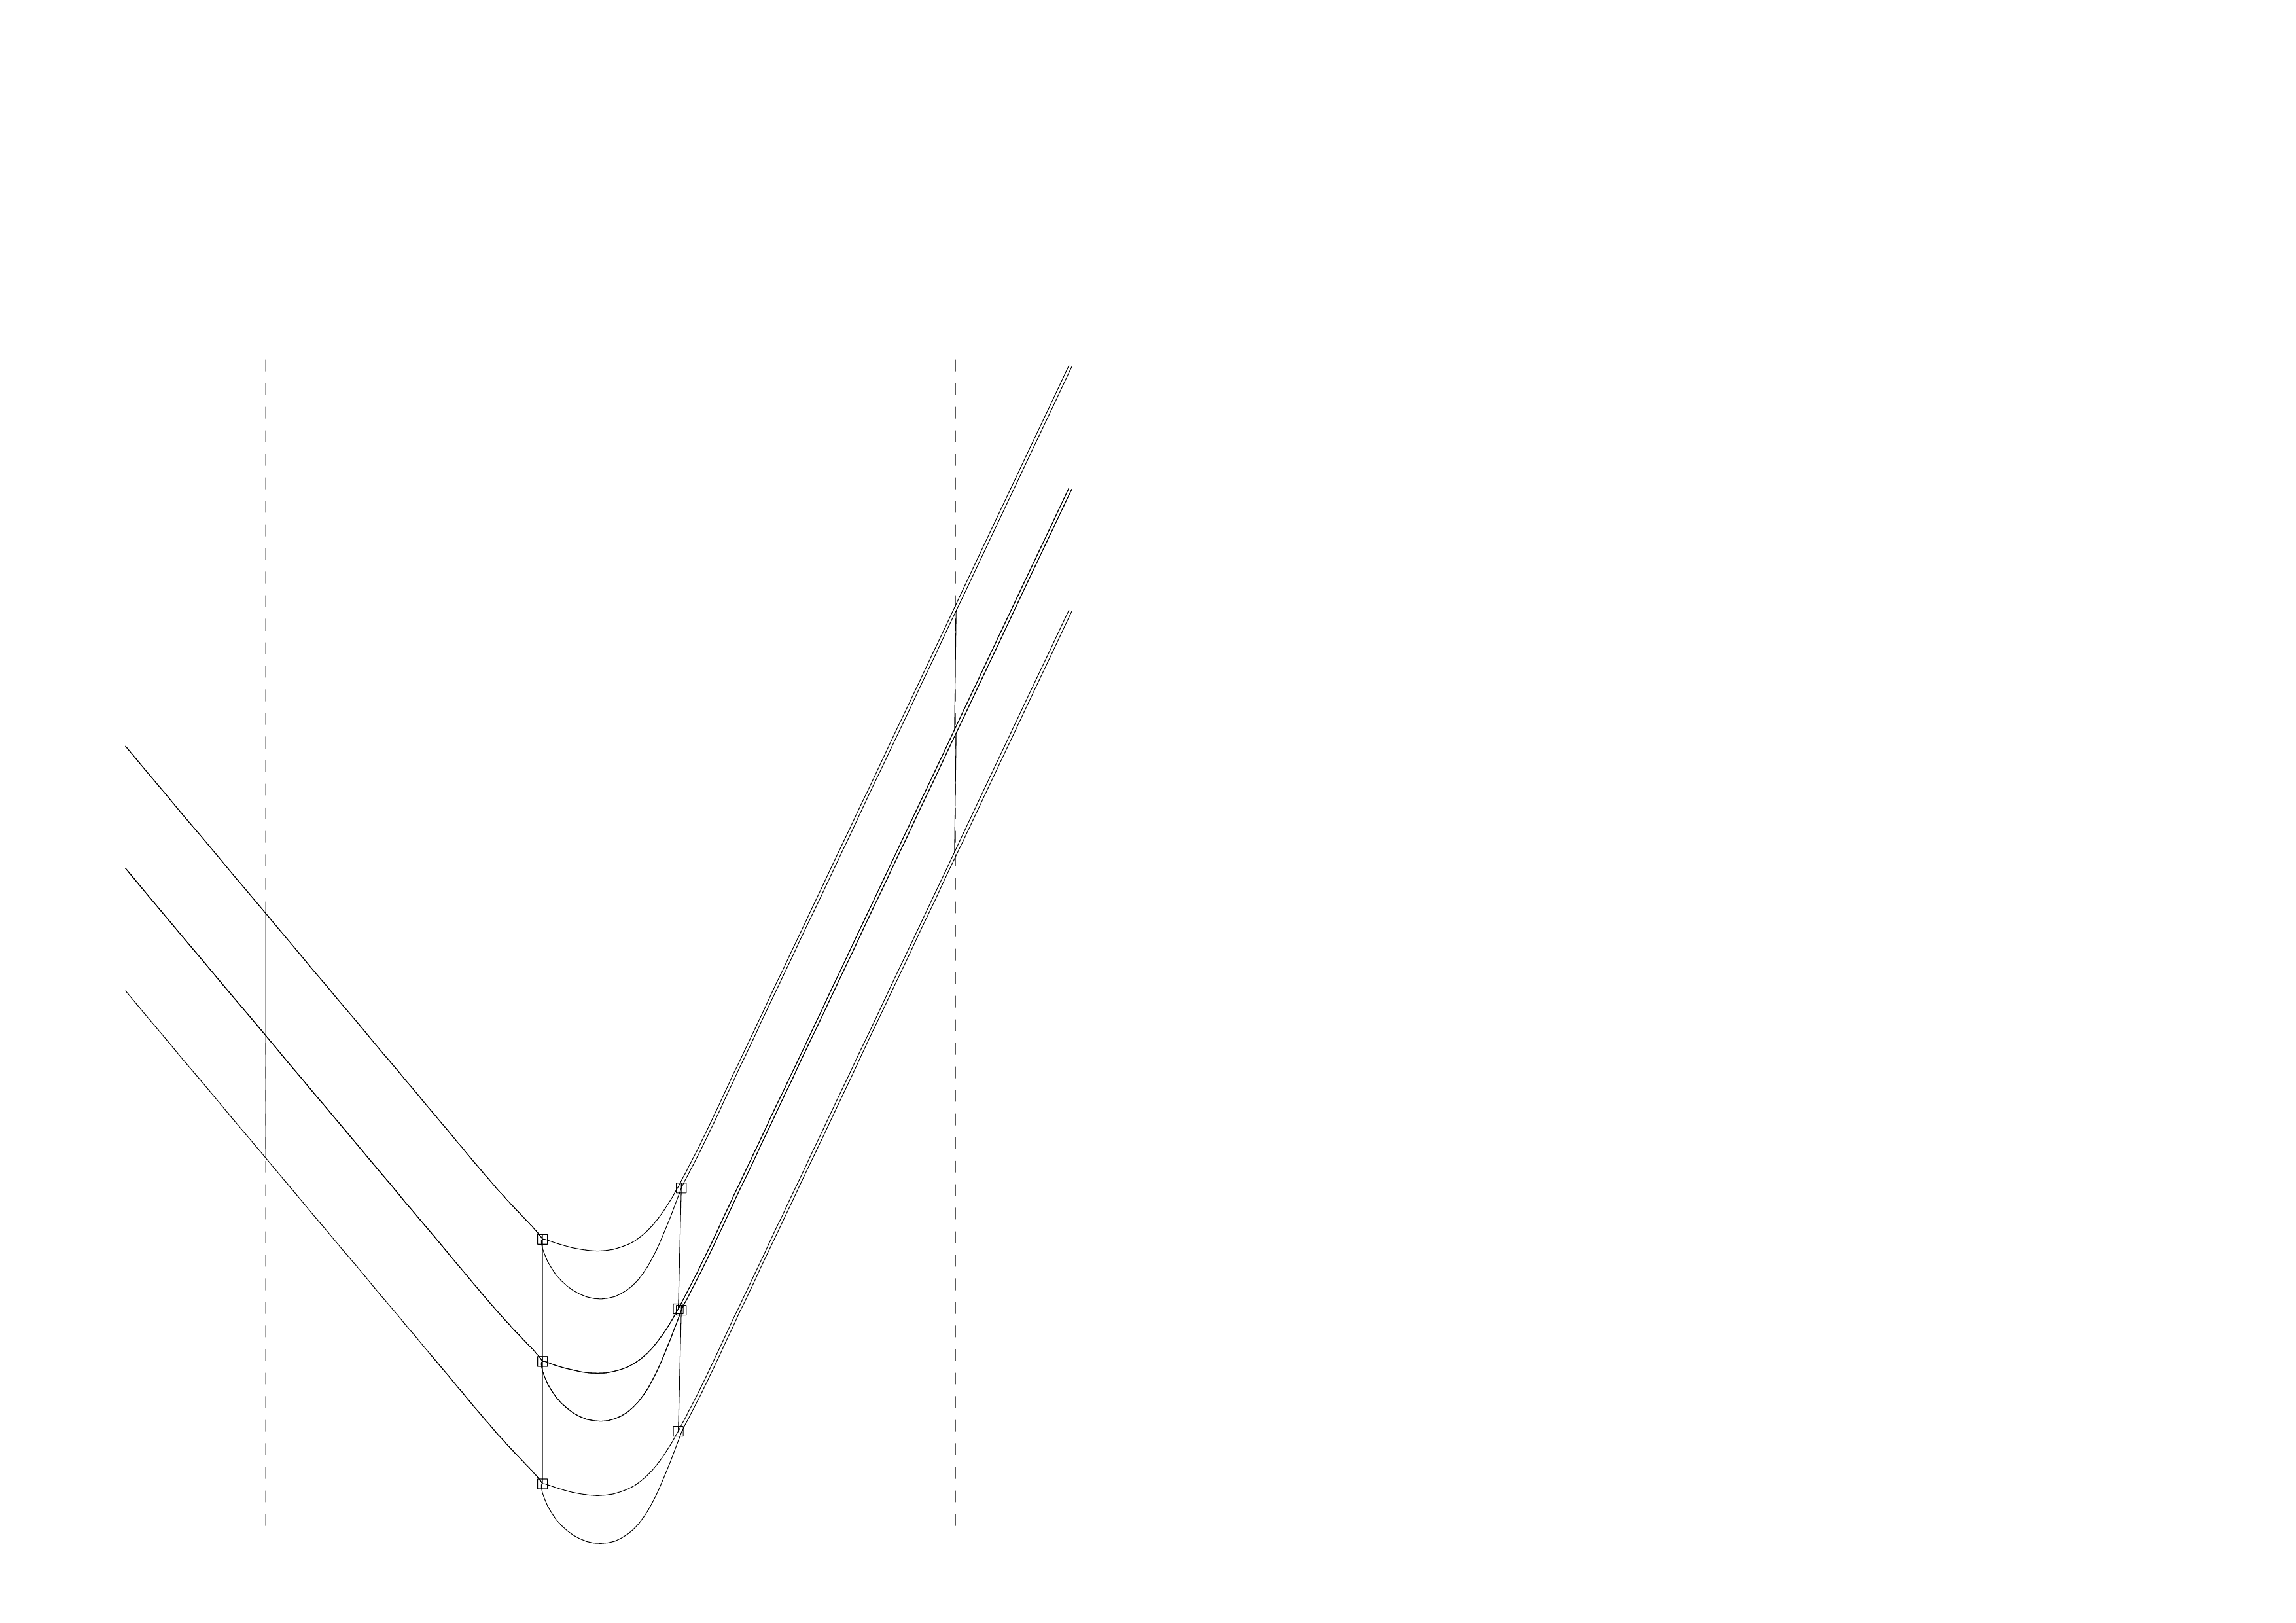
\includegraphics[scale=0.4]{./images/datablade120-1.png}
        \end{figure}
    \end{columns}
\end{frame}

\begin{frame}{\texttt{MISES} - Grid \& flow}
    \vspace{-2.5cm}
    \begin{columns}
        \column{0.5\textwidth}
        \vspace{0.5cm}
        \begin{figure}
            \centering
            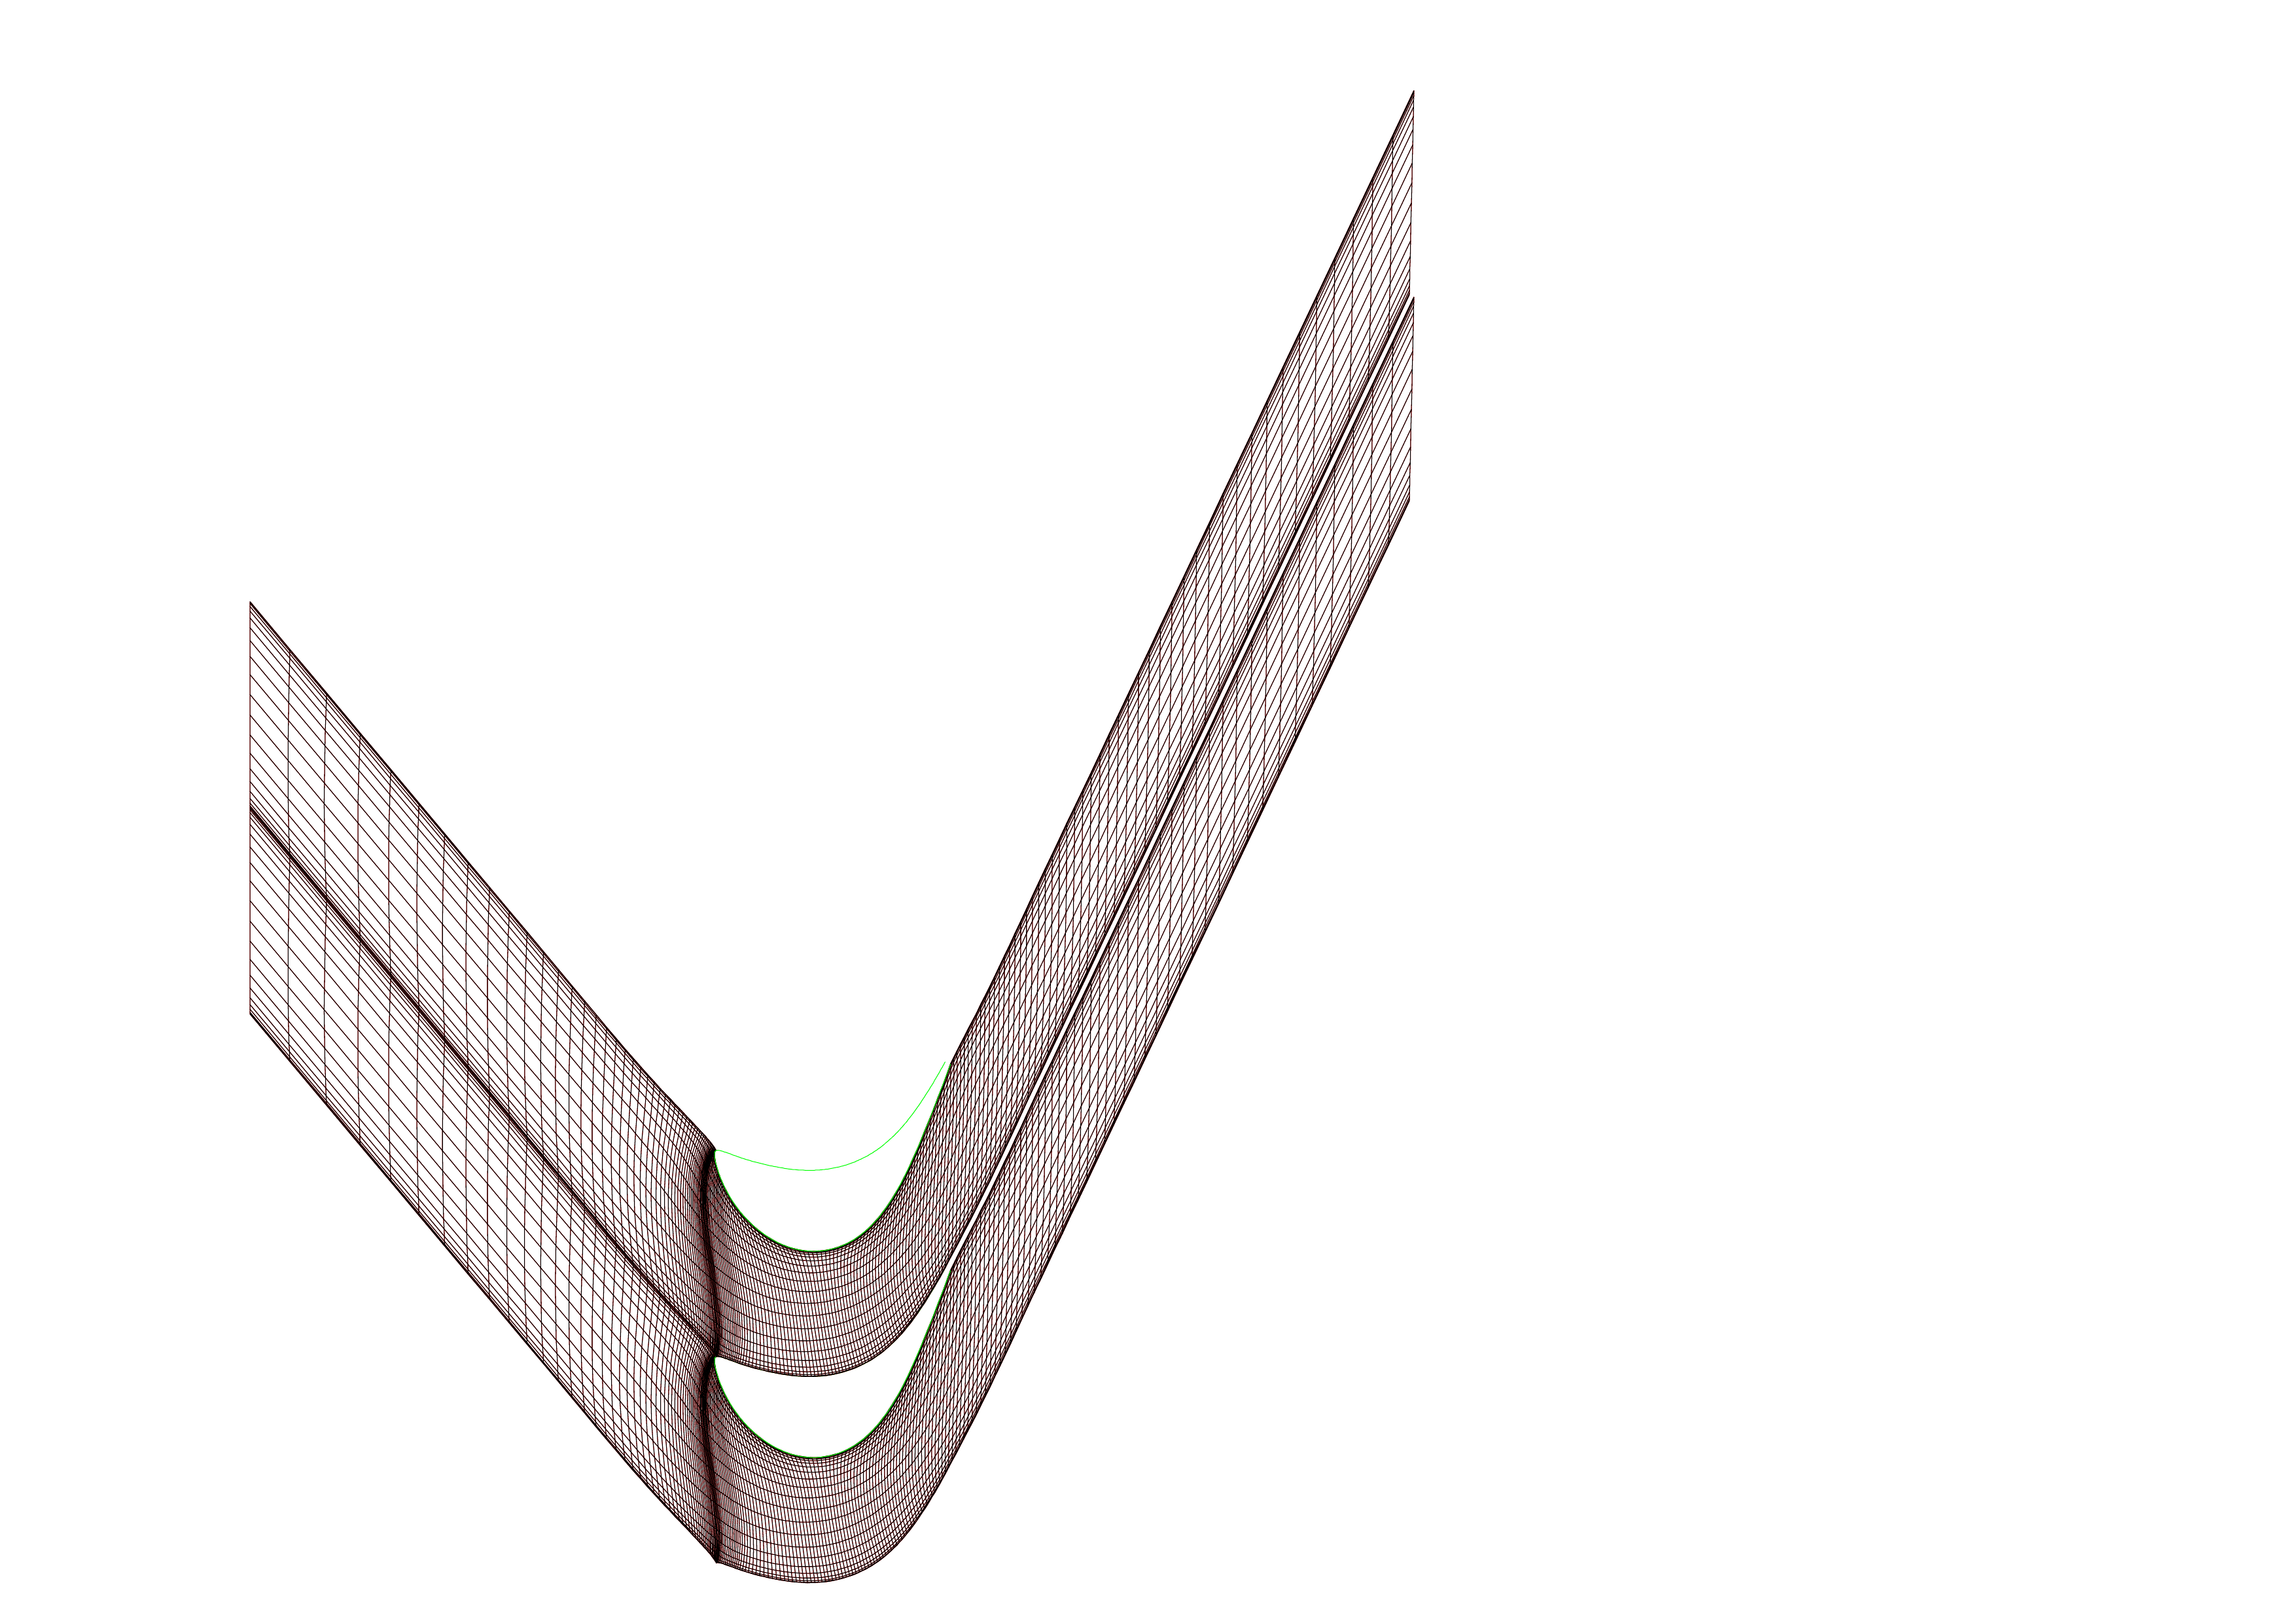
\includegraphics[scale=0.4]{./images/datablade120-3.png}
        \end{figure}
        \column{0.5\textwidth}
        \begin{figure}
            \centering
            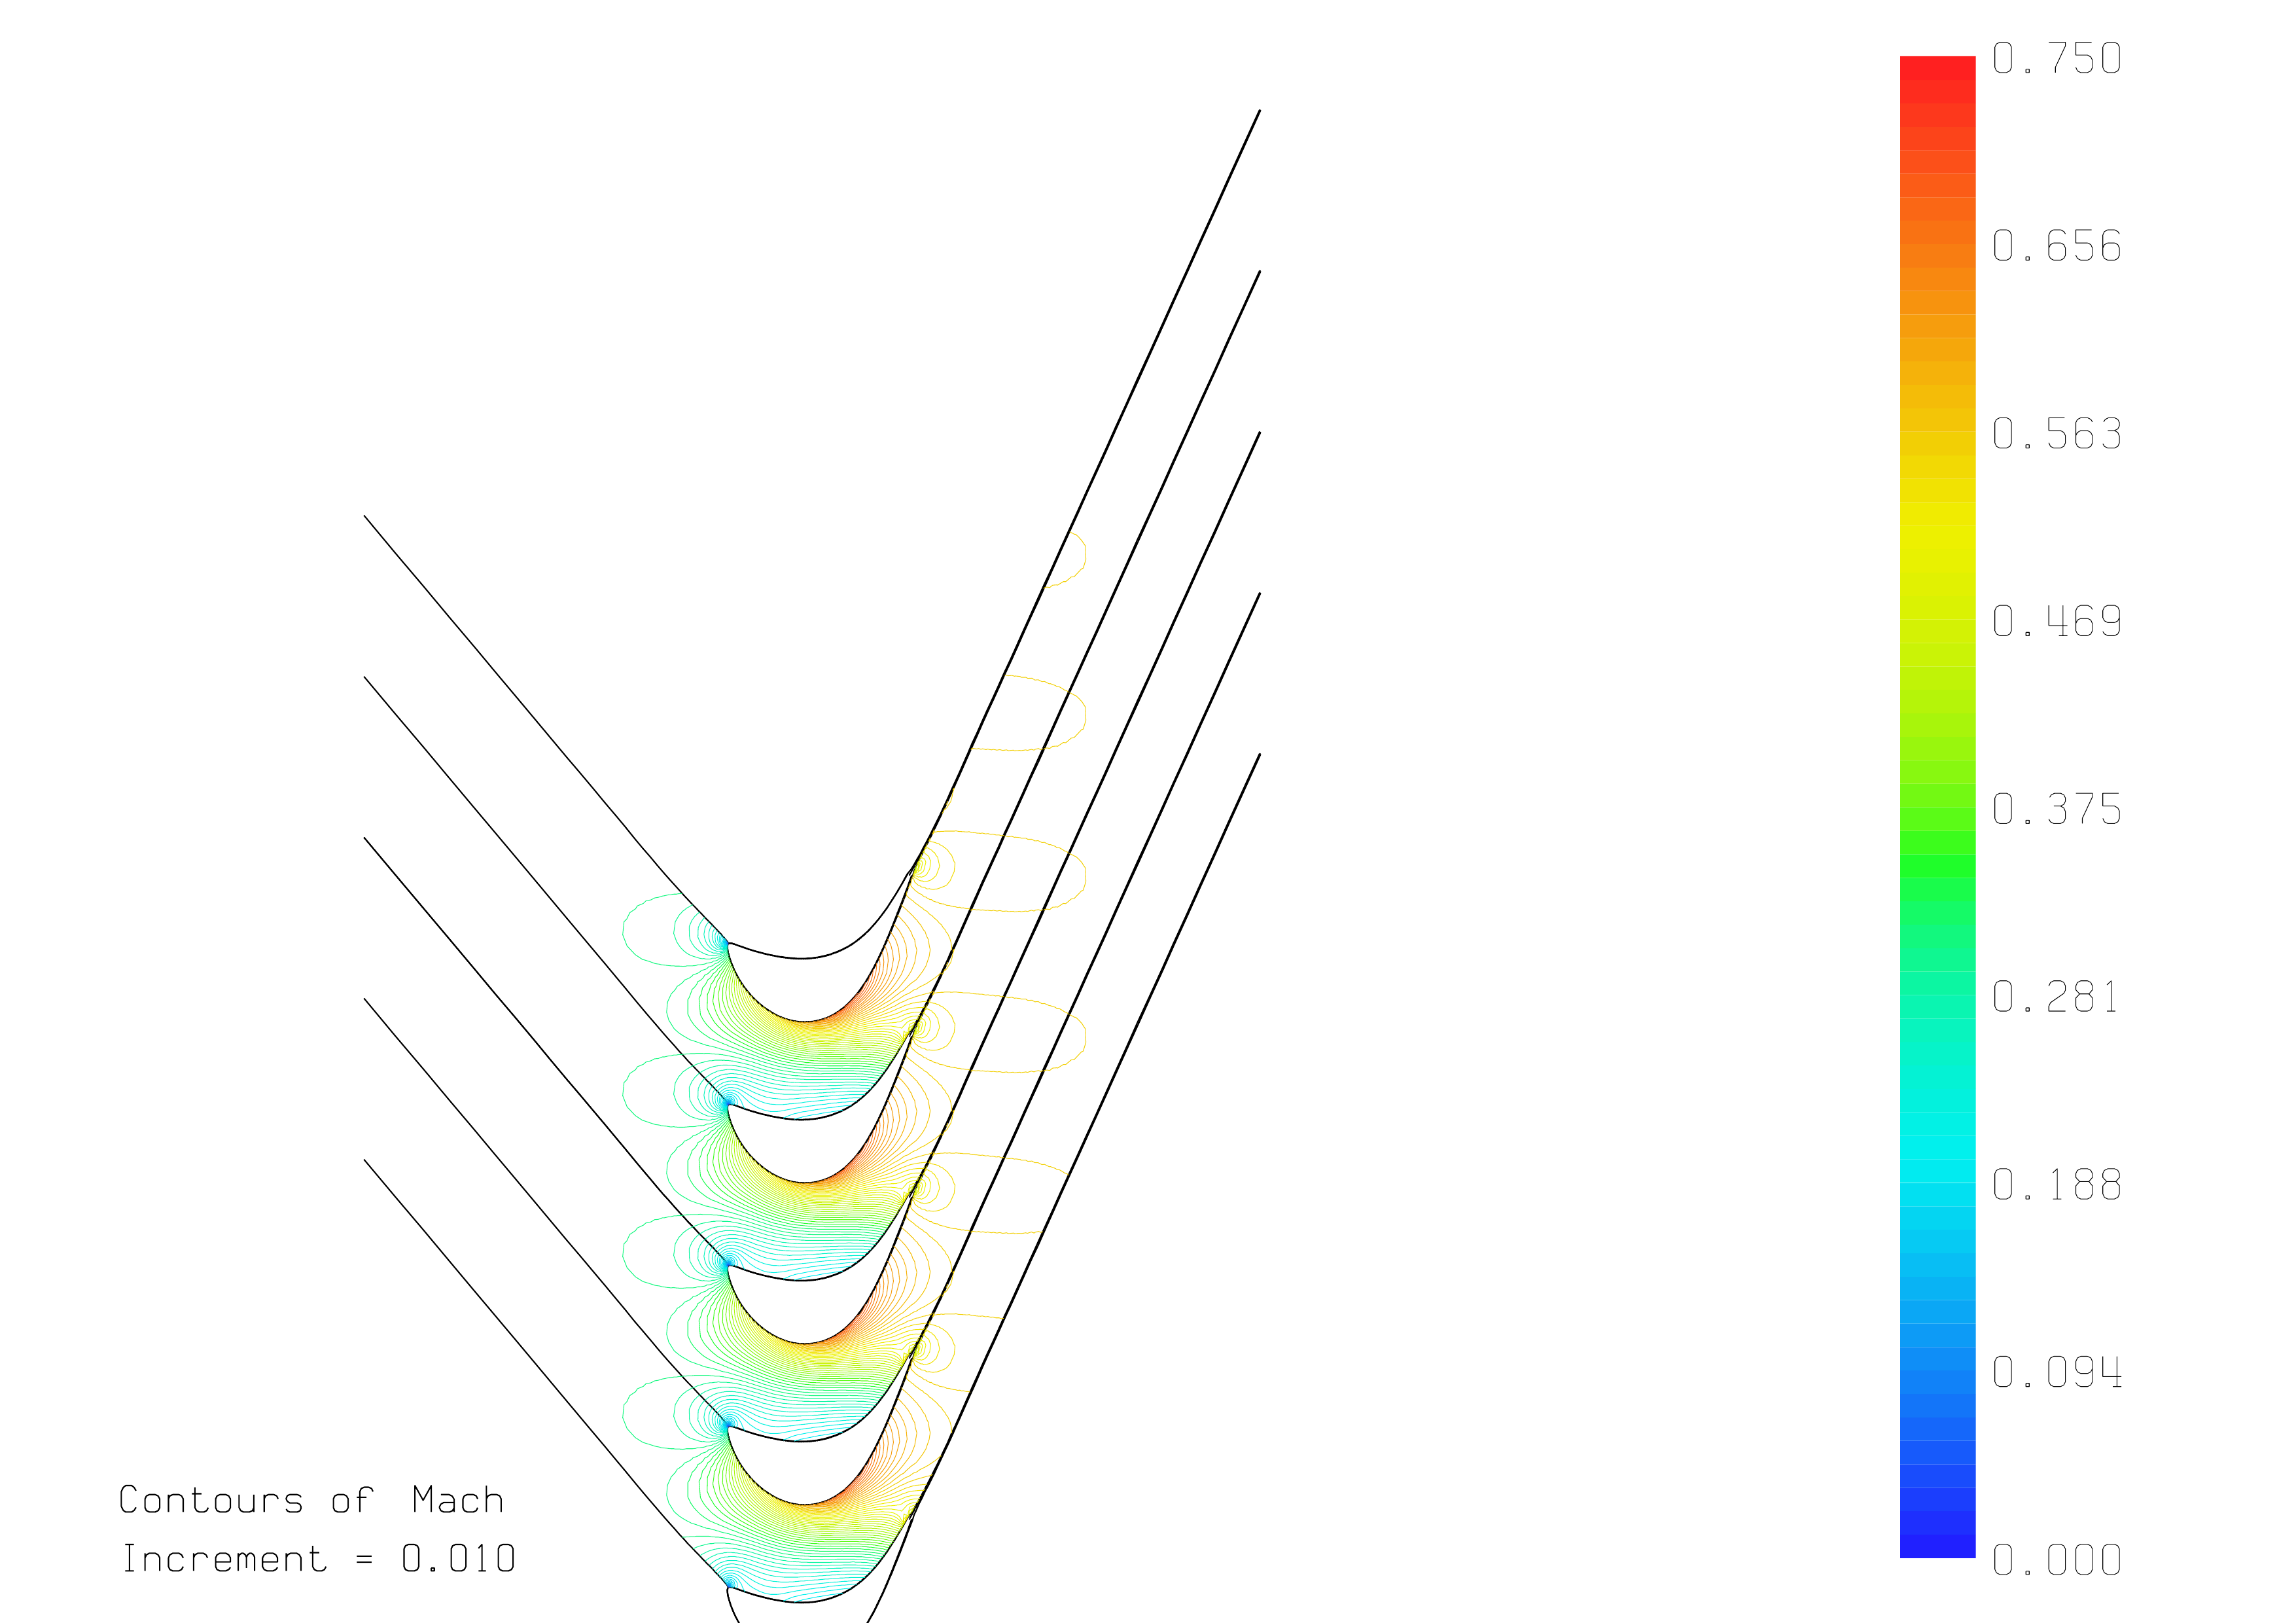
\includegraphics[scale=0.4]{./images/datablade120-4.png}
        \end{figure}
    \end{columns}
\end{frame}

% \begin{frame}{\texttt{MISES} Input -- Setup}
%     \begin{block}{Inputs}
%         \begin{itemize}
%         \item Flow properties:
%         \begin{itemize}
%             \item \texttt{MOUT = } $ M_2$: mixed outlet Mach flow
%             \item \texttt{SINL = } $\tan(\alpha_{1})$: inlet flow angle slope
%         \end{itemize}
%         \item Grid properties:
%         \begin{itemize}     
%             \item \texttt{F F}: grid setup, \texttt{H-type} grid for the inlet, the blade-to-blade plane and the outlet of the mesh
%         \end{itemize}
%         \item Turbulence:
%         \begin{itemize}
%             \item \texttt{REYin = } $Re = 6 \cdot 10^5$: flow Reynolds number
%             \item \texttt{NCRIT = } $n_{crit} = 4$: turbulence model parameter following Abu-Ghannam-Shaw model
%             \item \texttt{XTR1 = XTR2 = } $0.15$: imposed turbulence transition point over the blade
%         \end{itemize}
%     \end{itemize}
%     \end{block}
% \end{frame}

% \begin{frame}{\texttt{MISES} Input -- Properties}
%     \begin{alertblock}{Grid properties and test}
%         After many tests comparing \texttt{H-type} grid with \texttt{I-type} grid. The \texttt{H-type} grid allows faster execution time for the flow computation with neglecting difference on the flow output to \texttt{I-type} based simulations. This because shock waves are not present inside the domain.
%     \end{alertblock}
%     \begin{alertblock}{Turbulence properties}
%         \begin{itemize}
%             \item The $n_{crit}$ parameter has been chosen looking at a \texttt{MISES} input file for a turbine blade that sits in the working range conditions.
%             \item During the simulation, the turbulence model will then adapt the transition points to the most physical positions on the blade. This number is setup for reducing simulation convergence steps.
%         \end{itemize}
%     \end{alertblock}
% \end{frame}

% \begin{frame}{\texttt{MISES} simulation}
%     \begin{block}{Simulation}
%         \begin{itemize}
%             \item \texttt{ISMOM = 4}: this is the setup to attack the problem. The flow is studied as isentropic in the whole system except where shocks are present (which in this range of study are not so common). The switch from one solver to another is dictate by the $\rho$ field.
%             \item Log files are generated after each simulation for convergence tracking and flow properties study.
%             \item Computation of the Mach distribution over the blade.
%         \end{itemize}
%     \end{block}
% \end{frame}

% \hidelogo
% \begin{frame}{Postprocessing}
%     \begin{alertblock}{Load error computation}
%         The steps followed for the error computation on the aerodynamic load are:
%         \begin{itemize}
%             \item \texttt{MISES} computation
%             \item \texttt{MISES} call that generated Mach distribution over the blade
%             \item Reading of the Mach distribution file getting Mach curve and $M_{TE}$ for the Mach fraction generation
%             \item Computation of the RMSE error using the aerodynamic style target and the Mach fraction load converted in surface fraction. 
%             \item Cost computation 
%         \end{itemize}
%     \end{alertblock}
% \end{frame}
% \begin{frame}{Cost Function}
%     The cost function for the optimization of the blade is:
%     \begin{align*}
%         \Delta \alpha_2 & = | \alpha_{2, \texttt{MISES}} - \alpha_2 | \\ 
%         cost            & = RMSE \cdot \big[1 + 0.01 \cdot \big( 2 \cdot max(0, \Delta \alpha_{2} - \alpha_{th}) \big)^2 \big] \notag
%     \end{align*}
%     \begin{itemize}
%         \item The cost function allows to reduce the outlet flow angle error and the error on the load distribution at the same time. 
%         \item $\Delta \alpha_2$ is the absolute value of the error over the exit flow angle.
%         \item The $\alpha_{th}$ value is a threshold on the outlet flow error.
%     \end{itemize}
% \end{frame}


% \chapter{\texttt{datablade}}
\label{chapter:code}

This chapter introduces the \textbf{code} developed for the \textbf{database generation} and \textbf{analysis}. 
It will also explain the main aspects of the \textbf{code} in terms of \textbf{blade generation} and \textbf{optimization strategy}.
The code has been named \texttt{datablade}.

\section{Structure}

Figure~\ref{fig:databladeStructure} represents the directory subdivision of \texttt{datablade}. 
The program structure is based on blocks that can be combined for different purposes.  

\begin{figure}[!h]
  \tikzstyle{every node}=[draw=black,thick,anchor=west]
  \tikzstyle{selected}=[draw=red,fill=red!30]
  \tikzstyle{optional}=[dashed,fill=gray!50]
  \tikzstyle{plain}=[draw=none,anchor=west]
  \begin{minipage}{0.5\textwidth}
    \centering
    \begin{tikzpicture}[
      grow via three points={one child at (0.5,-0.7) and
      two children at (0.5,-0.7) and (0.5,-1.4)},
      edge from parent path={(\tikzparentnode.south) |- (\tikzchildnode.west)},
      scale=1]
      \texttt{
      \node {datablade}
        child { node {docs}}		
        child { node {misc}}
        child { node {module}}
        child { node [selected] {src}}
        child { node {test}}
        child { node [plain] {LICENSE}}
        child { node [plain] {setup.py}}
        child { node [plain] {setup.cfg}}
        child { node [plain] {README.md}};
      }
    \end{tikzpicture}
  \end{minipage}
  \begin{minipage}{0.5\textwidth}
    \centering
    \begin{tikzpicture}[
      font=\scriptsize,
      grow via three points={one child at (0.5,-0.7) and
      two children at (0.5,-0.7) and (0.5,-1.4)},
      edge from parent path={(\tikzparentnode.south) |- (\tikzchildnode.west)},
      scale=1]
      \texttt{
      \node [selected] {datablade/src}
        child { node {compileLIB}}
        child { node {databaseLIB}}
        child { node {execLIB}}
        child { node {kulfanLIB}}
        child { node {loadLIB}}
        child { node {misesLIB}}
        child { node {optimizationLIB}}
        child { node {performanceLIB}}
        child { node {postProcessingLIB}};
      }
    \end{tikzpicture}
  \end{minipage}
  \caption{\texttt{datablade} structure}
  \label{fig:databladeStructure}
\end{figure}

\section{Configuration File}

\texttt{datablade} optimization is configured using a \textbf{configuration file}. The configuration file is in \texttt{.json} format for allowing better \textbf{reading} and \textbf{handability}.

The following listings are parts of the configuration file - \texttt{config.json} - used in  \texttt{datablade}. All the dictionary entries are called \textit{as closer as possible} to the physical variables.

Listing~\ref{listing:configGuess} initilizes the initial guess for the blade optimization. Starting from its geometry - camberline, suction side and pressure side properties - and 
allocating the pitch and the trailing edge radius (which is kept constant at $R_{TE} = 1.25 \cdot 10^{-2}$ for the whole database).

\lstinputlisting[language=json, firstline=2, lastline=30, caption=\texttt{config.json} structure: initial guess ($\boldsymbol{x}_0$)., label=listing:configGuess]{./code/config.json.txt}

Listing~\ref{listing:configAero} defines the aerodynamic style and aerodynamic duty of the blade.

\lstinputlisting[language=json, firstline=31, lastline=44, caption=\texttt{config.json} structure: aerodynamic style and aerodynamic duty setup., label=listing:configAero]{./code/config.json.txt}

Listing~\ref{listing:configMises} sets the \texttt{MISES} simulation's entries and defines the parameters used in the cost function.

\lstinputlisting[language=json, firstline=57, lastline=72, caption=\texttt{config.json} structure: \texttt{MISES} configuration and cost function parameters., label=listing:configMises]{./code/config.json.txt}

At the end of \texttt{config.json}, in Listing~\ref{listing:configOpt}, there is the definition of the optimization strategy used in \texttt{datablade}.

\lstinputlisting[language=json, firstline=73, lastline=115, caption=\texttt{config.json} structure: optimization strategy setup., label=listing:configOpt]{./code/config.json.txt}

\section{Optimization}

The optimization algorithm used in \texttt{datablade} is a classic \textbf{gradient-free} method. 
The method used is the \textbf{Simplex} method~\cite{nelder1965simplex}. 
Even though the method finds the \textbf{local minima}, satisfactory results can be guaranteed using:

\begin{itemize}
    \item an appropriate choice of the initial guess, $\boldsymbol{x}_0$ 
    \item a \textbf{dimensionality adaptation strategy} for the problem
    \item an appropriate cost function which guarantees reliable results
\end{itemize}

\subsection{Dimensionality Adaptation}

% The blade optimization is a multi dimensional optimization problem which translates in a high cost in time and resources for 
% the computation of the optimum. Because of this problem, it is necessary to find a \textit{smart} way for the optimization of the blades. 
% The optimization strategy adapted in this work allows reaching good results for the generation of data that will be part of the database.
% This strategy consists in optimizing the blade varying the dimensionality of the problem. 

% The optimizer starts optimizing a blade parametrized with few parameters. 
% A low degree of freedom blade cannot generate a satisfactory result but, on the other hand, 
% it allows to flatten the design space avoiding \textit{bad design intervals} - in which normally the optimizer fails to converge.
% Once the low parameters optimization has converged, it is very likely that an increase in degree of freedom generates a better solution. 

% It has been tested that the best performance are reached doubling the degree of freedom of the blade parametrization after every optimization.

% If a blade converged with a low degree of freedom parametrization, the computed blade is scaled such that the database
% is populated by blade parametrized with the same number of parameters.

The optimization of blades poses a challenging multidimensional optimization problem, demanding significant time and resources to attain the optimal solution. Given this complexity, an \textit{intelligent approach} is necessary to streamline blade optimization. The strategy employed in this study demonstrates the ability to yield \textit{favorable outcomes} for constructing the database. This strategy involves optimizing blades by \textbf{manipulating the dimensionality of the problem}~\cite{clark2019step}.

The optimization process initiates by optimizing a blade with a \textbf{limited set of parameters}. While a blade with restricted degrees of freedom \textbf{may not produce an ideal outcome}, it does contribute to \textbf{flattening the design space}, thereby \textbf{mitigating unfavorable design intervals} where the optimizer might struggle to converge. Once optimization with fewer parameters achieves convergence, it's highly probable that increasing the degree of freedom will lead to \textbf{improved solutions}.

Empirical tests have revealed that the most favorable outcomes are achieved by \textbf{doubling} the degree of freedom in blade parametrization after each optimization cycle. Should a blade successfully converge with a low degree of freedom parametrization, the computed blade is subsequently scaled to populate the database with blades parametrized with the same number of parameters.

\subsection{Cost Function}

The blade optimization is related to two main errors: 

\begin{itemize}
    \item the \textbf{load error} over the blade, which is computed as the root mean squared error over the loading 
    \item the \textbf{flow exit angle error}
\end{itemize}

The root mean squared error is computed using Equation~(\ref{eqn:RMSE}).
The exit angle flow error is then computed using Equation~(\ref{eqn:angleError}). 

\begin{align}
    RMSE            & = \sqrt{\frac{1}{N_{points}} \cdot \sum_{i = 1}^{N_{points}} \Bigg( \frac{M_{real}}{M_{TE, real}} \Bigg|_{i} - \frac{M_{target}}{M_{TE, target}} \Bigg|_{i} \Bigg)^2} 
    \label{eqn:RMSE} \\ 
    \Delta \alpha_2 & = \Big| \alpha_{2, real} - \alpha_{2, target} \Big| 
    \label{eqn:angleError} 
\end{align}

Equation~(\ref{eqn:RMSE}) gets the Mach fraction distribution along the blade using 
the \texttt{.dat} file computed by \texttt{EDP} module in \texttt{MISES} and the Mach 
fraction distribution using the aerodynamic style curve computed in Chapter~\ref{chapter:framework}.

Once $RMSE$ and $\Delta \alpha_2$ have been computed, the cost function, Equation~(\ref{eqn:costFunction}), is a blend of those properties.
It is important that the cost function relates the $RMSE$ and $\Delta \alpha_2$ with a \textbf{product}; this in order
to reduce the \textit{competition} between the two variables during the optimization.

\begin{equation}
    cost = RMSE \cdot \Big[ 1 + 0.04 \cdot \Big( max \Big( 0, \ \Delta \alpha_2 - 1.0 \Big) \Big)^{2.0} \Big]
    \label{eqn:costFunction}
\end{equation}

Equation~\ref{eqn:costFunction} features the product between the $RMSE$ with another term which is a blend of different quantities.
The $0.04$ factor represents a scale which adapts the angle error to the overall cost function, it dictates how important the angle error, 
$\Delta \alpha_2$, should be compared to the $RMSE$. The scaling value acts on the terms in round parenteses. 
The value in the round parenteses is a threshold switch for the angle error. The threshold is set up by the 
$max(0, \ \Delta \alpha_2 - 1.0 )$ term. Once $ \Delta \alpha_2 - 1.0 > 0$, the switch activates and $\Delta \alpha_2$ contributes to the cost function.
On top of that, the \textit{switch} is \textbf{squared}; this in order to allow a \textbf{smooth transition of the error} from a region where \textit{just}
$RMSE$ contributes to the cost function - for $ \Delta \alpha_2 - 1.0 \leq 0$ - to the region where both $RMSE$ and $\Delta \alpha_2$ contribute to the overall cost function
- for $ \Delta \alpha_2 - 1.0 > 0$.

% The cost function has a double purpose. On one hand it generates a \textit{law} which 
% defines the convergence properties of the optimization algorithm. On the other hand 
% it provides a \textit{threshold of acceptability} for the optimized blades. If the value
% of the cost function for an optimized blade is high, this blade can be not taken into account 
% in order to have a more accurate database.

The cost function serves a dual purpose. Firstly, it establishes a \textit{guideline} governing the convergence behavior of 
the optimization algorithm. Secondly, it provides a \textit{threshold of acceptability} for the optimized blades. 
If the cost function value for an optimized blade is high, that particular blade might be excluded to ensure a more precise database.

\section{Optimizer}

On top of the optimization strategy there is the optimizer. 
The \texttt{datablade} optimizer combines the \texttt{MISES} software with the \texttt{scipy} module~\cite{2020SciPy-NMeth}.
These two components allow good performance and robustness. 

Figure~\ref{alg:datablade} illustrates how the blade is optimized by \texttt{datablade}.
It comprehends the optimization algorithm keeping the blade dimensionality fixed alongside 
the scaling process to increase convergence. Figure~\ref{alg:datablade} starts with the loading 
of the configuration file, \texttt{config.json}, which provides the initial guess - where the 
optimization starts -, the aerodynamic style and the aerodynamic duty of the blade. Once 
these properties are loaded, the program starts to optimize the blade using an
optimization based on the dimensionality adaptation of the blade to the problem. 


\begin{figure}[!h]

    \centering
    
    \resizebox{\textwidth}{!}{
    \begin{tikzpicture}[
        font=\fontsize{9}{9}\ttfamily, 
        thick, 
        align=center, 
        node distance=0.45cm, 
        remember picture, 
        x=\textwidth, 
        y=\textheight,
        every node/.style={
            align=center,
            scale=1
        }
    ]
            
    % Start block
    \node[draw,
        rectangle,
        rounded corners,
        % minimum width=2.5cm,
        % minimum height=0.2cm
        ] (start) {START};
    
    % getting guess of the solution 
    \node[draw,
        trapezium, 
        trapezium stretches=true, % A later addition
        trapezium left angle=70, 
        trapezium right angle=110, 
        text centered,
        below=of start,      
        % minimum width=3.0cm,  
        % minimum height=1cm,
    ] (aerodynamicDuty) {aerodynamic duty setup\\$\alpha_1$, $\alpha_2$, $M_2$ and $Re$};  

    % getting guess of the solution 
    \node[draw,
        trapezium, 
        trapezium stretches=true, % A later addition
        trapezium left angle=70, 
        trapezium right angle=110, 
        text centered,
        below=of aerodynamicDuty,      
        % minimum width=3.0cm,  
        % minimum height=1cm,
     ] (aerodynamicStyle) {aerodynamic style setup\\$\frac{M_P}{M_{TE}}$, $\frac{L_P}{L_{surf}}$, $\frac{M_{LE}}{M_{TE}}\frac{M_2}{M_1}$ and $\frac{M_{PS}}{M_{TE}}\frac{M_2}{M_{1, ax}}$}; 

    % getting guess of the solution 
    \node[draw,
        trapezium, 
        trapezium stretches=true, % A later addition
        trapezium left angle=70, 
        trapezium right angle=110, 
        text centered, 
        below=of aerodynamicStyle,      
        % minimum width=3.0cm,  
        % minimum height=1cm,
    ] (guess) {guessing $\boldsymbol{x}_{0}$\\from \texttt{config.json}};  

    % dimensionality check
    \node[draw, 
        diamond,
        below=of guess
      ] (dimCheck) {$N_{suct} \leq N_{suct_{target}}$\\[0.1cm]$N_{press} \leq N_{press_{target}}$};
    
    % setting up control point
    \coordinate[right=6cm of dimCheck] (controlPoint) {};

    % convergence check
    \node[draw, 
        diamond,
        above=3cm of controlPoint
    ] (convCheck) {$iter > iterTol$\\[0.1cm]$cost < costTol$\\[0.1cm]$\sigma < \sigma_{tol}$};

    % x optimization
    \node[draw, 
        below=0.5cm of convCheck,
        % minimum width=6.5cm,  
        % minimum height=1cm,
    ] (xUpdate) {$\boldsymbol{x}$ update};
  
    % coordinate computation
    \node[draw, 
        below=of xUpdate,
        % minimum width=6.5cm,  
        % minimum height=1cm,
    ] (settingPar) {blade coordinates computation using\\ Kulfan parametrization};
    
    % ISET input file generation
    \node[draw,
        below=of settingPar,
        % minimum width=5.5cm,
        % minimum height=1cm,
        ] (ISETsetup) {setting up \texttt{ISET} configuration file};
    
    % ISES input file generation
    \node[draw,
        below=of ISETsetup,
        % minimum width=5.5cm,
        % minimum height=1cm,
    ] (ISESsetup) {setting up \texttt{ISES} configuration file};

    % ISET input file generation
    \node[draw,
        below=of ISESsetup,
        % minimum width=5.5cm,
        % minimum height=1cm,
    ] (MISEScomputation) {running \texttt{MISES} solver: grid generator, \\flow solver \& flow post-processing};
        
    % cost computation
    \node[draw,
        below=of MISEScomputation,
        % minimum width=5.5cm,
        % minimum height=1cm,
    ] (costComputation) {computing cost function};

    % end 
    \node[draw,
        rectangle,
        rounded corners,
        left=1cm of dimCheck,
    ] (end) {END};

    % coordinates for arrotw
    \coordinate[left=1.7cm of convCheck] (c1) {};
    \coordinate[] (c2) at (c1 |- costComputation) {};
    \coordinate[right=1.5cm of convCheck] (c3) {};
    \coordinate[below=0.35cm of convCheck] (c4) {};
    \coordinate[right=2cm of dimCheck] (c5) {};
    \coordinate[] (c6) at (c5 |- convCheck.north) {};
    \coordinate[right=1.7cm of convCheck] (c7) {};
    \coordinate[below=0.35cm of costComputation] (c8) {};
    \coordinate[] (c9) at (c7 |- c8) {};
    \coordinate[] (c10) at (dimCheck |- c9) {};
    \coordinate[left=0.5cm of dimCheck] (c11) {};

    % arrow drawing
    \draw[-latex] (start) to (aerodynamicDuty);
    \draw[-latex] (aerodynamicDuty) to (aerodynamicStyle);
    \draw[-latex] (aerodynamicStyle) to (guess);
    \draw[-latex] (guess) to (dimCheck);
    \draw[-latex] (dimCheck.east) -- node[anchor=south] {yes} (c5) -- (c6) to (convCheck.north);
    \draw[-latex] (convCheck.south) -- node[anchor=east] {no} (c4) to (xUpdate.north);
    \draw[-latex] (xUpdate) to (settingPar);
    \draw[-latex] (settingPar) to (ISETsetup);
    \draw[-latex] (ISETsetup) to (ISESsetup);
    \draw[-latex] (ISESsetup) to (MISEScomputation);
    \draw[-latex] (MISEScomputation) to (costComputation);
    \draw[-latex] (costComputation.west) -- (c2) -- (c1) to (convCheck.west);
    \draw[-latex] (convCheck.east) -- node[anchor=north] {yes} (c3) -- (c7) -- (c9) -- (c10) -- (dimCheck.south); 
    \draw[-latex] (dimCheck.west) -- node[anchor=south] {no} (c11) -- (end.east);

    \end{tikzpicture}
    }
    
    \caption{\texttt{datablade} optimizer structure.}
    \label{alg:datablade}
    
\end{figure}


% \begin{frame}{Database generation strategy}
    \newcommand\WIDTH{3.5cm}
    \newcommand\HEIGHT{1.5cm}
    \newcommand\Ydist{2cm}
    \newcommand\XPOS{4cm}
    \newcommand\TOTheight{5cm}
    \newcommand\TOTwidth{6cm}
    \newcommand\PTS{2pt}
    \newcommand\xSpace{0.5cm}

    \only<1>{
        \begin{figure}
            \centering
            \vspace*{0.5cm}
            \hspace*{0.3cm}
            \begin{tikzpicture}
    
    \node[draw,
        rectangle,
        text centered,
        line width = \PTS,
        minimum height = \TOTheight,
        minimum width = \TOTwidth
    ] (optimizationProcess) at (0, 0) {\large{\textbf{Optimization}}};

    % \node[
    %     below right = 0.5cm and 0.5cm of optimizationProcess.north west 
    % ] {
    %     
\includegraphics[scale=0.08]{./MITlogo.png}
    % };

    % \node[
    %     above left = 0.15cm and 0.5cm of optimizationProcess.south east 
    % ] {
    %     
\includegraphics[scale=0.3]{./SCIPYlogo.png}
    % };

    \node[draw,
        rectangle,
        text centered,
        line width = \PTS,
        % minimum width = \WIDTH,
        minimum height = \HEIGHT,
        right = 2*\xSpace of optimizationProcess
    ] (database) {\large{\textbf{Database}}};
    
    \coordinate[left=\xSpace of optimizationProcess.west]  (c1) {};
    \coordinate[above=\Ydist of c1]                      (c2) {};
    \coordinate[below=\Ydist of c1]                      (c3) {};

    \node[draw,
        rectangle,
        text centered,
        line width = \PTS,
        minimum width = \WIDTH,
        minimum height = \HEIGHT,
        left = \xSpace of c2
    ] (designSpace) {\large{\textbf{\makecell[c]{Design space\\reduction}}}};

    \node[draw,
        rectangle,
        text centered,
        line width = \PTS,
        minimum width = \WIDTH,
        minimum height = \HEIGHT,
        left = \xSpace of c1
    ] (constr) {\large{\textbf{Constraints}}};

    \node[draw,
        rectangle,
        text centered,
        line width = \PTS,
        minimum width = \WIDTH,
        minimum height = \HEIGHT,
        left = \xSpace of c3
    ] (obj) {\large{\textbf{Objectives}}};

    \draw[-latex, line width = 1pt] (designSpace) -- (c2) -- (c1) to (optimizationProcess.west);
    \draw[-latex, line width = 1pt] (constr) to (optimizationProcess.west);
    \draw[-latex, line width = 1pt] (obj) -- (c3) -- (c1) to (optimizationProcess.west);
    \draw[-latex, line width = 1pt] (optimizationProcess.east) to (database.west);

\end{tikzpicture}
            % 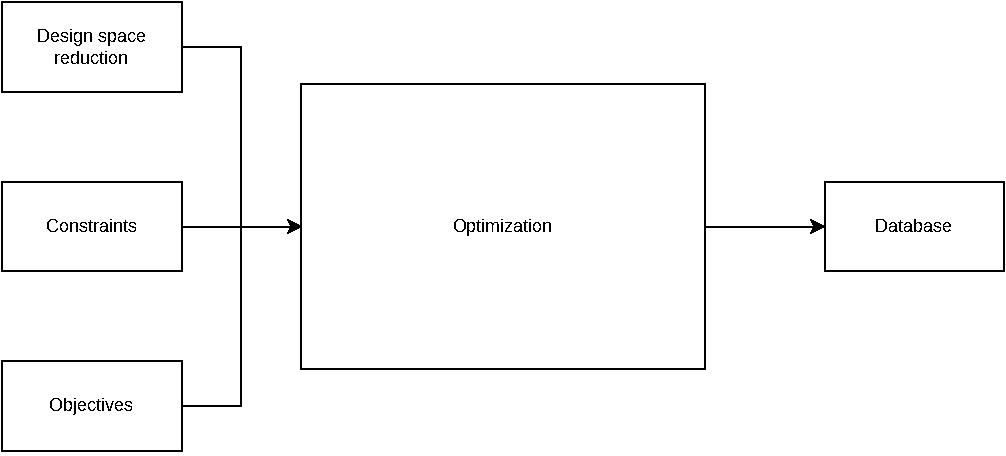
\includegraphics[page=1, scale=0.7]{pdf/databaseScheme-start.drawio}
        \end{figure}
    }
    \only<2>{
        \begin{figure}
            \centering
            \vspace*{0.5cm}
            \hspace*{0.3cm}
            \begin{tikzpicture}
    
    \node[draw,
        rectangle,
        text centered,
        line width = \PTS,
        minimum height = \TOTheight,
        minimum width = \TOTwidth
    ] (optimizationProcess) at (0, 0) {\large{\textbf{Optimization}}};

    % \node[
    %     below right = 0.5cm and 0.5cm of optimizationProcess.north west 
    % ] {
    %     
\includegraphics[scale=0.08]{./MITlogo.png}
    % };

    % \node[
    %     above left = 0.15cm and 0.5cm of optimizationProcess.south east 
    % ] {
    %     
\includegraphics[scale=0.3]{./SCIPYlogo.png}
    % };

    \node[draw,
        rectangle,
        text centered,
        line width = \PTS,
        % minimum width = \WIDTH,
        minimum height = \HEIGHT,
        right = 2*\xSpace of optimizationProcess
    ] (database) {\large{\textbf{Database}}};
    
    \coordinate[left=\xSpace of optimizationProcess.west]  (c1) {};
    \coordinate[above=\Ydist of c1]                      (c2) {};
    \coordinate[below=\Ydist of c1]                      (c3) {};

    \node[draw,
        rectangle,
        text centered,
        line width = \PTS,
        minimum width = \WIDTH,
        minimum height = \HEIGHT,
        left = \xSpace of c2
    ] (designSpace) {\large{\textbf{\makecell[c]{Kulfan\\parametrization}}}};

    \node[draw,
        rectangle,
        text centered,
        line width = \PTS,
        minimum width = \WIDTH,
        minimum height = \HEIGHT,
        left = \xSpace of c1
    ] (constr) {\large{\textbf{Constraints}}};

    \node[draw,
        rectangle,
        text centered,
        line width = \PTS,
        minimum width = \WIDTH,
        minimum height = \HEIGHT,
        left = \xSpace of c3
    ] (obj) {\large{\textbf{Objectives}}};

    \draw[-latex, line width = 1pt] (designSpace) -- (c2) -- (c1) to (optimizationProcess.west);
    \draw[-latex, line width = 1pt] (constr) to (optimizationProcess.west);
    \draw[-latex, line width = 1pt] (obj) -- (c3) -- (c1) to (optimizationProcess.west);
    \draw[-latex, line width = 1pt] (optimizationProcess.east) to (database.west);

\end{tikzpicture}
            % 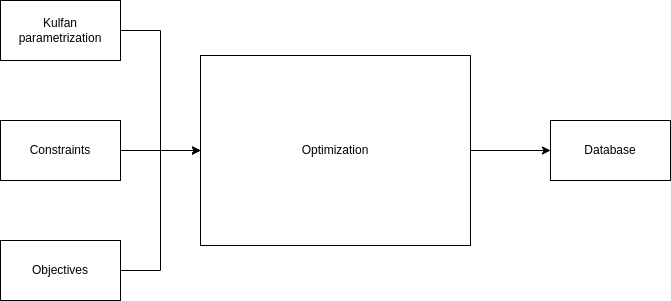
\includegraphics[page=1, scale=0.7]{pdf/databaseScheme-kulfan.drawio}
        \end{figure}
    }
    \only<3>{
        \begin{figure}
            \centering
            \vspace*{0.5cm}
            \hspace*{0.3cm}
            \begin{tikzpicture}
    
    \node[draw,
        rectangle,
        text centered,
        line width = \PTS,
        minimum height = \TOTheight,
        minimum width = \TOTwidth
    ] (optimizationProcess) at (0, 0) {\large{\textbf{Optimization}}};

    % \node[
    %     below right = 0.5cm and 0.5cm of optimizationProcess.north west 
    % ] {
    %     
\includegraphics[scale=0.08]{./MITlogo.png}
    % };

    % \node[
    %     above left = 0.15cm and 0.5cm of optimizationProcess.south east 
    % ] {
    %     
\includegraphics[scale=0.3]{./SCIPYlogo.png}
    % };

    \node[draw,
        rectangle,
        text centered,
        line width = \PTS,
        % minimum width = \WIDTH,
        minimum height = \HEIGHT,
        right = 2*\xSpace of optimizationProcess
    ] (database) {\large{\textbf{Database}}};
    
    \coordinate[left=\xSpace of optimizationProcess.west]  (c1) {};
    \coordinate[above=\Ydist of c1]                      (c2) {};
    \coordinate[below=\Ydist of c1]                      (c3) {};

    \node[draw,
        rectangle,
        text centered,
        line width = \PTS,
        minimum width = \WIDTH,
        minimum height = \HEIGHT,
        left = \xSpace of c2
    ] (designSpace) {\large{\textbf{\makecell[c]{Kulfan\\parametrization}}}};

    \node[draw,
        rectangle,
        text centered,
        line width = \PTS,
        minimum width = \WIDTH,
        minimum height = \HEIGHT,
        left = \xSpace of c1
    ] (constr) {\large{\textbf{\makecell[c]{Aerodynamic\\Duty}}}};

    \node[draw,
        rectangle,
        text centered,
        line width = \PTS,
        minimum width = \WIDTH,
        minimum height = \HEIGHT,
        left = \xSpace of c3
    ] (obj) {\large{\textbf{Objectives}}};

    \draw[-latex, line width = 1pt] (designSpace) -- (c2) -- (c1) to (optimizationProcess.west);
    \draw[-latex, line width = 1pt] (constr) to (optimizationProcess.west);
    \draw[-latex, line width = 1pt] (obj) -- (c3) -- (c1) to (optimizationProcess.west);
    \draw[-latex, line width = 1pt] (optimizationProcess.east) to (database.west);

\end{tikzpicture}
            % 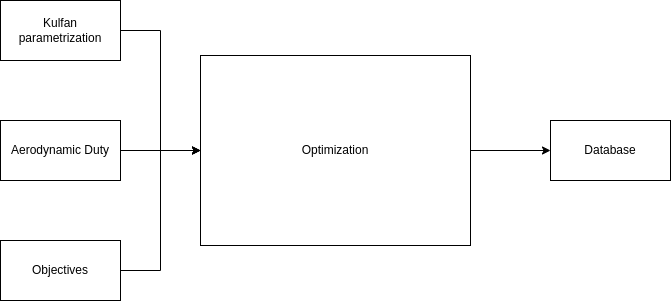
\includegraphics[page=1, scale=0.7]{pdf/databaseScheme-aerodynamicDuty.drawio}
        \end{figure}
    }
    \only<4>{
        \begin{figure}
            \centering
            \vspace*{0.5cm}
            \hspace*{0.3cm}
            \begin{tikzpicture}
    
    \node[draw,
        rectangle,
        text centered,
        line width = \PTS,
        minimum height = \TOTheight,
        minimum width = \TOTwidth
    ] (optimizationProcess) at (0, 0) {\large{\textbf{Optimization}}};

    % \node[
    %     below right = 0.5cm and 0.5cm of optimizationProcess.north west 
    % ] {
    %     
\includegraphics[scale=0.08]{./MITlogo.png}
    % };

    % \node[
    %     above left = 0.15cm and 0.5cm of optimizationProcess.south east 
    % ] {
    %     
\includegraphics[scale=0.3]{./SCIPYlogo.png}
    % };

    \node[draw,
        rectangle,
        text centered,
        line width = \PTS,
        % minimum width = \WIDTH,
        minimum height = \HEIGHT,
        right = 2*\xSpace of optimizationProcess
    ] (database) {\large{\textbf{Database}}};
    
    \coordinate[left=\xSpace of optimizationProcess.west]  (c1) {};
    \coordinate[above=\Ydist of c1]                      (c2) {};
    \coordinate[below=\Ydist of c1]                      (c3) {};

    \node[draw,
        rectangle,
        text centered,
        line width = \PTS,
        minimum width = \WIDTH,
        minimum height = \HEIGHT,
        left = \xSpace of c2
    ] (designSpace) {\large{\textbf{\makecell[c]{Kulfan\\parametrization}}}};

    \node[draw,
        rectangle,
        text centered,
        line width = \PTS,
        minimum width = \WIDTH,
        minimum height = \HEIGHT,
        left = \xSpace of c1
    ] (constr) {\large{\textbf{\makecell[c]{Aerodynamic\\Duty}}}};

    \node[draw,
        rectangle,
        text centered,
        line width = \PTS,
        minimum width = \WIDTH,
        minimum height = \HEIGHT,
        left = \xSpace of c3
    ] (obj) {\large{\textbf{\makecell[c]{Aerodynamic\\Style}}}};

    \draw[-latex, line width = 1pt] (designSpace) -- (c2) -- (c1) to (optimizationProcess.west);
    \draw[-latex, line width = 1pt] (constr) to (optimizationProcess.west);
    \draw[-latex, line width = 1pt] (obj) -- (c3) -- (c1) to (optimizationProcess.west);
    \draw[-latex, line width = 1pt] (optimizationProcess.east) to (database.west);

\end{tikzpicture}
            % 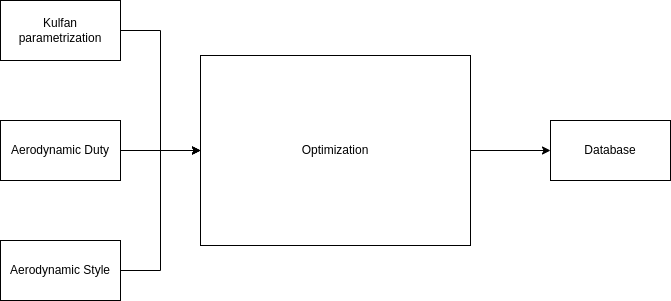
\includegraphics[page=1, scale=0.7]{pdf/databaseScheme-aerodynamicStyle.drawio}
        \end{figure}
    }
    \only<5>{
        \begin{figure}
            \centering
            \vspace*{0.5cm}
            \hspace*{0.3cm}
            \begin{tikzpicture}
    
    \node[draw,
        rectangle,
        text centered,
        line width = \PTS,
        minimum height = \TOTheight,
        minimum width = \TOTwidth
    ] (optimizationProcess) at (0, 0) {};

    \node[
        below right = 0.25cm and 0.25cm of optimizationProcess.north west 
    ] {
        
\includegraphics[scale=0.05]{./images/MITlogo.png}
    };

    \node[
        above left = 0.02cm and 0.02cm of optimizationProcess.south east 
    ] {
        
\includegraphics[scale=0.2]{./images/SCIPYlogo.png}
    };

    \node[draw,
        rectangle,
        text centered,
        line width = \PTS,
        % minimum width = 2cm,
        minimum height = \HEIGHT,
        right = 2*\xSpace of optimizationProcess
    ] (database) {\large{\textbf{Database}}};
    
    \coordinate[left=\xSpace of optimizationProcess.west]  (c1) {};
    \coordinate[above=\Ydist of c1]                      (c2) {};
    \coordinate[below=\Ydist of c1]                      (c3) {};

    \node[draw,
        rectangle,
        text centered,
        line width = \PTS,
        minimum width = \WIDTH,
        minimum height = \HEIGHT,
        left = \xSpace of c2
    ] (designSpace) {\large{\textbf{\makecell[c]{Kulfan\\parametrization}}}};

    \node[draw,
        rectangle,
        text centered,
        line width = \PTS,
        minimum width = \WIDTH,
        minimum height = \HEIGHT,
        left = \xSpace of c1
    ] (constr) {\large{\textbf{\makecell[c]{Aerodynamic\\Duty}}}};

    \node[draw,
        rectangle,
        text centered,
        line width = \PTS,
        minimum width = \WIDTH,
        minimum height = \HEIGHT,
        left = \xSpace of c3
    ] (obj) {\large{\textbf{\makecell[c]{Aerodynamic\\Style}}}};

    \draw[-latex, line width = 1pt] (designSpace) -- (c2) -- (c1) to (optimizationProcess.west);
    \draw[-latex, line width = 1pt] (constr) to (optimizationProcess.west);
    \draw[-latex, line width = 1pt] (obj) -- (c3) -- (c1) to (optimizationProcess.west);
    \draw[-latex, line width = 1pt] (optimizationProcess.east) to (database.west);

\end{tikzpicture}
            % 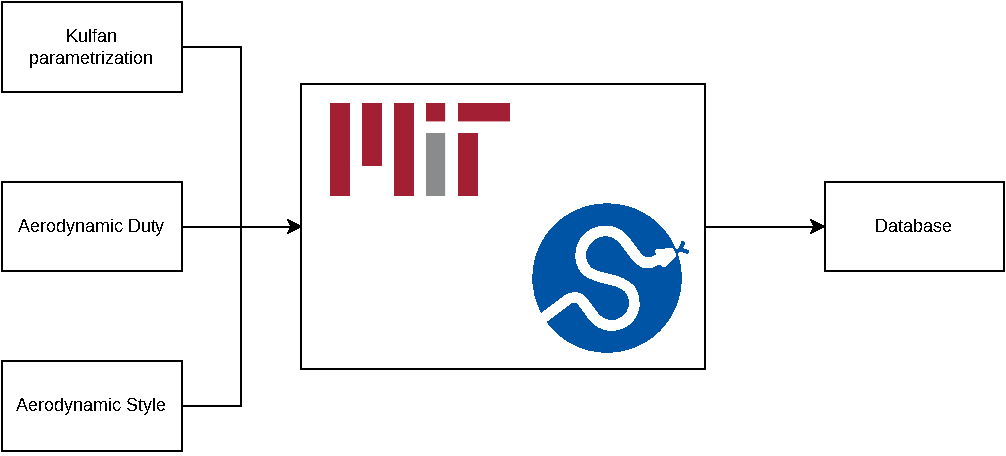
\includegraphics[page=1, scale=0.7]{pdf/databaseScheme-optimization.drawio}
        \end{figure}
    }
\end{frame}

\begin{frame}{Database points}
    \only<1>{
        \begin{columns}
            \column{0.5\textwidth}
            \begin{figure}
                \centering
                % \hspace*{-1cm}
                % \vspace{1cm}
                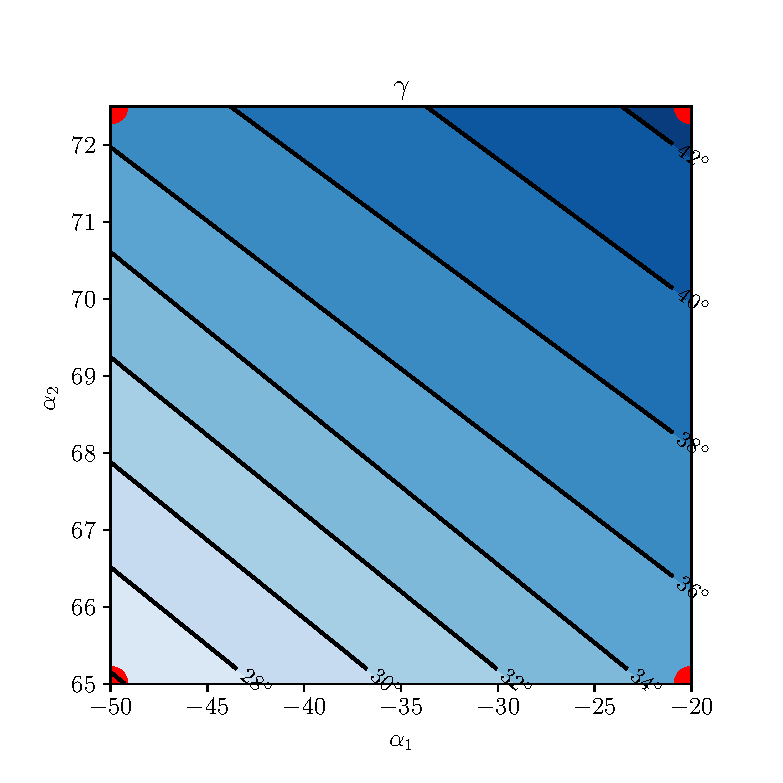
\includegraphics[scale=0.5]{images/staggerLinear.eps}
            \end{figure}
            \column{0.5\textwidth}
            \begin{itemize}
                \item Data optimization \textbf{starting from the boundaries of the domain} of study
                % \item From the \textbf{corner points} of the domain, it is \textbf{computed a new guess} for the optimization of the inner points
                % \item The new guess is made using a \textbf{linear interpolation} of optimized data 
                % \item Once this procedure generates \textbf{sufficient data for the ML training}, data collection is stopped
            \end{itemize}
        \end{columns}
    }
    \only<2>{
        \begin{columns}
            \column{0.5\textwidth}
            \begin{figure}
                \centering
                % \hspace*{-1cm}
                % \vspace{1cm}
                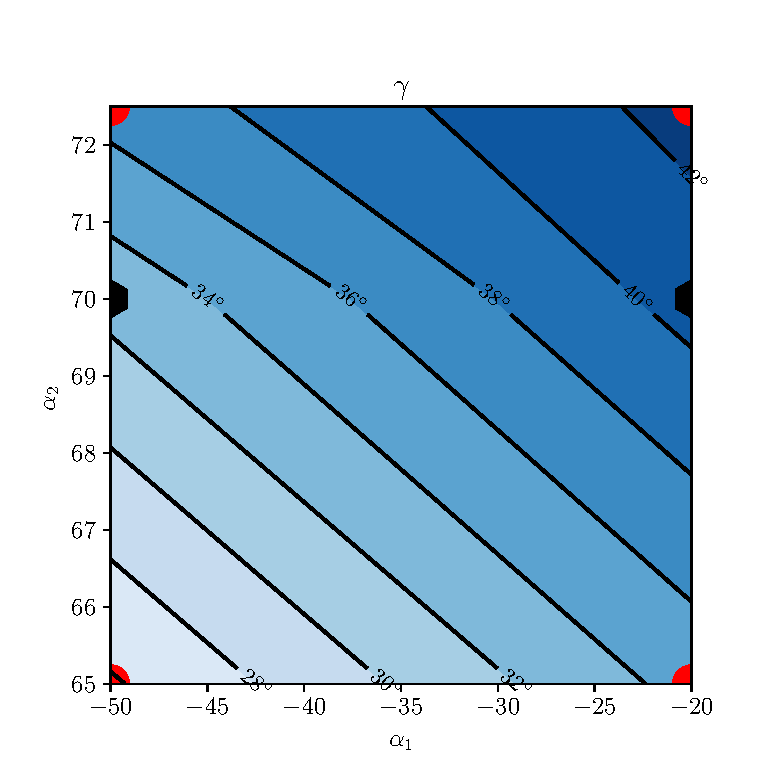
\includegraphics[scale=0.5]{images/staggerLinear1.eps}
            \end{figure}
            \column{0.5\textwidth}
            \begin{itemize}
                \item Data optimization \textbf{starting from the boundaries of the domain} of study
                \item From the \textbf{corner points} of the domain, it is \textbf{computed a new guess} for the optimization of the inner points
                \item The new guess is made using a \textbf{linear interpolation} of optimized data 
                % \item Once this procedure generates \textbf{sufficient data for the ML training}, data collection is stopped
            \end{itemize}
        \end{columns}
    }
    \only<3>{
        \begin{columns}
            \column{0.5\textwidth}
            \begin{figure}
                \centering
                % \hspace*{-1cm}
                % \vspace{1cm}
                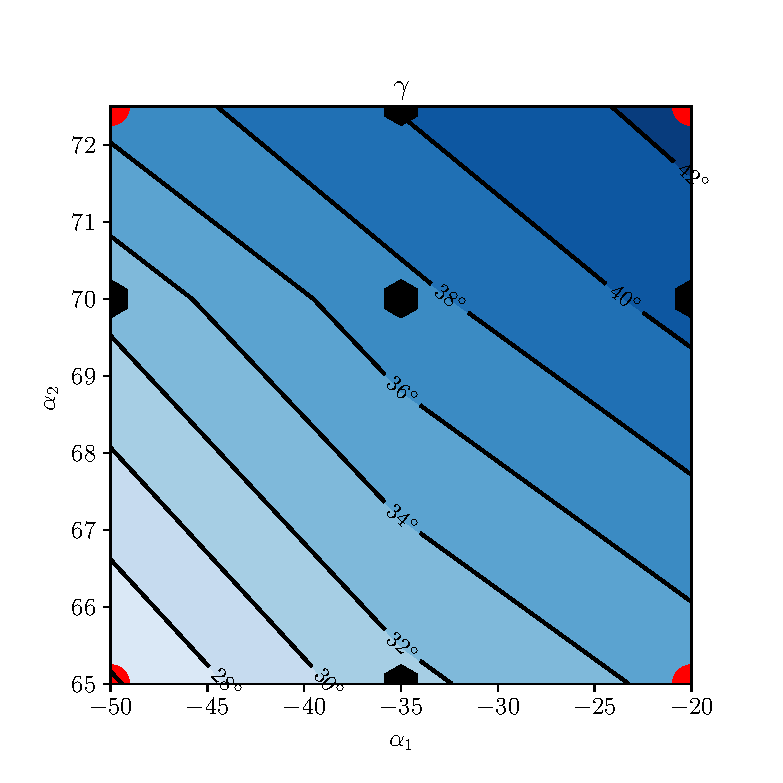
\includegraphics[scale=0.5]{images/staggerLinear2.eps}
            \end{figure}
            \column{0.5\textwidth}
            \begin{itemize}
                \item Data optimization \textbf{starting from the boundaries of the domain} of study
                \item From the \textbf{corner points} of the domain, it is \textbf{computed a new guess} for the optimization of the inner points
                \item The new guess is made using a \textbf{linear interpolation} of optimized data 
                % \item Once this procedure generates \textbf{sufficient data for the ML training}, data collection is stopped
            \end{itemize}
        \end{columns}
    }
    \only<4>{
        \begin{columns}
            \column{0.5\textwidth}
            \begin{figure}
                \centering
                % \hspace*{-1cm}
                % \vspace{1cm}
                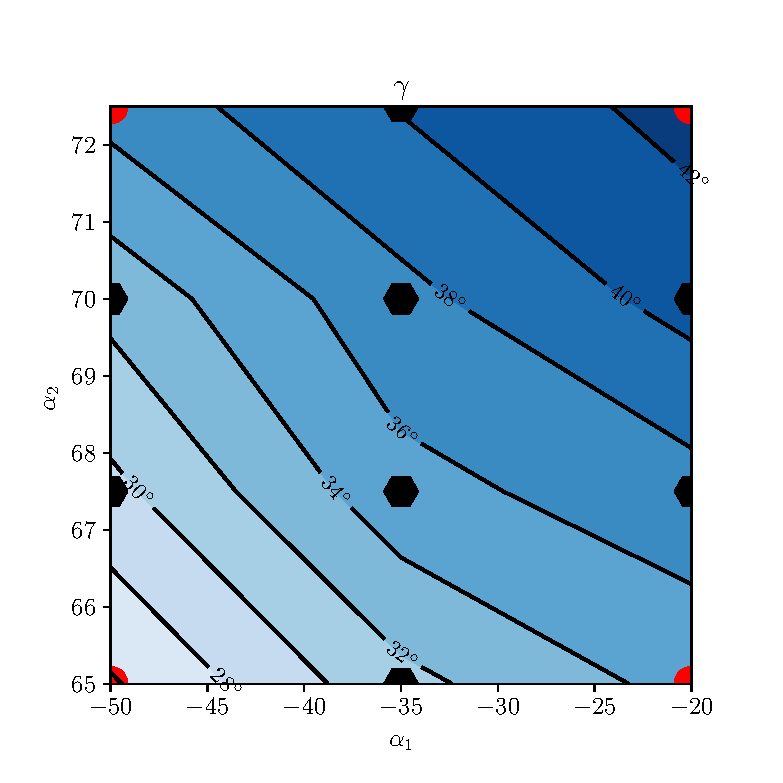
\includegraphics[scale=0.5]{images/staggerComplete.eps}
            \end{figure}
            \column{0.5\textwidth}
            \begin{itemize}
                \item Data optimization \textbf{starting from the boundaries of the domain} of study
                \item From the \textbf{corner points} of the domain, it is \textbf{computed a new guess} for the optimization of the inner points
                \item The new guess is made using a \textbf{linear interpolation} of optimized data 
                \item Once this procedure generates \textbf{sufficient data for the ML training}, data collection is stopped
            \end{itemize}
        \end{columns}
    }
\end{frame}

\begin{frame}{Inner points}
    The \textbf{new guess} on the blade shape for the inner points of the database is made by a \textbf{linear interpolation of the corner points} geometry.
    \begin{figure}
        \centering
        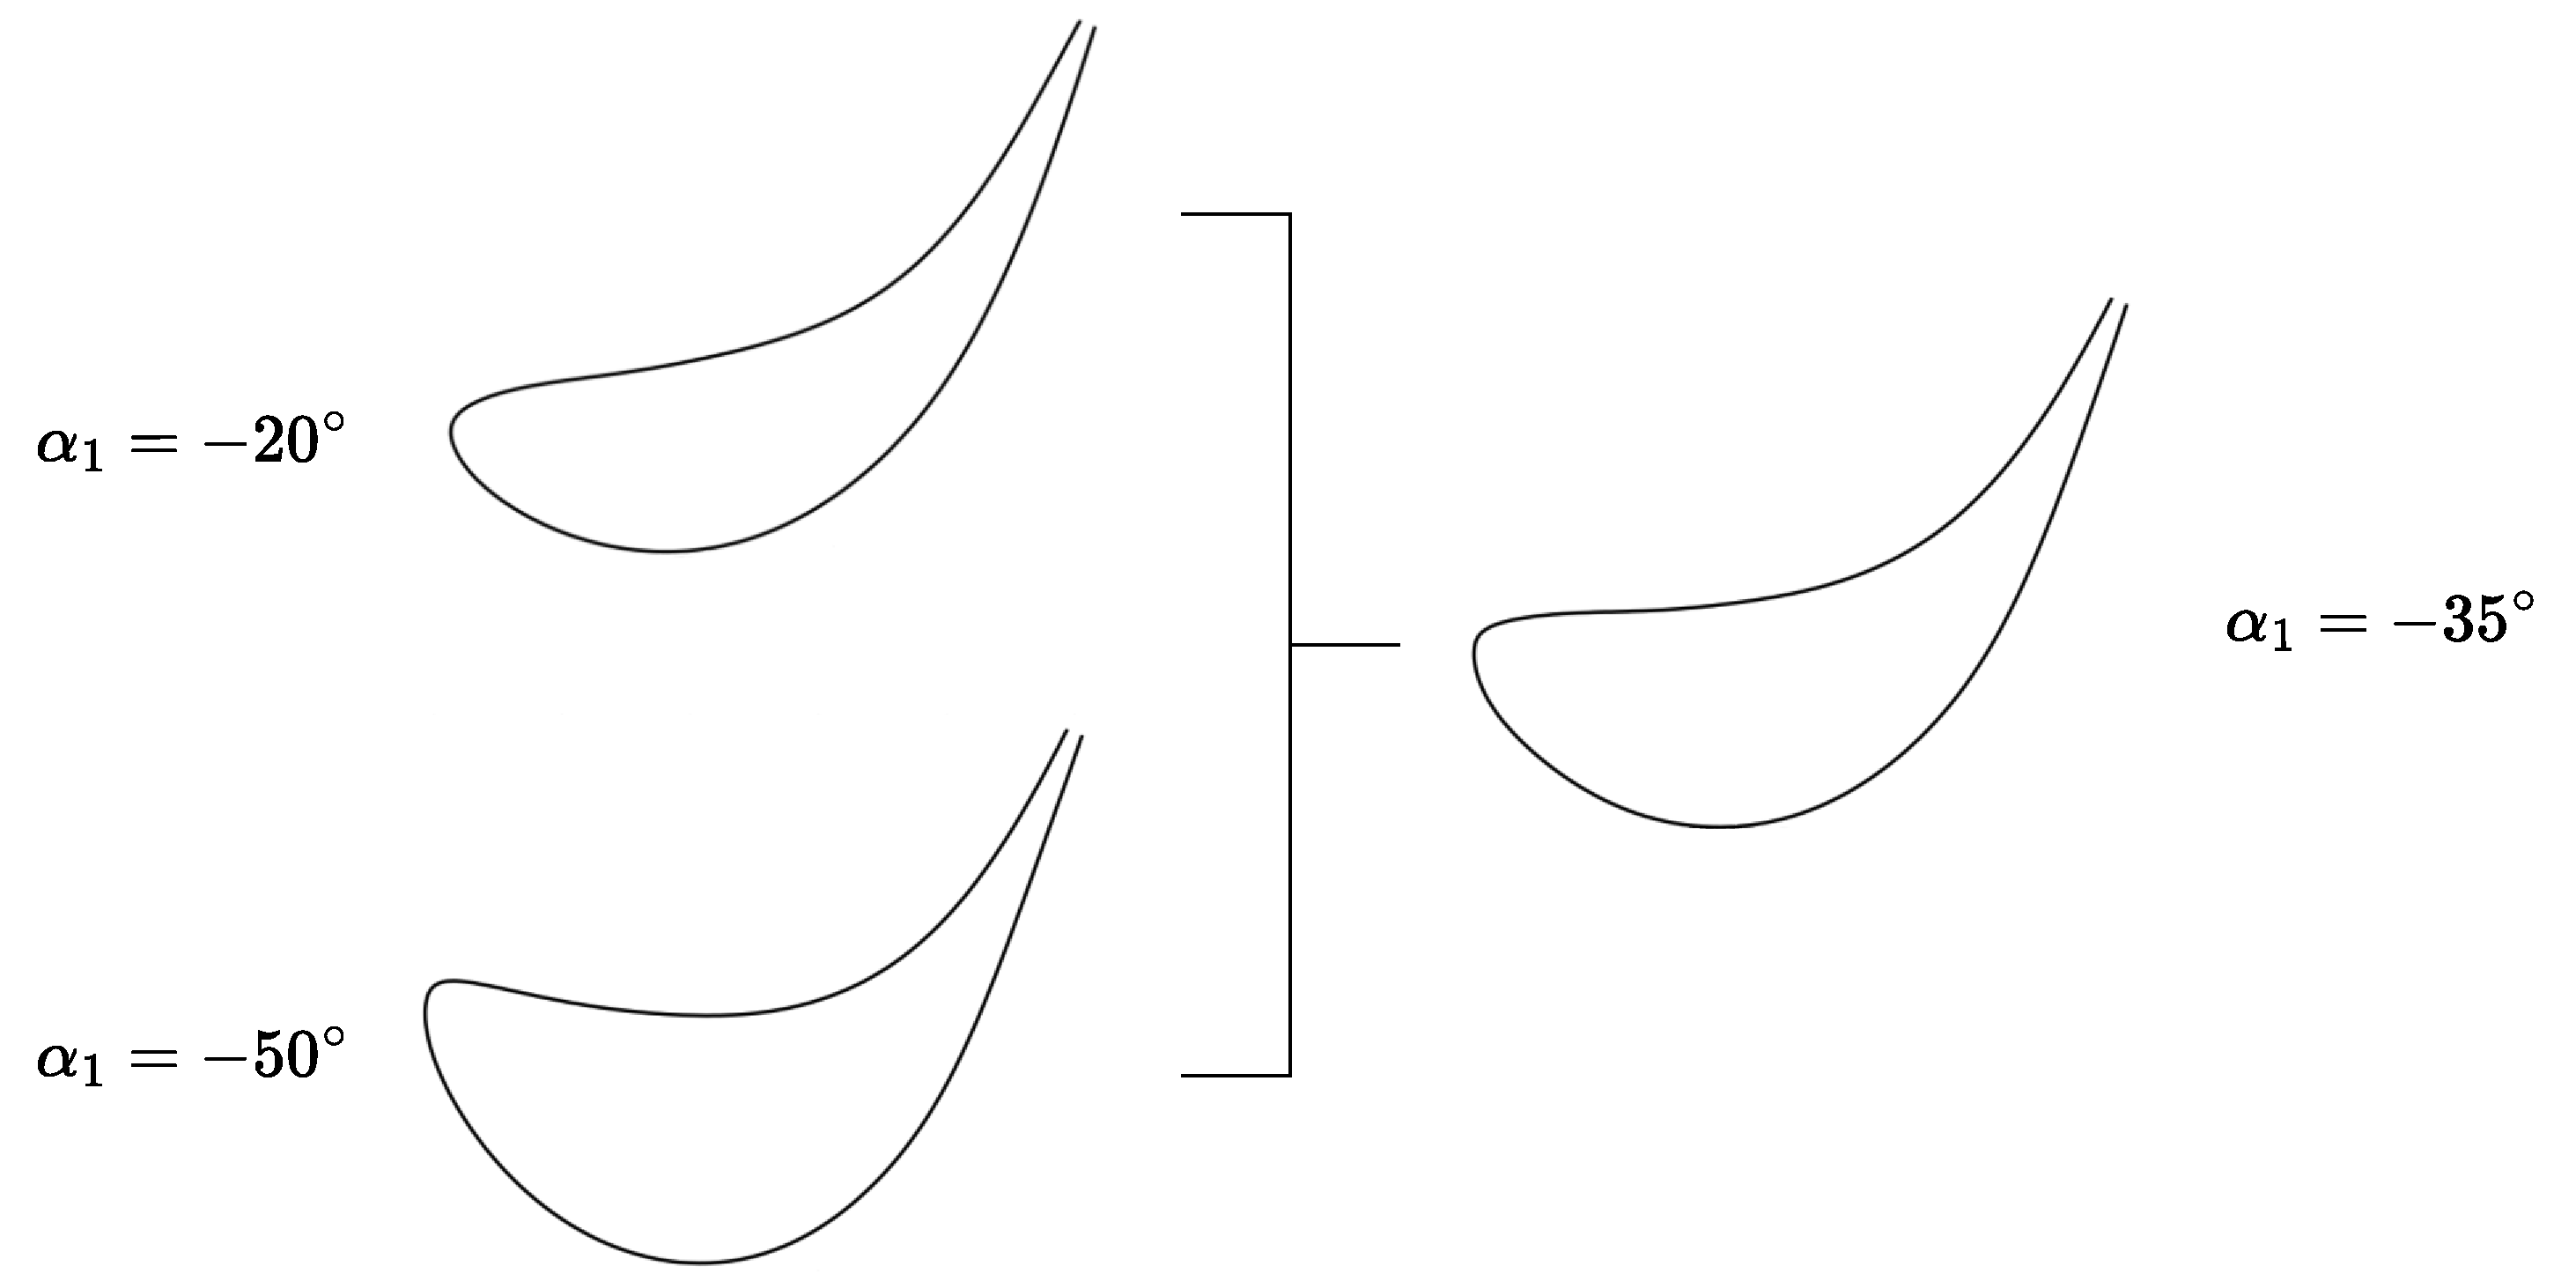
\includegraphics[page=1, scale=0.2]{./pdf/innerGeometry.pdf}
    \end{figure}
    From this guess, a \textbf{new optimization} of the inner point is made.
\end{frame}

\begin{frame}{Objectives \& constraints}
    \begin{columns}
        \column{0.5\textwidth}
            \begin{center}
                \renewcommand{\arraystretch}{2}
                \begin{tabularx}{1\textwidth} { 
                    || >{\centering\arraybackslash}X 
                    | >{\centering\arraybackslash}X 
                    | >{\centering\arraybackslash}X 
                    | >{\centering\arraybackslash}X || } 
                    \hline
                    Obj. & Min & Max & Points\\ [0.5ex] 
                    \hline\hline
                    $\frac{M_P}{M_{TE}}$ & $1.2$ & $1.4$ & 3 \\ [0.5ex]
                    \hline
                    $\frac{L_P}{L_{surf}}$ & $0.5$ & $0.6$ & 3 \\ [0.5ex]
                    \hline
                    $\frac{M_{LE}}{M_{TE}}\frac{M_2}{M_1}$ & $1.2$ & $1.8$ & 3 \\ [0.5ex]
                    \hline
                    $\frac{M_{PS}}{M_{TE}}\frac{M_2}{M_{1, ax}}$ & $0.8$ & $1.2$ & 3 \\ 
                    \hline
                \end{tabularx}
            \end{center}
        \column{0.5\textwidth}
            \begin{center}
                \renewcommand{\arraystretch}{2}
                \begin{tabularx}{1\textwidth} { 
                    || >{\centering\arraybackslash}X 
                    | >{\centering\arraybackslash}X 
                    | >{\centering\arraybackslash}X 
                    | >{\centering\arraybackslash}X || } 
                    \hline
                    Constr. & Min & Max & Points\\ [0.5ex] 
                    \hline\hline
                    $\alpha_1$ & $-50^{\circ}$ & $-20^{\circ}$ & 3 \\ [0.5ex]
                    \hline
                    $\alpha_2$ & $65^{\circ}$ & $72.5^{\circ}$ & 4 \\ [0.5ex]
                    \hline
                    $M_2$ & $0.4$ & $0.7$ & 3 \\ [0.5ex]
                    \hline
                    $Re$ & $6 \cdot 10^5$ & $6 \cdot 10^5$ & 1 \\ 
                    \hline
                \end{tabularx}
            \end{center}
    \end{columns}
\end{frame}
% \newcommand\WIDTH{3cm}
\newcommand\HEIGHT{1.25cm}
\newcommand\Ydist{0.2cm}
\newcommand\XPOS{1cm}
\newcommand\TOTheight{6.2cm}
\newcommand\TOTwidth{4cm}
\newcommand\PTS{1.2pt}
\newcommand\SHADOWred{50}
\newcommand\SHADOWgreen{30}
\newcommand\SHADOWblue{20}

\newcommand\blockHeight{1.5cm}
\newcommand\blockWidth{4cm}

\centering

\begin{tikzpicture}
    
    \node[draw,
        rectangle,
        % rounded corners,
        line width = \PTS,
        minimum height = \blockHeight,
        minimum width = \blockWidth,
        fill = blue!\SHADOWblue,
    ] (AI) at (0, 0) {\textbf{ML training}};

    \node[draw,
        rectangle,
        % rounded corners,
        line width = \PTS,
        minimum height = \blockHeight,
        minimum width = \blockHeight,
        fill = red!\SHADOWred,
    ] (X) at (-2, 3) {$\mathcal{X}$};

    \node[draw,
        rectangle,
        % rounded corners,
        line width = \PTS,
        minimum height = \blockHeight,
        minimum width = \blockHeight,
        fill = red!\SHADOWred,
    ] (Y) at (2, 3) {$\mathcal{Y}$};

    \node[draw,
        rectangle,
        % rounded corners,
        line width = \PTS,
        minimum height = \blockHeight,
        minimum width = \blockWidth,
        fill = green!\SHADOWgreen,
    ] (func) at (0, -3) {\textbf{ML function}};
    
    \node[draw,
        rectangle,
        % rounded corners,
        line width = \PTS,
        minimum height = \blockHeight,
        minimum width = \blockWidth
    ] (inputDuty) at (-6, -2) {\textbf{Aerodynamic Duty}};

    \node[draw,
        rectangle,
        % rounded corners,
        line width = \PTS,
        minimum height = \blockHeight,
        minimum width = \blockWidth
    ] (inputStyle) at (-6, -4) {\textbf{Aerodynamic Style}};

    \node[draw,
        rectangle,
        % rounded corners,
        line width = \PTS,
        minimum height = \blockHeight,
        minimum width = \blockWidth
    ] (outputGeometry) at (6, -4) {\textbf{Geometry}};

    \node[draw,
        rectangle,
        % rounded corners,
        line width = \PTS,
        minimum height = \blockHeight,
        minimum width = \blockWidth
    ] (outputProperty) at (6, -2) {\textbf{Losses}};

    \coordinate[] (c1) at (-2, 1.5) {};
    \coordinate[] (c2) at (2,  1.5) {};
    \coordinate[] (c3) at (0,  1.5) {};
    \coordinate[] (c4) at (-3,  -2) {};
    \coordinate[] (c5) at (-3,  -4) {};
    \coordinate[] (c6) at (-3,  -3) {};
    \coordinate[] (c7) at (3,  -2) {};
    \coordinate[] (c8) at (3,  -4) {};
    \coordinate[] (c9) at (3,  -3) {};

    \draw[-latex, line width=\PTS] (X.south) -- (c1) -- (c3) to (AI.north);
    \draw[-latex, line width=\PTS] (Y.south) -- (c2) -- (c3) to (AI.north);
    \draw[-latex, line width=\PTS] (AI) -- node[anchor=east] {\textit{test check}} (func);
    \draw[-latex, line width=\PTS] (inputDuty.east)  -- (c4) -- (c6) to (func.west);
    \draw[-latex, line width=\PTS] (inputStyle.east) -- (c5) -- (c6) to (func.west);
    \draw[-latex, line width=\PTS] (func.east) -- (c9) -- (c7) to (outputProperty.west);
    \draw[-latex, line width=\PTS] (func.east) -- (c9) -- (c8) to (outputGeometry.west);

\end{tikzpicture}

% \chapter{Modal Reduction}

\renewcommand\scaleBlade{0.64}

The following sections aim to explain the dimensionality reduction of the problem comparing the \textbf{Kulfan} based representation of the domain 
to a more \textbf{physical} representation using a \textbf{modal decomposition} of data. 

\section{Problem Framing}

The principal component analysis is one of the main methods for the dimensionality reduction of a problem~\cite{geron2022hands}. 
Unlike the machine learning part, the study is conducted only over the $\mathcal{Y}$ dataset. 

\section{Principal Component Analysis}

The method starts with a global analysis of the correlation between the different blade parameters:

\begin{itemize}
    \item $\gamma$, $\chi_1$ and $\chi_2$ for the camberline
    \item $A_{suct}$ for the suction side parametrization
    \item $A_{press}$ for the pressure side parametrization
    \item $pitch$
\end{itemize}

From this correlation analysis, the method extracts the main correlation directions. 
These directions will then define a vector which can be seen as one of the eigenvectors which defines the $\mathcal{Y}$ dataset.
After having computed the first direction, it is possible to compute the other \textit{modal directions}.

Listing~\ref{listing:PCA} shows the code used for the the principal component analysis of the $\mathcal{Y}$ dataset.

\lstinputlisting[style=customPy, caption=PCA decomposition, label=listing:PCA]{./code/PCA.txt}

Once computed all the \textit{modal directions}, it is possible to understand their importance for the 
definition of the whole dataset. For each \textit{modal direction} a variance index can be extracted.
This index represents the importance of the mode in the whole database. 
The higher the variance the higher the dataset coverage of its respective \textit{mode}.

A good dataset coverage is presented for a variance coverage above of $95\%$. 

Figure~\ref{fig:PCA} shows the variance distribution related to the dataset modes. 
With \textit{just} three modes it is possible to cover more than $95\%$ of the entire database.

\begin{figure}[H]
    \centering
    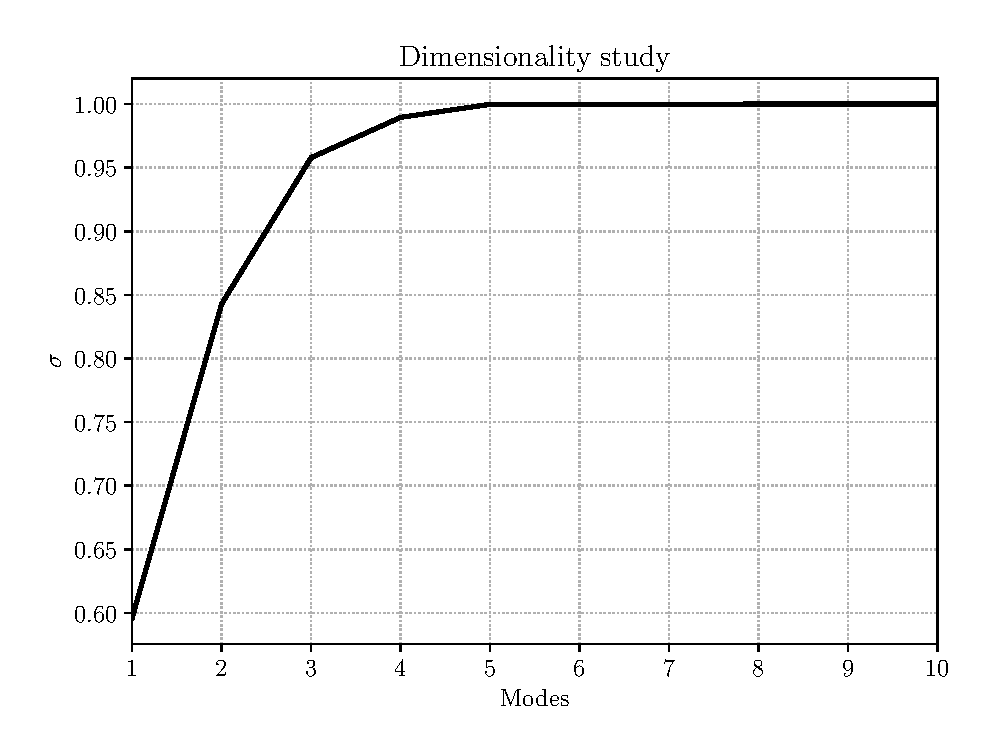
\includegraphics[scale=0.7]{./images/PCAmodes.eps}
    \caption{Principal Components of $\mathcal{Y}$ dataset.}
    \label{fig:PCA}
\end{figure}

\subsection{Modal Analysis}

% Having studied the main modes of $\mathcal{Y}$, it is possible to relate the load 
% variation due to these modes. This step allows to filter, again, the domain of study 
% passing through \textit{just} one dataset, $\mathcal{Y}$. This filtering action 
% does not have a direct corrleation to the $\mathcal{X}$ dataset but it can be seen better
% as the direct output of the main geometrical features of the $\mathcal{Y}$ dataset.

After analyzing the primary modes within $\mathcal{Y}$, it becomes feasible to establish a connection between the load variations attributed to these modes. This procedure facilitates a further refinement of the study domain by solely considering a single dataset, namely $\mathcal{Y}$. This filtering process is not directly linked to the $\mathcal{X}$ dataset; instead, it can be better understood as a direct manifestation of the key geometric characteristics inherent in the $\mathcal{Y}$ dataset.

Figure~\ref{fig:PCAmode1} shows the first mode. This mode is represented 
letting varying its amplitude over a reference blade. Figure~\ref{fig:PCAmode1}
represents also the load distribution varying the mode amplitude. From the plot 
it is possible understand that the first mode comprehends a lot of variation of the camberline.
This variation will result in a change of the suction side load, especially on the peak 
Mach number and on the leading edge loading.

\begin{figure}[H]
    \centering
    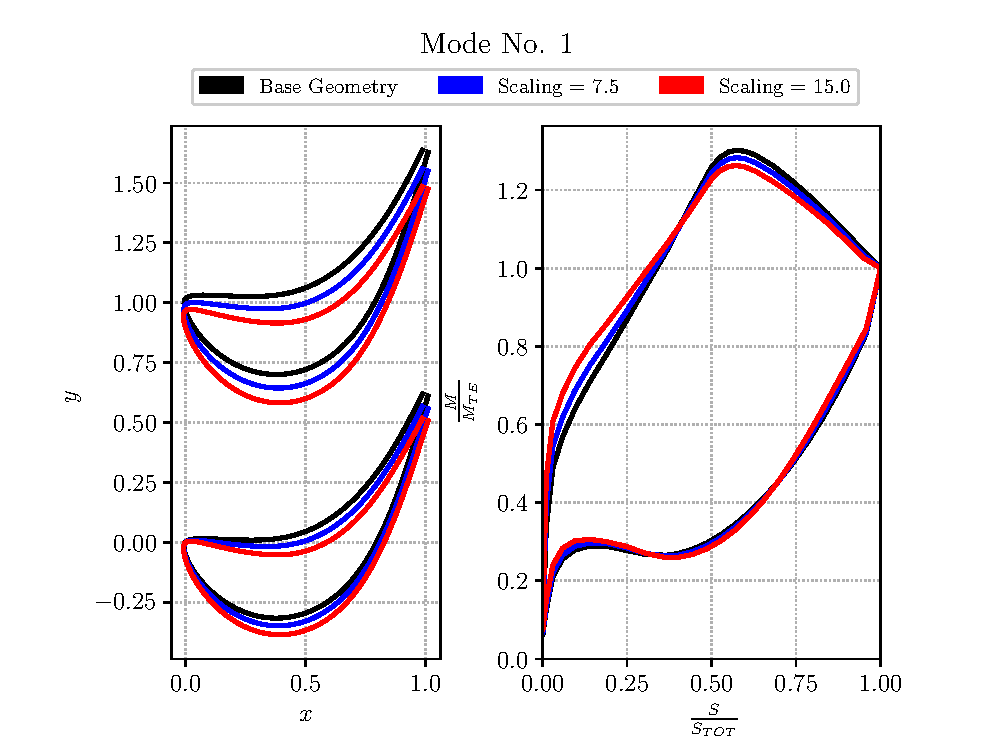
\includegraphics[scale=\scaleBlade]{./images/mode01.eps}
    \caption{Mode No. 1 with the respective modal loading distribution.}
    \label{fig:PCAmode1}
\end{figure}

\begin{figure}[H]
    \centering
    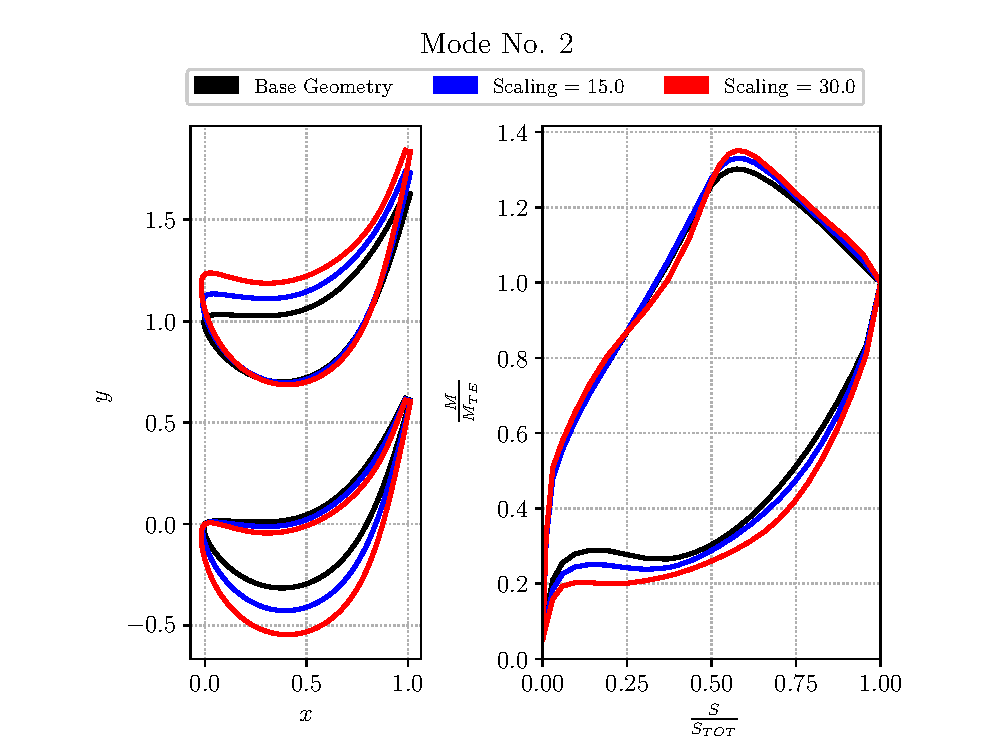
\includegraphics[scale=\scaleBlade]{./images/mode02.eps}
    \caption{Mode No. 2 with the respective modal loading distribution.}
    \label{fig:PCAmode2}
\end{figure}

The second mode, represented in Figure~\ref{fig:PCAmode2}, involves heavily the blade thickness variation.
The blade thickness variations do not change the loading at the leading edge on the suction side 
but it has an evident effect on the loading distribution at the leading edge on the pressure side. 
Even though the suction side leading edge is not affected by this mode, the peak Mach number 
on the suction side of the blade shows dependence on this mode; it can be seen as a mode 
which changes locally the load distribution over the suction side.

The first and second mode do not affect the position of the peak Mach number over the suction side.
The third mode, represented in Figure~\ref{fig:PCAmode3}, features the change in the position of the peak Mach number on the suction side. 
At the same time, appreciable changes are made on the pressure side Mach distribution.

\begin{figure}[H]
    \centering
    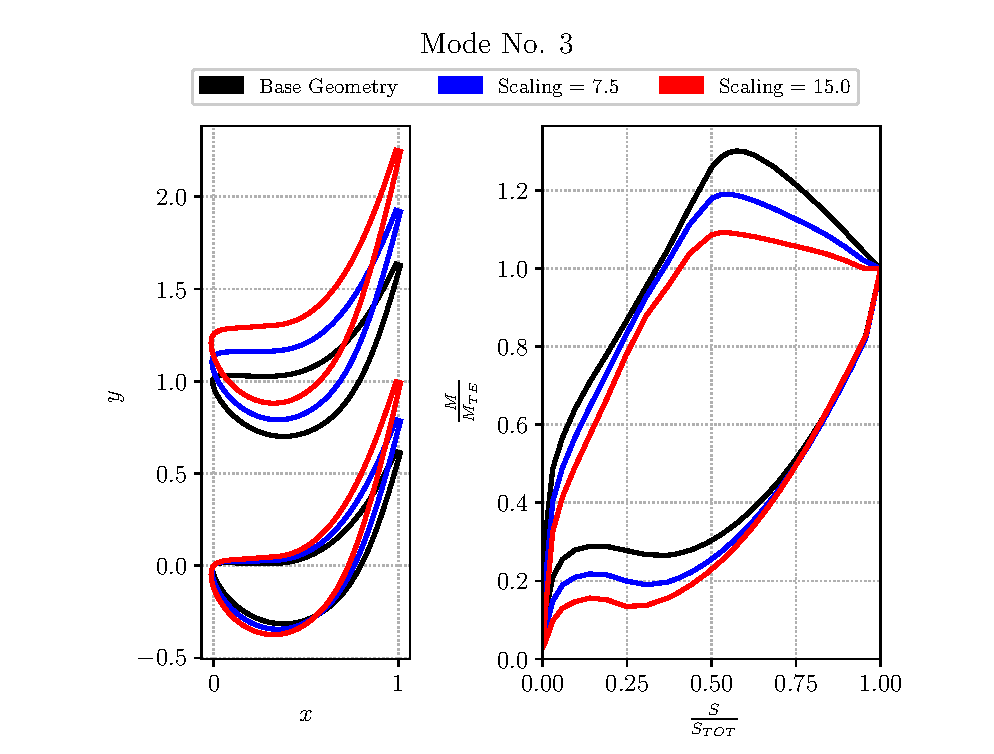
\includegraphics[scale=\scaleBlade]{./images/mode03.eps}
    \caption{Mode No. 3 with the respective modal loading distribution.}
    \label{fig:PCAmode3}
\end{figure} 

\begin{figure}[H]
    \centering
    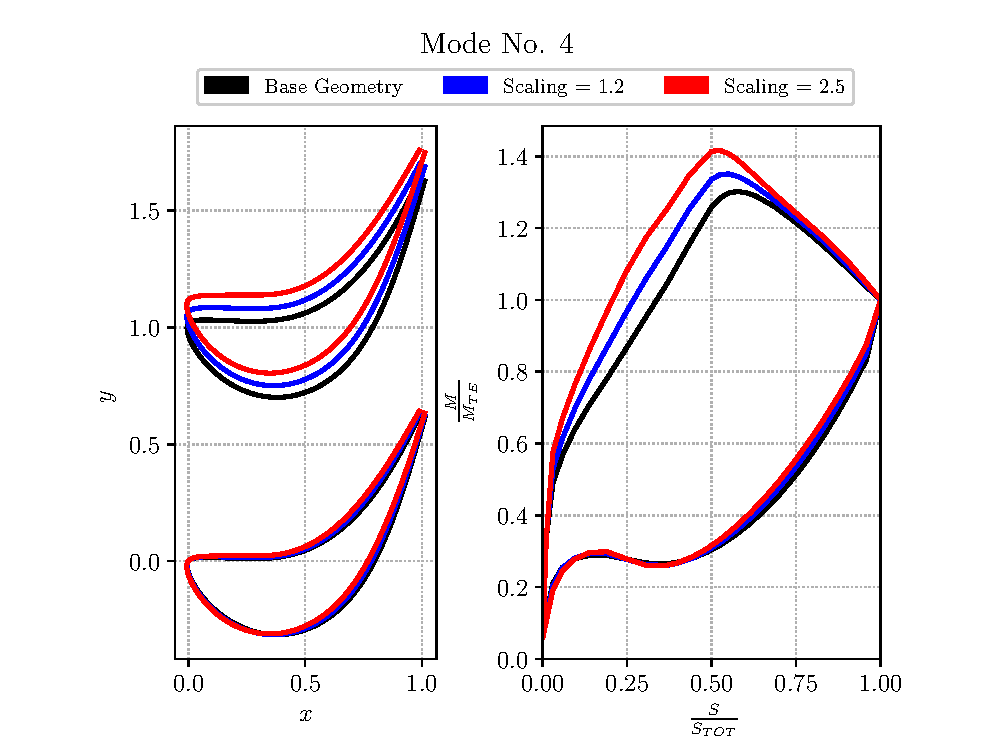
\includegraphics[scale=\scaleBlade]{./images/mode04.eps}
    \caption{Mode No. 4 with the respective modal loading distribution.}
    \label{fig:PCAmode4}
\end{figure}

Figure~\ref{fig:PCAmode4} represents the fourth dataset mode. Even though this mode can be seen as important, 
the dataset it spans is relatively small. This because the variance, $\sigma$, attributed to the fourth mode is smaller than the variance of its previous modal forms.
This mode features best the changes over the suction side of the blade. It is clear that the leading edge loading and the peak load on the suction side of the blade 
are heavily dependent on this mode. Even though this behavior, the influence of this mode on the dataset is of lower importance compared to the first mode.

\begin{figure}[H]
    \centering
    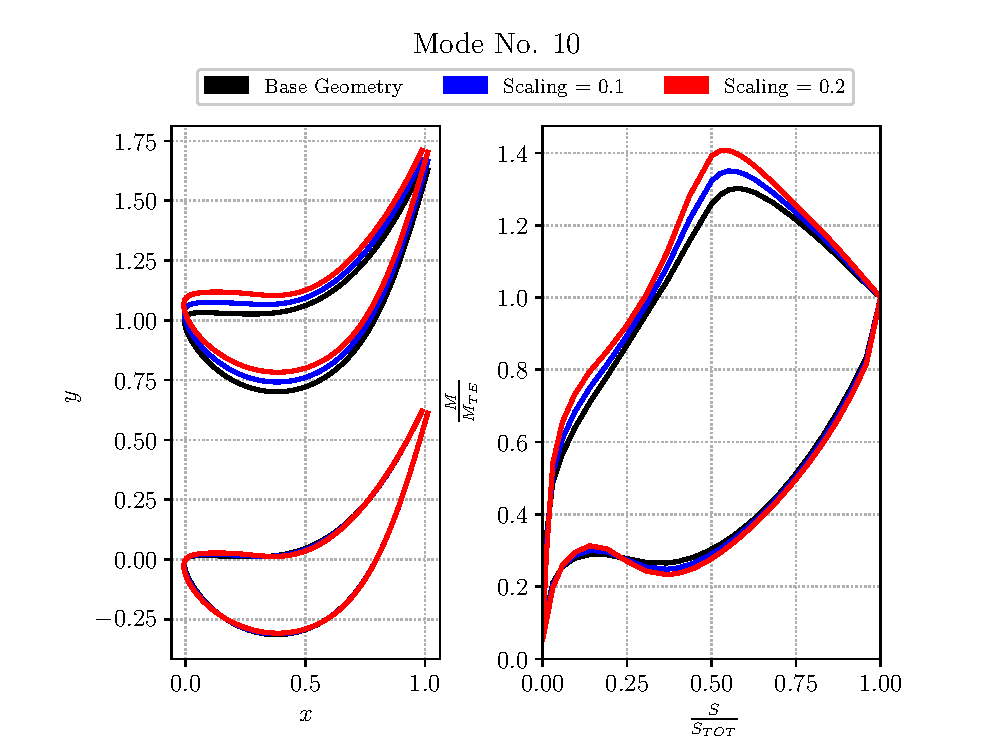
\includegraphics[scale=\scaleBlade]{./images/mode10.eps}
    \caption{Mode No. 10 with the respective modal loading distribution.}
    \label{fig:PCAmode10}
\end{figure}

The present work has shown the principal dataset modes - from the first mode to the third - but it
does not show the whole modal spectrum of the $\mathcal{Y}$ dataset. The following modes 
are more related to important modal forms from which important results can be taken. 

One of the most particular modal shapes are the 10th mode, the 30th mode and 42nd mode, the last mode.
These modes underline important physical properties:

\begin{itemize}
    \item the fact that the modal spectrum does not follow the same engineering strategy for the design of a section 
    but it relies \textbf{only} on the dataset: mode 10th.
    \item there are modes which act on a very specific part of the loading distribution: mode 30th.
    \item there are modes which can be seen as noise and have low importance in the section design process: mode 42nd.
\end{itemize}

Figure~\ref{fig:PCAmode10} shows the 10th mode. This mode affects mainly the pitch degree of freedom.
This mode changes the load distribution over the blade because a variation of the channel size. 
At the same time, the exit flow angle is heavily dependent on the solidity ($solidity = \frac{pitch}{chord}$) which is related to the pitch.

\begin{figure}[H]
    \centering
    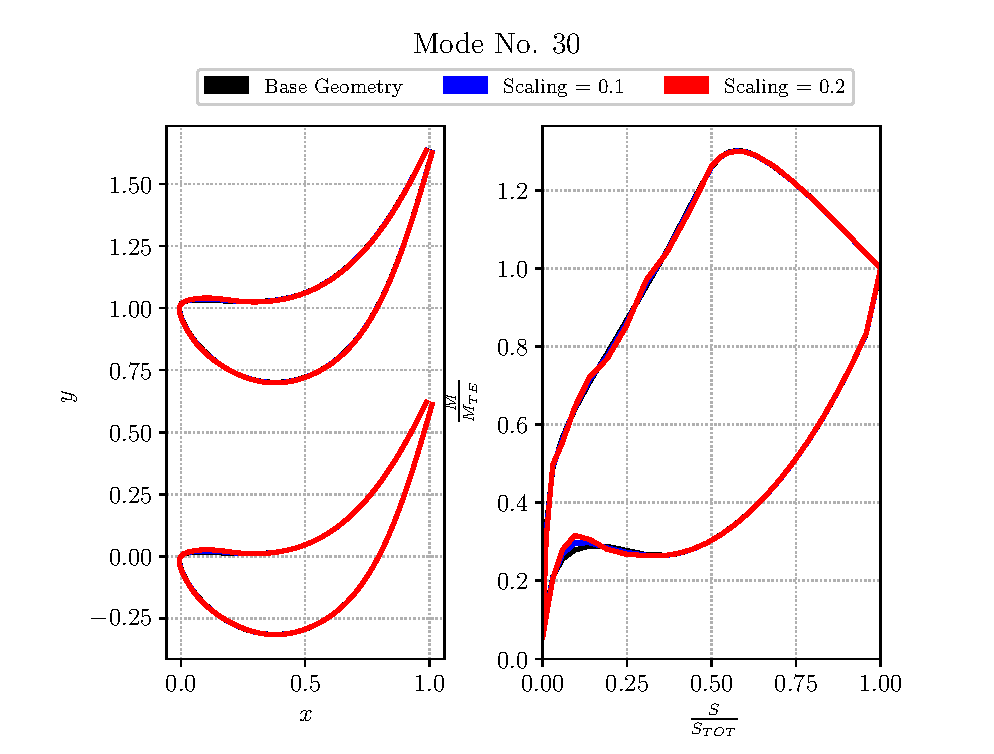
\includegraphics[scale=\scaleBlade]{./images/mode30.eps}
    \caption{Mode No. 30 with the respective modal loading distribution.}
    \label{fig:PCAmode30}
\end{figure}

Even though the 10th mode can be seen as an important mode because of the turbomachinery theory, 
it is of secondary importance inside the modal behavior of the system. This because the previous modes
\textbf{span much more space} than the 10th.

Using Figure~\ref{fig:PCAmode30}, it is possible to understand the influence, both 
over geometry and loading, of a low-variance mode. In this figure, the main geometrical 
variation is made over the pressure side at the leading edge of the blade. This change 
affects mostly the local Mach fraction distribution at the leading edge on the pressure side.
With this mode, it is possible to highlight the fact that avoiding modes with low variance 
does not generate huge errors in the geometry representation.

Figure~\ref{fig:PCAmode42} shows the last modal shape. This shape can be seen as 
a wobbling noise around the blade and it has the lowest importance in the 
representation of the blade domain. As the 30th modal shape, the 42nd mode 
can be dropped off for a modal representation of a blade without loosing accuracy
both in geometry and loading.

\begin{figure}[H]
    \centering
    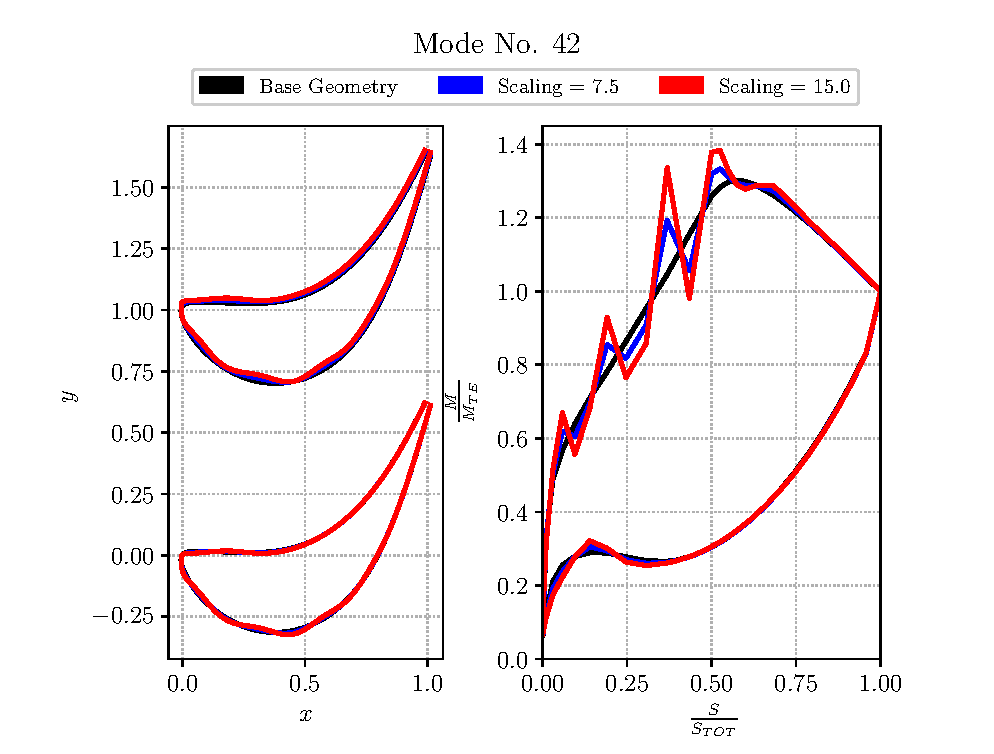
\includegraphics[scale=\scaleBlade]{./images/mode42.eps}
    \caption{Mode No. 42 with the respective modal loading distribution.}
    \label{fig:PCAmode42}
\end{figure}

% \chapter{Conclusions}

This chapter concludes the present work and highlights the main \textbf{results}, \textbf{limitations}, and possible \textbf{achievable improvements}.

\section{Introduction and Reiteration}

In this study, a groundbreaking design methodology has been developed for the field of turbomachinery blade design. This novel approach eliminates the need for conventional CFD simulations, significantly reducing design time while establishing insightful correlations between data and blade geometries.

\section{Summary of Findings}

The most crucial outcome of this research is the successful validation of the proposed methodology. It demonstrates applicability in blade design, offering speed and the ability to break down the design space into principal geometrical modes.

\section{Implication and Significance}

These identified modes present the opportunity to design blades more efficiently, employing a limited number of parameters compared to traditional blade parametrization methods. The establishment of a correlation between blade geometry and parametrized loading distribution further empowers the model. Simultaneously, the model defines the design's limitations in terms of loading, granting designers a comprehensive understanding of the design space and constraints in turbomachinery design.

\section{Limitations}

It's important to acknowledge that the model's boundaries are defined by the laws of physics. The sensitivity of database generation to loading parametrization highlights the close connection to physics. Moreover, the quality of the input database significantly impacts the quality of the resulting blades. Ensuring a high-quality database is essential for optimal results.

\section{Future Directions}

Future research directions could explore how blade geometry behaves with variations in the Reynolds number. Investigating blade geometry changes under diverse loading conditions also holds promise for advancing the methodology.

% \section{Final Reflections}

% The model's practicality in the industry is evident, serving as an initial design layer for blade generation. It offers a comprehensive range of macroscopic values that hold pivotal importance in the realm of turbomachinery.

\section{Closing Statements}

% The impact of this innovative methodology cannot be overstated. 
The model's practicality in the industry is evident, serving as an initial design layer for blade generation. By seamlessly integrating physics and machine learning through data, it opens up a new avenue for designing turbomachinery systems. This efficient tool accelerates the design process, making it accessible to designers across the field. The profound significance lies in its ability to reshape the design landscape, creating a faster and more intuitive approach for designing turbomachinery systems.

% %-------------------------------------------------------------------------
% %	BIBLIOGRAPHY
% %-------------------------------------------------------------------------

% \addtocontents{toc}{\vspace{2em}} % Add a gap in the Contents, for aesthetics
% \bibliography{biblio} % The references information are stored in the file named "Thesis_bibliography.bib"

% %-------------------------------------------------------------------------
% %	APPENDICES
% %-------------------------------------------------------------------------

% \cleardoublepage
% \addtocontents{toc}{\vspace{2em}} % Add a gap in the Contents, for aesthetics
% \appendix
% \chapter{Appendix A}
% If you need to include an appendix to support the research in your thesis, you can place it at the end of the manuscript.
% An appendix contains supplementary material (figures, tables, data, codes, mathematical proofs, surveys, \dots)
% which supplement the main results contained in the previous chapters.

% \chapter{Appendix B}
% It may be necessary to include another appendix to better organize the presentation of supplementary material.

% ACKNOWLEDGEMENTS
% \cleardoublepage
% \thispagestyle{empty}
% \epigraph{\textbf{Discipline, doing what you hate to do but do it like you love it.}}{\textit{Mike Tyson}}
% \cleardoublepage

\end{document}
